\documentclass[a4paper, 14pt, oneside]{extbook}
\usepackage[italian]{babel} %Capitoli in italiano
\usepackage[T1]{fontenc}
\usepackage[utf8x]{inputenc}
\usepackage{geometry}
\usepackage{courier}
\usepackage[bookmarks]{hyperref}
\newgeometry{
left=   1.5 in,
bottom= 1.5 in,
right=  1 in,
top=    1 in
}
\usepackage{booktabs}
\usepackage{longtable}
\usepackage{array}
\usepackage{ragged2e}
\usepackage{needspace}
\usepackage{fancyhdr}

% Grafica
\usepackage{graphicx,pstricks}
\usepackage{graphics}
\graphicspath{{img/}}

% Package usati per il frontespizio
\usepackage[T1]{fontenc}
\usepackage{lmodern}

\usepackage{xcolor}
\usepackage{tikz}
\usetikzlibrary{patterns}

\usepackage{pgf-pie}
\usepackage{pgfplots}
\pgfplotsset{width=7cm,compat=1.8}

\usepackage{listings}
\usepackage{tcolorbox}
\tcbuselibrary{listings,skins,breakable}

\usepackage{enumitem}


%Aggiunte
\usepackage{float}

%Algorithm
\usepackage{algorithm}
\usepackage[noend]{algpseudocode}

\setlength\headheight{44.2pt}

%Page Style
\usepackage{setspace}

%\setstretch{2.5} 
\doublespace

%\cfoot{\thepage}
\lhead[]{}
\rhead[]{\leftmark}

\pagestyle{fancy}{
\lhead{
\includegraphics[scale=0.3]{img/logo/hlogo.png}}
\rhead{\footnotesize{Titolo abbreviato come intestazione}}
}

%Other
\usepackage{comment}
\usepackage{amsmath}

%Testo riempitivo
\usepackage{lipsum}

\setlength{\parindent}{0pt} % Toglie il rientro all'inizio dei paragrafi

\usepackage{booktabs}
\usepackage{graphicx}
\usepackage{xurl} % permette di andare a capo ovunque nell'URL
\usepackage{mdframed}
\usepackage{multirow}
\usepackage{tabularx}
\usepackage{array}
\usepackage{fvextra}
\usepackage{tocloft}
\usepackage{comment}

% Titoli delle liste
\renewcommand{\listfigurename}{Lista delle figure}
\renewcommand{\listtablename}{Lista delle tabelle}

% Prefisso prima del numero
\renewcommand{\cftfigpresnum}{Figura~}
\renewcommand{\cfttabpresnum}{Tabella~}

% Spazio dopo il numero
\renewcommand{\cftfigaftersnum}{\quad}
\renewcommand{\cfttabaftersnum}{\quad}

% Larghezza riservata a "Figura 4.1" / "Tabella 5.3"
\setlength{\cftfignumwidth}{5.5em}
\setlength{\cfttabnumwidth}{6.5em}

% Spazio verticale tra le voci
\setlength{\cftbeforefigskip}{8pt}
\setlength{\cftbeforetabskip}{8pt}

\newboolean{showcomments}
\setboolean{showcomments}{true}
\ifthenelse{\boolean{showcomments}}
{\newcommand{\nb}[2]{
		\fcolorbox{black}{yellow}{\bfseries\sffamily\scriptsize#1}
		{\sf\small$\blacktriangleright$\textit{#2}$\blacktriangleleft$}
	}
	\newcommand{\version}{\emph{\scriptsize$-$working$-$}}
    \newcommand{\ugh}[1]{\textcolor{red}{\uwave{#1}}} % please rephrase
   % \newcommand{\ins}[1]{\textcolor{blue}{#1}} % please insert
   \newcommand{\ins}[1]{\textcolor{blue}{#1}} % please insert
   \newcommand{\del}[1]{\textcolor{red}{\st{#1}}} % please delete
   \newcommand{\chg}[2]{\textcolor{red}{\st{#1}}{$\rightarrow$}\textcolor{blue}{\uline{#2}}} % please change
   %\newcommand{\inspar}[1]{\color{blue}{#1}\color{blue}}
   \newcommand{\delpar}[1]{\textcolor{red}{#1}}
   \newcommand{\inspar}[1]{\textcolor{blue}{#1}}
   \newcommand{\insR}[1]{\textcolor{blue}{#1}} % please insert
   \newcommand{\delR}[1]{\textcolor{red}{\st{#1}}} % please delete
}
{\newcommand{\nb}[2]{}
	\newcommand{\version}{}
}

\newcommand\marco[1]{\nb{Marco}{\color{teal}#1}}
\newcommand\domenico[1]{\nb{Mimmo}{\color{blue}#1}}
\newcommand\annarita[1]{\nb{Anna Rita}{\color{magenta}#1}}
\newcommand\tiziano[1]{\nb{Domenico}{\color{green}#1}}
\newcommand\patrizio[1]{\nb{Pasquale}{\color{red}#1}}



\begin{document}

%\maketitle
\begin{titlepage}
\thispagestyle{empty}
\raggedright % Allinea a sinistra

\begin{tikzpicture}
\node[anchor=south west] at (4,0) {
\includegraphics[scale=0.75]{img/logo/logo_copertina_1}};
\node[anchor=south west] at (0,1.5) {
\includegraphics{img/logo/logo_copertina_2}};
\node[anchor=south west] at (0,0.5) {\textsf{Scuola Politecnica e delle Scienze di Base}};
\node[anchor=south west] at (0,0) {\textsf{Corso di Laurea Magistrale in Ingegneria Informatica}};
\end{tikzpicture}

\vfill

{\large Tesi di Laurea Magistrale in Ingegneria Informatica}
\\[1cm]
%Alternativa 1: Rilevazione di anti-pattern architetturali in sistemi a microservizi: un approccio basato su LLM e confronto con strumenti di analisi statica
{\textbf{\textit{\LARGE Rilevazione di anti-pattern in architetture a microservizi tramite LLM: confronto con tecniche di analisi statica}}}
\\[1cm]
{\large Anno Accademico 2025/2026}

\vfill


\begin{table}[h]
Relatore
\\
\textbf{Ch.ma Prof.ssa Anna Rita Fasolino}
\\
Correlatore
\\
\textbf{Ing. Marco De Luca}
\\ \\
{\raggedright Candidato}
\\
\textbf{Antimo Barbato}
\\
\textbf{matr. M63001079}
\end{table}

\end{titlepage}
\frontmatter

\thispagestyle{empty}

\vspace*{0.28\textheight}

\begin{flushright}
\begin{minipage}{0.62\textwidth}
\itshape
``La nostra gloria più grande non sta nel non cadere mai,
ma nel risollevarci ogni volta che cadiamo.''\\[1em]
\normalfont\raggedleft
--- Confucio
\end{minipage}
\end{flushright}

\vfill

\chapter{Abstract} 

Le architetture a microservizi offrono modularità, scalabilità e indipendenza di deployment, ma introducono anche una maggiore complessità architetturale e il rischio di anti-pattern difficili da individuare con tecniche tradizionali. In questo contesto, la tesi analizza il potenziale dei Large Language Models (LLM) per la detection di anti-pattern in sistemi a microservizi, valutandone sia l’efficacia autonoma sia il confronto con MARS, uno strumento state-of-the-art basato su analisi statica rule-based e metamodello.

L’esperimento è stato condotto su 13 repository open-source, considerando 16 anti-pattern e tre modelli linguistici di ultima generazione: ChatGPT, Gemini e Qwen. La procedura ha previsto 624 inferenze indipendenti, realizzate mediante una pipeline che combina aggregazione della codebase con Repomix, estrazione di metriche strutturali e prompt engineering controllato. Le prestazioni sono state valutate rispetto a una ground truth manuale, utilizzando Precision, Recall e F1-score.

I risultati mostrano che gli LLM ottengono buone prestazioni quando l’anti-pattern lascia tracce relativamente esplicite nella repository, come nel caso di \textit{Hardcoded Endpoint}, \textit{No API Versioning}, \textit{No CI/CD} e \textit{No API Gateway}. Le prestazioni peggiorano invece nei casi che richiedono una ricostruzione relazionale esplicita, una validazione architetturale più profonda o la combinazione di segnali quantitativi e qualitativi, come \textit{Cyclic Dependency}, \textit{Shared Libraries}, \textit{Mega-Service} e \textit{Nano-Service}. Il confronto con MARS evidenzia una forte complementarità tra i due approcci: gli LLM risultano più efficaci nei casi che richiedono flessibilità interpretativa e generalizzazione, mentre MARS prevale quando il difetto può essere ricondotto a regole deterministiche su dipendenze, configurazioni o soglie numeriche.

Nel complesso, la tesi mostra che gli LLM rappresentano uno strumento promettente per l’analisi architetturale dei microservizi, ma che la loro efficacia dipende in misura significativa dalla definizione operativa degli anti-pattern, dalla qualità del prompt e dalla costruzione del contesto di input. I risultati suggeriscono infine che la direzione più promettente sia un paradigma ibrido, capace di combinare la robustezza dell’analisi statica con la flessibilità interpretativa dei modelli linguistici.






%\chapter*{Lista delle figure}
\begin{enumerate}
    \item Microservice Antipatterns Research Software.
    \item Pipeline dell'esperimento.
\end{enumerate}
%\chapter*{Lista delle tabelle}
\begin{enumerate}
    \item File di configurazione utilizzati da MARS per la detection degli anti-pattern.
    \item Lista LLM utilizzati.
    \item Elenco delle repository a microservizi analizzate nell'esperimento, con le relative metriche dimensionali.
    \item Definizioni degli Anti-Pattern utilizzate nei Prompt.
    \item Risultati comparativi: ChatGPT, Qwen e Gemini con F1-Score.
    \item Confronto completo delle performance (Precision e Recall) sulle tre repository > 400k Token.
    \item Sintesi qualitativa dei risultati degli LLM per anti-pattern.
    \item Risultati comparativi: ChatGPT, Qwen, Gemini e MARS con F1-Score.
    \item Sintesi comparativa del confronto tra LLM e MARS per anti-pattern.
\end{enumerate}

{\setstretch{1.5}
\tableofcontents
}

\cleardoublepage
\listoffigures

\cleardoublepage
\listoftables

\cleardoublepage
\chapter*{Lista delle abbreviazioni}
\begin{description}
    \item[API] Application Programming Interface
    \item[AP] Anti-Pattern
    \item[BFF] Backend for Frontend
    \item[CD] Cyclic Dependency
    \item[CI/CD] Continuous Integration / Continuous Delivery
    \item[CoT] Chain-of-Thought
    \item[CQRS] Command Query Responsibility Segregation
    \item[CRUD] Create, Read, Update, Delete
    \item[DDD] Domain-Driven Design
    \item[DFD] Data Flow Diagram
    \item[DTO] Data Transfer Object
    \item[ESB] Enterprise Service Bus
    \item[FN] False Negative
    \item[FP] False Positive
    \item[F1] F1-score
    \item[GT] Ground Truth
    \item[HE] Hardcoded Endpoint
    \item[HTTP] Hypertext Transfer Protocol
    \item[IaC] Infrastructure-as-Code
    \item[IM] Insufficient Monitoring
    \item[IPC] Interprocess Communication
    \item[LL] Local Logging
    \item[LLM] Large Language Model
    \item[LOC] Lines of Code
    \item[MARS] Microservice Antipatterns Research Software
    \item[MC] Manual Configuration
    \item[MS] Mega-Service
    \item[MSA] Microservice Architecture
    \item[MSIPH] Multiple Service Instances Per Host
    \item[NAG] No API Gateway
    \item[NAV] No API Versioning
    \item[NCI] No CI/CD
    \item[NHC] No Health Check
    \item[NS] Nano-Service
    \item[POM] Project Object Model
    \item[RAG] Retrieval-Augmented Generation
    \item[REST] Representational State Transfer
    \item[RQ] Research Question
    \item[SL] Shared Libraries
    \item[SOA] Service-Oriented Architecture
    \item[SP] Shared Persistency
    \item[SQL] Structured Query Language
    \item[TLD] Top-Level Domain
    \item[TO] Timeouts
    \item[TP] True Positive
    \item[URI] Uniform Resource Identifier
    \item[URL] Uniform Resource Locator
    \item[WC] Wrong Cuts
    \item[WebUI] Web User Interface
\end{description}
\mainmatter

\chapter{Introduzione}

\section{Contesto e Motivazioni}

Le architetture a microservizi si sono progressivamente affermate come uno dei paradigmi più rilevanti per la realizzazione di sistemi software distribuiti, grazie alla loro capacità di favorire modularità, scalabilità, indipendenza di deployment e maggiore flessibilità evolutiva \cite{CernyCatalogo, Dragoni2017}. Tuttavia, tali vantaggi si accompagnano a un aumento della complessità architetturale, poiché il comportamento complessivo del sistema non dipende più soltanto dalla qualità dei singoli moduli, ma anche dalle modalità con cui i servizi vengono decomposti, configurati e fatti interagire tra loro \cite{CernyCatalogo, Dragoni2017, Soldani2018PainsGains}.

In questo contesto, gli anti-pattern architetturali assumono un ruolo particolarmente rilevante. Essi rappresentano soluzioni progettuali apparentemente accettabili, ma in grado di produrre nel tempo conseguenze negative sulla qualità del software, compromettendo manutenibilità, autonomia dei servizi, osservabilità e resilienza del sistema \cite{CernyCatalogo}. La loro individuazione tempestiva è quindi essenziale per supportare l’analisi architetturale e prevenire il consolidarsi di decisioni progettuali non ottimali.

La rilevanza del tema emerge anche sul piano industriale. Alcuni report di mercato mostrano infatti una crescita significativa dell’interesse verso l’architettura a microservizi, trainata dalla diffusione del cloud, delle pratiche DevOps, dell’orchestrazione di container e dello sviluppo di applicazioni distribuite basate su API \cite{dati_micro}. Sebbene tali dati abbiano natura principalmente descrittiva e vadano interpretati con cautela, essi confermano la centralità pratica del paradigma e la conseguente importanza di strumenti efficaci per la comprensione e la valutazione della qualità architetturale.

\section{Problemi di ricerca}

Nonostante la crescente diffusione delle architetture a microservizi, la detection automatica dei relativi anti-pattern rimane un problema aperto. Gli strumenti tradizionali di analisi statica risultano spesso efficaci nell’individuare anomalie locali o dipendenze specifiche, ma incontrano maggiori difficoltà quando il difetto emerge dall’interazione tra più servizi o richiede una lettura sistemica dell’intera codebase \cite{CernyCatalogo, MSAnose}. Strumenti più evoluti, come MARS, hanno certamente ampliato la copertura del problema attraverso l’uso di metamodelli e regole statiche, ma presentano ancora limiti legati alla dipendenza da euristiche, whitelist, blacklist e soglie predefinite \cite{MARS}.

Parallelamente, i Large Language Models hanno mostrato capacità promettenti in numerosi compiti di analisi del software, ma il loro impiego nella detection di anti-pattern architetturali in sistemi a microservizi è ancora poco esplorato. Gli studi esistenti si concentrano prevalentemente su code smells locali o su forme preliminari di analisi architetturale, come nel caso di approcci che utilizzano LLM per interpretare artefatti di Infrastructure-as-Code \cite{iac_llm}. Rimane quindi aperta la questione se tali modelli possano supportare efficacemente l’identificazione di difetti architetturali complessi, soprattutto nei casi in cui sia richiesta una lettura contestuale e inter-servizio della repository \cite{contextwindows_llm, prompteng}.

\section{Obiettivi della tesi}

Alla luce di queste considerazioni, la presente tesi si propone di valutare empiricamente l’impiego dei Large Language Models nella detection di anti-pattern in architetture a microservizi. L’obiettivo non è soltanto misurare le prestazioni dei modelli in termini quantitativi, ma anche comprendere in quali casi essi risultino più efficaci, quali limiti mostrino e in che misura possano costituire un’alternativa o un complemento rispetto agli strumenti di detection tradizionali.

Il lavoro di tesi, quindi, punta a:
\begin{itemize}
    \item valutare l’efficacia di diversi LLM nell’individuazione di un insieme eterogeneo di anti-pattern in repository reali a microservizi;
    \item confrontare i risultati ottenuti con quelli di MARS, uno degli strumenti per la detection di anti-pattern in questo dominio \cite{MARS};
    \item analizzare qualitativamente i casi in cui i modelli riescono o falliscono, evidenziando il ruolo della definizione operativa dell’anti-pattern, del prompt e della costruzione dell’input;
    \item discutere le implicazioni metodologiche emerse dall’esperimento, anche in vista di possibili approcci ibridi tra analisi statica e modelli linguistici.
\end{itemize}

Le prestazioni dei modelli sono state valutate mediante l'impiego di una \textit{ground truth} manuale resa disponibile dallo studio MARS \cite{MARS}.


\section{Research Questions}

Per raggiungere gli obiettivi citati precedentemente, la tesi si articola attorno alle seguenti domande di ricerca:

\begin{itemize}
    %\item \textbf{RQ1: How effective are LLMs at detecting anti-patterns in MSAs?}
    \item \textbf{RQ1: Quanto sono efficaci gli LLM nel rilevare gli anti-pattern nelle MSA?}
    
    Questa domanda mira a valutare l’efficacia dei Large Language Models nell’identificazione di anti-pattern architetturali in sistemi a microservizi, considerando sia i risultati quantitativi sia la variabilità delle prestazioni in funzione della natura del difetto analizzato.
    
    %\item \textbf{RQ2: How do LLMs compare against state-of-the-art static analysis tools for anti-pattern detection in MSAs?}

    \item \textbf{RQ2: Come si confrontano gli LLM con gli strumenti di analisi statica allo stato dell’arte per il rilevamento degli anti-pattern nelle MSA?}
    
    Questa domanda intende confrontare criticamente il comportamento degli LLM con quello di uno strumento \textit{rule-based} basato su metamodello, al fine di comprendere se i modelli linguistici possano eguagliare, superare oppure integrare gli approcci tradizionali di detection.
\end{itemize}

\section{Struttura della tesi}

La tesi è organizzata come segue.

Nel Capitolo 2 vengono introdotti i fondamenti teorici relativi alle architetture a microservizi e ai principali concetti utili per inquadrare il dominio applicativo. Nel Capitolo 3 viene presentato il tema degli anti-pattern nelle architetture a microservizi, con particolare attenzione al catalogo proposto in letteratura e alle categorie considerate nello studio. Nel Capitolo 4 vengono analizzati gli strumenti e gli approcci alla detection degli anti-pattern, approfondendo sia gli strumenti tradizionali, con particolare riferimento a MARS, sia il potenziale impiego dei Large Language Models e delle tecniche di \textit{prompt engineering}. Nel Capitolo 5 viene descritto nel dettaglio l’esperimento condotto, inclusi dataset, modelli, pipeline, costruzione dell’input e procedura di valutazione. Nel Capitolo 6 vengono presentati e discussi i risultati ottenuti, rispondendo alle Research Questions e analizzando anche le lezioni apprese e le principali minacce alla validità. Infine, il Capitolo 7 riassume le conclusioni del lavoro e propone alcune possibili direzioni di sviluppo futuro.




 \chapter{Background}

\section[Dalle applicazioni monolitiche alle prime forme di modularità]%
{Dalle applicazioni monolitiche \\ alle prime forme di modularità}
Le applicazioni monolitiche hanno rappresentato a lungo un modello ampiamente utilizzato nello sviluppo software. Dragoni et al. definiscono il monolite come un’applicazione software i cui moduli non possono essere eseguiti in modo indipendente \cite{Dragoni2017}.
Secondo Fowler, il monolite è costruito come un'unità logica singola, in cui tutta la logica per la gestione di una richiesta (dal recupero dati alla presentazione) risiede in un unico processo \cite{Fowler2014}.
Nonostante la loro ampia diffusione, presentavano alcune problematiche: 
\begin{itemize}
    \item \textbf{Complessità e manutenzione}: Le dimensioni crescenti dei monoliti rendevano complessa la gestione e la manutenzione dei sistemi\cite{Dragoni2017}.
    \item \textbf{Inferno delle dipendenze}: L’aggiunta o l’aggiornamento di librerie poteva generare sistemi inconsistenti o malfunzionanti \cite{Dragoni2017}.
    \item \textbf{Redeploy totale}: Modificare un singolo modulo provocava di conseguenza il riavvio dell'intera applicazione, causando di fatto lunghi tempi di attesa per applicazioni di grandi dimensioni e ostacolando di conseguenza le fasi di sviluppo e di testing del progetto \cite{Dragoni2017, Newman2015}.
    \item \textbf{Deployment non ottimale}. Il deployment di applicazioni monolitiche risulta spesso inefficiente perché i diversi moduli che le compongono presentano esigenze differenti per quanto riguarda le risorse: alcuni moduli richiedono molta memoria, altri sono fortemente computazionali, altri ancora necessitano di componenti specifici (ad esempio database SQL invece di soluzioni orientate ai grafi). Di conseguenza, bisognava definire nell'ambiente di esecuzione una configurazione unica che cercasse di coprire queste esigenze senza poi realmente riuscirci e creando di fatto delle configurazioni non ottimali per i singoli moduli \cite{Dragoni2017}.
    \item \textbf{Scalabilità limitata}: I monoliti presentano limiti in termini di scalabilità. Una pratica diffusa per gestire un aumento del traffico consiste nel replicare l’intera applicazione e distribuire il carico tra più istanze. Questo approccio, però, non è sempre efficiente poiché l’incremento delle richieste riguarda solo alcuni moduli, mentre gli altri non vengono realmente coinvolti. In queste situazioni, scalare l’intero sistema porta ad un uso di risorse non ottimale \cite{Dragoni2017}.
    \item \textbf{Lock‑in tecnologico}: si usano per l'intera applicazione gli stessi linguaggi e framework limitando di fatto lo sviluppatore nella scelta delle tecnologie più adeguate per i moduli \cite{Dragoni2017}.
\end{itemize}

% FTGO? 
Questo approccio, dunque, ha rappresentato per anni una buona soluzione. Tuttavia, al crescere delle dimensioni dell'architettura venivano meno i pregi e diventavano sempre di più i difetti, citati precedentemente.
Per superare tali limiti si sono sviluppate nuove soluzioni architetturali come i microservizi; prima di arrivare ai microservizi però, si è affermato un paradigma intermedio rappresentato dai \textit{Service-Oriented Architecture} (SOA).


\section{SOA come passo intermedio}
Nel quadro del Service-Oriented Computing, si afferma la Service-Oriented Architecture (SOA), orientata ad affrontare la complessità dei sistemi distribuiti e a favorire l’integrazione tra applicazioni differenti \cite{Dragoni2017}.
Tra i vantaggi dell’orientamento ai servizi, Dragoni et al. \cite{Dragoni2017} evidenziano:
\begin{itemize}
    \item \textbf{Dinamismo}: si possono avviare più istanze dello stesso servizio per gestire al meglio il carico.
    \item \textbf{Modularità e riuso}: i servizi più complessi sono composti da servizi più semplici e i singoli servizi possono essere riutilizzati in sistemi differenti.
    \item \textbf{Sviluppo distribuito}: team differenti possono lavorare su parti diverse del sistema distribuito, purché concordino sulle interfacce.
    \item \textbf{Integrazione di sistemi eterogenei e legacy}: i servizi comunicano tramite protocolli standard.
\end{itemize}

Una delle principali difficoltà nell’adozione di SOA riguarda l’impostazione di una governance centralizzata, incaricata di coordinare l’integrazione e la comunicazione tra i servizi \cite{Cerny2017SOAvsMicroservices}.
La soluzione adottata in molte architetture SOA è l’\textbf{Enterprise Service Bus (ESB)}, che centralizza l’integrazione tra i servizi e ne supporta il coordinamento, ad esempio attraverso orchestrazione, instradamento dei messaggi ed elaborazione degli eventi \cite{Cerny2017SOAvsMicroservices}. In questo senso, può essere visto come un hub centrale della comunicazione tra i servizi.
%[Note]
%istrada i messaggi al servizio giusto 
%trasforma i formati 
%orchestra sequenze di chaimate tra servizi 
%centralizza sicurezza, logging, policy e governance 
Nonostante le promesse di flessibilità, SOA ha dovuto affrontare delle sfide significative. I problemi principali sono: 
\begin{itemize}
    \item \textbf{Complessità nascoste nell'ESB}: Fowler osserva che gli ESB possono concentrare numerose responsabilità, come routing, trasformazione dei messaggi e applicazione di regole di business; allo stesso tempo, molte implementazioni SOA hanno fatto affidamento su standard e meccanismi di integrazione particolarmente complessi. Questo insieme di fattori ha contribuito ad accrescere sia l’accentramento architetturale sia la complessità complessiva del sistema \cite{Fowler2014}.
    \item \textbf{Governance centralizzata}: Da un punto di vista aziendale si tende ad avere un'unica unità di amministrazione centrale che gestisce tutti i cambiamenti nell'infrastruttura dei servizi che porta di conseguenza a limitazioni per lo sviluppo dei singoli servizi\cite{Cerny2017SOAvsMicroservices}.
\end{itemize}

Di conseguenza, per superare i limiti delle architetture SOA, in particolar modo la dipendenza da un'infrastruttura centralizzata
come l'ESB e la complessità introdotta dalla governance centralizzata, è stato sviluppato un modello più leggero e decentralizzato: i microservizi.


\section{Architetture a microservizi}
Lewis e Fowler definiscono l’architettura a microservizi come un approccio allo sviluppo di una singola applicazione composta da piccoli servizi, ciascuno eseguito nel proprio processo e comunicante tramite meccanismi leggeri \cite{Fowler2014}. Per Dragoni, un microservizio può essere inteso come un processo coeso e indipendente che interagisce tramite messaggi \cite{Dragoni2017}.

Di conseguenza, da queste definizioni possiamo capire che un sistema è suddiviso in servizi relativamente piccoli che risultano essere indipendenti, distribuibili e scalabili con un elevato grado di autonomia reciproca \cite{Fowler2014, Dragoni2017}. Tali caratteristiche consentono di rilasciare un servizio senza modificare gli altri, avendo di fatto cicli di sviluppo più rapidi e rollback più semplici. Inoltre, la separazione dei servizi permette di scalare solo le parti dell’applicazione che sono interessate dall'aumento di carico, migliorando di conseguenza l'efficienza del sistema. 
I microservizi sono in genere progettati attorno a specifiche capacità di business \cite{Fowler2014, Richardson2018}. Questo principio è spesso modellato attraverso il concetto di \textbf{Bounded Context}, introdotto da Eric Evans nel \textit{Domain-Driven Design} \cite{evans2003domain}, che consente di definire confini funzionali ben delimitati e modelli di dati autonomi, evitando la condivisione globale degli schemi \cite{Cerny2017SOAvsMicroservices}. Sam Newman, richiamando il concetto elaborato da Evans, descrive il \textit{Bounded Context} come una responsabilità specifica definita da confini espliciti \cite{Newman2015}. Per illustrarne il funzionamento, viene utilizzata la metafora della cellula biologica: essa può esistere ed essere autonoma in quanto la sua membrana definisce rigorosamente cosa si trova all'interno e cosa all'esterno, determinando cosa può attraversarla \cite{Newman2015}. In quest’ottica, ciascun contesto delimitato include modelli e logiche che restano interni, mentre verso l’esterno espone solo ciò che decide di condividere tramite un’interfaccia esplicita \cite{Newman2015}.

Un esempio di Bounded Context è il concetto di Patient, che varia tra contesti: in ambito clinico rappresenta dati medici, mentre in quello amministrativo informazioni anagrafiche e di fatturazione, mostrando modelli indipendenti.
Inoltre, un principio ricorrente nelle architetture a microservizi è che ciascun servizio, quando necessita di persistenza, gestisca il proprio database \cite{Fowler2014, Soldani2018PainsGains}. Questa separazione è essenziale per garantire un \textbf{accoppiamento debole} (loose coupling), permettendo ai servizi di evolvere, scalare e essere distribuiti in modo indipendente.

\subsection{Componenti Principali dell'Architettura a Microservizi}
Molte architetture a microservizi includono componenti infrastrutturali ricorrenti che contribuiscono a flessibilità, scalabilità e affidabilità del sistema\cite{gfg_microservices} e di conseguenza a garantire le caratteristiche dei sistemi di questo tipo. Di seguito vengono descritti i componenti maggiormente ricorrenti:

\begin{itemize}
    \item \textbf{Microservizi}: costituiscono il nucleo dell’architettura. Sono servizi di piccole dimensioni, indipendenti e debolmente accoppiati, progettati attorno a specifiche funzionalità di business. Ciascun microservizio gestisce una responsabilità ben definita e può essere sviluppato, testato e rilasciato con un elevato grado di autonomia \cite{gfg_microservices, Dragoni2017, Richardson2018}.

    \item \textbf{API Gateway}: funge da punto di accesso centralizzato per tutte le richieste provenienti da client esterni. Si occupa di gestire l'autenticazione degli utenti e di instradare correttamente le chiamate verso i microservizi di competenza \cite{gfg_microservices, Richardson2018}.

    \item \textbf{Service Registry e Discovery}: un meccanismo che tiene traccia dei servizi operativi e della loro posizione all'interno della rete. Memorizzando gli indirizzi di rete delle istanze, permette ai servizi di localizzarsi reciprocamente e di comunicare in modo dinamico \cite{gfg_microservices, Richardson2018}.
    Di conseguenza con il Registry indichiamo i servizi attivi mentre con il Discovery indichiamo dove trovare tali servizi. 

    \item \textbf{Load Balancer}: ha il compito di distribuire il traffico di rete in ingresso tra le diverse istanze attive di un servizio. Questo previene il sovraccarico dei singoli nodi, migliorando l'affidabilità e la disponibilità complessiva del sistema \cite{gfg_microservices}.

    \item \textbf{Containerizzazione}: consiste nell'incapsulare i microservizi e le loro dipendenze all'interno di \textit{container} \cite{gfg_microservices}. 
    
    Le tecnologie utilizzate possono essere varie, si riportano le principali: 
    \begin{itemize}
        \item \textit{Docker}: è una piattaforma open source, che consente di sviluppare, distribuire ed eseguire applicazioni in ambienti isolati (container). 
        Docker "impacchetta" un'applicazione nella sua interezza e la inserisce in un container dove si può eseguire (in modo simile ad una virtual machine ma in maniera più rapida e leggera) \cite{DockerEngineDocs}.
        \item \textit{Kubernetes}: è una piattaforma open source, portatile ed estensibile progettata per gestire applicazioni containerizzate e consente di automatizzare configurazione, distribuzione dei servizi, adottando un approccio di tipo dichiarativo: l'utente definisce lo stato desiderato e il sistema si occupa di mantenerlo nel tempo \cite{KubernetesDocs}.
    \end{itemize}

    \item \textbf{Event Bus e Message Broker}: componenti infrastrutturali che abilitano la comunicazione asincrona tra i servizi. Sfruttando paradigmi di messaggistica come il \textit{publish-subscribe}, permettono di disaccoppiare nettamente le interazioni tra i vari moduli \cite{gfg_microservices}.

    \item \textbf{Database per Microservice}: un principio architetturale secondo cui ciascun microservizio possiede il proprio datastore. Questo approccio favorisce l’isolamento dei dati, il disaccoppiamento tra servizi e la possibilità di adottare, per ogni servizio, la tecnologia di persistenza più adatta. \cite{gfg_microservices, Richardson2018, Dragoni2017}.

    \item \textbf{Caching}: tecnica volta a migliorare le prestazioni complessive memorizzando i dati ad accesso frequente in strati intermedi, riducendo così in modo significativo il carico sui database e la latenza delle risposte \cite{gfg_microservices}.

    \item \textbf{Tolleranza ai guasti e Resilienza (\textit{Fault Tolerance and Resilience})}: un insieme di meccanismi progettati per consentire al sistema di continuare a operare anche qualora alcuni componenti subiscano dei guasti. Per preservare la stabilità generale, si fa uso di tecniche specifiche come i \textit{circuit breaker}, i tentativi ripetuti (\textit{retry}) e le procedure di ripiego (\textit{fallback}) \cite{gfg_microservices}.
\end{itemize}

% ========================
%         CHECK 1 
% ========================

\subsection{Microservizi vs SOA}
Nonostante i microservizi siano spesso considerati un'evoluzione della SOA \cite{Dragoni2017}, presentano comunque numerose differenze:

\begin{itemize}
\item \textbf{Smart Endpoints vs Smart Pipes}: Nella SOA tradizionale, la logica di integrazione è spesso lasciata a middleware intelligenti come l'\textit{Enterprise Service Bus} (ESB), che si occupa di traduzione di protocolli, instradamento e orchestrazione \cite{Cerny2017SOAvsMicroservices}. Al contrario, i microservizi seguono il principio degli "smart endpoints and dumb pipes" \cite{Fowler2014}: ogni microservizio incapsula completamente la propria logica, mentre la comunicazione avviene tramite canali basati su protocolli leggeri (es. HTTP/REST o messaging).
\item \textbf{Orchestrazione vs Coreografia}: Nelle architetture a microservizi si tende a privilegiare forme di coordinamento decentralizzato, spesso basate su coreografia ed eventi, in cui i servizi reagiscono autonomamente alle interazioni con gli altri componenti \cite{Cerny2017SOAvsMicroservices}. In termini pratici, ciascun servizio “sa cosa fare” in risposta a un determinato messaggio o evento, senza dipendere da un elemento centrale che ne governi esplicitamente la sequenza operativa. Nella SOA, invece, abbiamo spesso un elemento centrale che coordina i servizi, tipicamente implementato mediante l'ESB che funge da "direttore di orchestra" decidendo l'ordine delle chiamate per completare un processo di business \cite{Cerny2017SOAvsMicroservices}.
Quindi, ad esempio, in un processo di pagamento, una SOA prevede che l'ESB invochi in sequenza i servizi di validazione, pagamento e notifica mentre in un sistema a microservizi, il servizio di pagamento pubblica un evento \textit{PaymentCompleted}, al quale reagiscono autonomamente i servizi di notifica e spedizione.
\item \textbf{Scope}: Nella SOA lo scope è a livello aziendale e il suo obiettivo è l'integrazione di sistemi eterogenei e preesistenti in tutta l'organizzazione \cite{Cerny2017SOAvsMicroservices}. Nei microservizi, invece, l’attenzione è generalmente rivolta al singolo progetto o applicazione, con un’enfasi maggiore sull’autonomia dei team e sulla rapidità di evoluzione del sistema \cite{Cerny2017SOAvsMicroservices}.
\item \textbf{Governance e Decentralizzazione}: Mentre la SOA tende a favorire una governance centralizzata e, spesso, l’adozione di un modello di dati canonico condiviso, i microservizi promuovono una maggiore decentralizzazione sia tecnologica sia dei dati \cite{Cerny2017SOAvsMicroservices, Fowler2014}. Ogni microservizio è libero di adottare il proprio stack tecnologico e gestire il proprio schema di database, garantendo un isolamento che nella SOA è spesso compromesso dalla condivisione di risorse comuni \cite{Dragoni2017}.
\item \textbf{Gestione del deploy}: Nei Microservizi, ogni servizio viene rilasciato in modo individuale. Questa indipendenza è la "regola d'oro" dell'approccio: se la modifica di un servizio richiede il rilascio simultaneo dei suoi consumatori, l'autonomia viene a mancare \cite{Newman2015}. Mentre nella SOA il rilascio risulta più spesso coordinato e meno indipendente, fino ad assumere in alcuni casi caratteristiche simili a un deploy monolitico \cite{Cerny2017SOAvsMicroservices}.
\item \textbf{Scalabilità ed elasticità}: I microservizi sono progettati per essere \textbf{cloud-native} e grazie al loro isolamento possono scalare in modo elastico e orizzontale. Nella SOA, invece, la scalabilità è spesso limitata dall'infrastruttura di integrazione centrale (ESB) o dalla base dati condivisa che diventano facilmente dei colli di bottiglia per l'intero sistema \cite{Cerny2017SOAvsMicroservices}.
Nella pratica, quindi se un servizio di ricerca prodotti riceve un picco di traffico, in un'architettura a microservizi è possibile scalare solo quel servizio mentre nella SOA il carico aggiuntivo attraversa comunque l'ESB, che può divenire un collo di bottiglia indipendentemente dal servizio coinvolto.
\item \textbf{Gestione dei fallimenti (Resilienza)}: L’isolamento dei microservizi e il loro basso accoppiamento favoriscono una migliore gestione dei guasti; in questo senso, i confini tra servizi possono funzionare come \textit{bulkhead}, contribuendo a limitare la propagazione degli errori nel sistema \cite{Newman2015}. Nella SOA, a causa dell'accoppiamento più stretto e dell'uso di un elemento centralizzato come l'ESB, un errore può risultare fatale se colpisce l'ESB o un servizio critico, paralizzando l'intero sistema \cite{Cerny2017SOAvsMicroservices}.

\end{itemize}

\subsection{Vantaggi e sfide tecnologiche}
L’uso di questo tipo di architettura può offrire ottimi vantaggi in termini di scalabilità \cite{Soldani2018PainsGains}, poiché consente di concentrare le risorse sui singoli servizi che ne hanno effettivamente bisogno, senza dover replicare o potenziare l’intera applicazione.
La ridotta dimensione della codebase semplifica anche le operazioni di manutenzione \cite{Dragoni2017} ed eventuali modifiche localizzate richiedono il redeploy del solo servizio interessato e non di tutta l'applicazione. Inoltre, l’isolamento dei componenti, favorito dall’indipendenza dei servizi, contribuisce a migliorare la gestione dei guasti e a limitarne gli effetti sul resto del sistema \cite{Soldani2018PainsGains}, garantendo un funzionamento costante del resto del sistema. Un ulteriore vantaggio è dato dalla libertà di poter programmare ogni servizio con un linguaggio differente, scegliendo la tecnologia più adatta allo scopo \cite{Fowler2014}. 

Dall'altro lato, l'adozione dei microservizi implica la gestione di un sistema distribuito, che introduce numerose difficoltà tecniche \cite{Soldani2018PainsGains, Richardson2018}. 
La comunicazione tra servizi avviene tramite meccanismi di \textbf{interprocess communication}, più complessi rispetto alle chiamate locali, e comporta inevitabilmente un aumento della latenza dovuto alla comunicazione via rete \cite{Soldani2018PainsGains, Dragoni2017}, mediante protocolli API REST, gRPC o tramite message broker (ad esempio Kafka o RabbitMQ). Tuttavia, è interessante notare una discrepanza tra teoria e pratica: nello studio di Viggiato et al., il costo delle chiamate remote non emerge tra le criticità percepite come più rilevanti dalla maggioranza degli intervistati \cite{Viggiato2018Microservices}. I servizi devono inoltre essere progettati per gestire condizioni di errore parziale, ritardi elevati o l'indisponibilità di componenti remoti \cite{Richardson2018}. Ulteriori complicazioni emergono nella gestione dei dati: ogni servizio possiede il proprio database, rendendo più difficile garantire la coerenza delle informazioni \cite{Soldani2018PainsGains, Richardson2018}. In tale contesto, la coerenza dei dati immediata non è facilmente ottenibile e si ricorre a strategie specifiche di consistenza distribuite e tecniche alternative per l'accesso ai dati (come API composition o CQRS) \cite{Richardson2018}.
Anche sviluppo e testing risultano più complessi, perché la natura distribuita del sistema richiede strategie e livelli di test più articolati rispetto a quelli tipici di un monolite \cite{Richardson2018}. A livello industriale, la gestione di transazioni distribuite complesse, il collaudo dell’intero sistema e la gestione dei \textit{service faults} emergono tra le sfide percepite come più rilevanti nello sviluppo di sistemi a microservizi \cite{Viggiato2018Microservices}. Diventa quindi importante adottare elevati livelli di automazione e piattaforme adeguate per il deployment e l’orchestrazione dei servizi containerizzati \cite{Richardson2018}.
Dal punto di vista operativo, la presenza di numerosi servizi autonomi aumenta significativamente la complessità infrastrutturale. Diventa quindi importante adottare piattaforme di orchestrazione e deployment dei container, insieme a pipeline di automazione robuste, per sostenere affidabilità e scalabilità del sistema \cite{Richardson2018}.

Decomporre un sistema in microservizi costituisce un ulteriore punto critico, poiché identificare confini di servizio efficaci richiede valutazioni progettuali complesse e non dispone di una procedura univoca valida in ogni contesto \cite{Richardson2018}. Una decomposizione non ottimale può portare alla creazione di un cosiddetto \textit{monolite distribuito} ovvero un sistema che apparentemente risulta essere distribuito ma che in realtà è caratterizzato da forti dipendenze tra servizi, che ne compromettono di conseguenza l'autonomia e i benefici attesi \cite{Richardson2018}.

Un’ulteriore criticità riguarda la definizione della corretta granularità dei servizi. Una progettazione non bilanciata può portare, da un lato, alla realizzazione di servizi eccessivamente grandi, assimilabili a monoliti, e dall’altro alla creazione di servizi troppo piccoli, con conseguente aumento della complessità gestionale e comunicativa \cite{Soldani2018PainsGains}.

%===============
%   CHECK 2 
%===============
\section{Pattern nelle architetture a microservizi}

\label{sec:par2_4}
Le caratteristiche introdotte finora, che definiscono i microservizi e ne abilitano i principali vantaggi, comportano tuttavia una serie di problematiche ricorrenti tipiche dei sistemi distribuiti. Per affrontarle in modo sistematico, la letteratura e l’esperienza industriale hanno identificato un insieme di pratiche e soluzioni consolidate a problemi ricorrenti, note come pattern per i microservizi.
Possiamo suddividere i pattern per i microservizi secondo le seguenti categorie: 
\begin{itemize}
\item \textbf{Decomposizione}: guidano la suddivisione di un’applicazione in servizi, ad esempio mediante decomposizione per \textit{business capability} o per \textit{subdomain}, seguendo i principi del \textit{Domain-Driven Design} \cite{Richardson2018}. Queste strategie servono per guidare la scelta delle responsabilità di ciascun servizio e aiutano ad evitare fenomeni come il \textit{monolita distribuito}.
\item \textbf{Comunicazione}: come già detto in precedenza, la comunicazione tra microservizi ricopre un ruolo importante e introduce problematiche che possiamo gestire in vari modi \cite{Richardson2018}. Le decisioni architetturali che possiamo prendere in questo caso si dividono in varie categorie: 
    \begin{itemize}
      \item \textbf{Communication style}: definisce quale meccanismo IPC adottare per lo scambio di messaggi \cite{Richardson2018}.
      \item \textbf{Discovery}: affronta il problema di come un client possa determinare l’indirizzo di rete di un’istanza di servizio per potergli inviare, ad esempio, una richiesta HTTP \cite{Richardson2018}.
      \item \textbf{Reliability}: garantisce che le comunicazioni rimangano stabili anche in caso di indisponibilità temporanea di alcuni servizi \cite{Richardson2018}.
      \item \textbf{Transactional messaging}: gestisce l'integrazione tra 
      
      l'invio di messaggi e la transazione sul database che aggiornano i dati di business \cite{Richardson2018}.
      \item \textbf{External API}: stabilisce come i client esterni 
      
      comunichino 
      con i servizi interni. Oltre al classico \textbf{API Gateway}, 
      un’evoluzione comune è il pattern \textbf{Backend for Frontend (BFF)}, che prevede un gateway dedicato per ciascuna tipologia di client \cite{Richardson2018}.
    \end{itemize}
    \item \textbf{Transazioni e consistenza distribuita}: Per garantire il principio di \textit{loose coupling}, ogni microservizio possiede il proprio database o datastore dedicato \cite{Richardson2018}. Questa scelta, tuttavia, rende impraticabile l’uso delle tradizionali transazioni distribuite per mantenere allineati i dati tra servizi diversi. In questi casi, la consistenza viene gestita tramite pattern specifici, tra cui il \textit{Saga Pattern}, che coordina una sequenza di transazioni locali tra più servizi \cite{Richardson2018}.
    \item \textbf{Query distribuite}: La frammentazione dei dati tra database distinti rende più complesso anche l’accesso in lettura, poiché non è possibile eseguire direttamente query distribuite tra servizi differenti; i dati di ciascun servizio sono infatti accessibili solo tramite la sua API \cite{Richardson2018}. Per affrontare questo problema si possono adottare, ad esempio, i seguenti pattern:
        \begin{itemize}
          \item \textit{API Composition}: prevede l’invocazione delle API di molteplici servizi per poi aggregarne i risultati \cite{Richardson2018}.
          \item \textit{CQRS (Command Query Responsibility Segregation)}: prevede la separazione delle logiche di lettura da quelle di scrittura, mantenendo repliche dei dati ottimizzate per le interrogazioni \cite{gfg_microservices}. Come evidenziato da Martin Fowler \cite{fowler2011cqrs}, questo pattern supera il tradizionale approccio CRUD, proponendo modelli distinti per le operazioni di aggiornamento (\textit{Command}) e per quelle di consultazione (\textit{Query}). Sebbene offra vantaggi in termini di scalabilità e ottimizzazione delle query, il CQRS introduce una notevole complessità architetturale; in alcuni contesti viene combinato con l’Event Sourcing, che rappresenta lo stato del sistema come una sequenza di eventi immutabili.
        \end{itemize}
        
    \item \textbf{Service deployment}: Come già detto in precedenza, il deployment di un'architettura a microservizi deve gestire decine o anche centinaia di servizi, spesso scritti con linguaggi e framework differenti. Di conseguenza, richiede un’infrastruttura altamente automatizzata e può basarsi su diversi modelli di deploy, tra cui macchine virtuali, container (ad es. Docker) e approcci serverless \cite{Richardson2018}.
    \item \textbf{Osservabilità}: è importante nei sistemi, in generale, comprendere il loro comportamento a runtime e diagnosticare i problemi. Tutto ciò, diviene complesso nel caso dei microservizi, poiché una singola richiesta attraversa più componenti e non esiste un unico file di log sufficiente a ricostruirne il comportamento \cite{Richardson2018}.

    I pattern più comuni per rendere i servizi osservabili includono \textit{Health Check API}, \textit{Log Aggregation}, \textit{Distributed Tracing}, \textit{Exception Tracking}, \textit{Application Metrics} e \textit{Audit Logging} \cite{Richardson2018}.
    
    \item \textbf{Testing automatizzato}: Sebbene la ridotta dimensione dei microservizi li renda maggiormente semplici da testare rispetto ad un monolita, è fondamentale verificare che interagiscano correttamente senza ricorrere a test \textit{end-to-end} completi, che risultano essere lenti e fragili \cite{Richardson2018}. 
    I pattern suggeriti per gestire al meglio questo problemi sono: Consumer-driven contract test, consumer-side contract test e service component test.
    
    \item \textbf{Sicurezza}: l’autenticazione degli utenti è spesso demandata all’API gateway, che trasmette poi ai servizi interni le informazioni necessarie sull’identità dell’utente. In questo contesto, uno dei pattern più comuni è l’\textbf{Access Token}, che consente ai servizi di validare il token ricevuto e ricavare le informazioni necessarie per autorizzare la richiesta \cite{Richardson2018}.
\end{itemize}


In generale, come osserva Richardson, \textit{“microservice architecture is not a silver bullet”} \cite{Richardson2018}. L’adozione dei microservizi va quindi valutata alla luce dei trade-off specifici del contesto applicativo.

Approfondiamo di seguito alcuni pattern utili per comprendere appieno alcuni aspetti relativi al lavoro di tesi e all’argomento in sé.

\subsection*{API Gateway}
L'API Gateway rientra nei \textbf{pattern di comunicazione}, nello specifico nel sottogruppo degli \textbf{External API}.
L'API Gateway costituisce un unico punto di accesso per tutti i client \cite{richardson_sitoweb, medium_microservices_patterns_2020}. Tale componente, aiuta ad aggregare le risposte da più microservizi, riducendo di fatto il round trip tra client e servizi \cite{medium_microservices_patterns_2020}. Inoltre, può centralizzare funzioni di sicurezza (autenticazione, autorizzazione, rate limiting) prima di inoltrare la richiesta ai microservizi \cite{medium_microservices_patterns_2020, richardson_sitoweb}.
Tra le soluzioni e gli strumenti più adottati in ambito industriale per l'implementazione di questo pattern si annoverano:
\begin{itemize}
  \item \textbf{Kong}: gateway open source estendibile tramite plugin; disponibile anche in versione enterprise e gestita \cite{intesys_kong_gateway_2026}.
  \item \textbf{Amazon API Gateway}: soluzione gestita cloud, integrata con l'ecosistema AWS \cite{aws_apigateway_aws}.
  \item \textbf{Spring Cloud Gateway}: evoluzione e successore di Netflix Zuul; scelta comune per stack Java/Spring Boot \cite{prometheanz_zuul_to_scg}.
\end{itemize}

\subsection*{Service Discovery}
Il \textbf{Service Discovery} rientra tra i pattern di comunicazione e risolve uno dei problemi fondamentali delle architetture distribuite: l'individuazione dinamica dei servizi. All'aumentare della complessità del sistema e del numero di microservizi, la gestione manuale degli indirizzi di rete diventa impraticabile. Questo pattern consente ai servizi di rilevarsi reciprocamente in modo automatico, garantendo una comunicazione fluida e promuovendo l'agilità e la scalabilità dell'intera infrastruttura \cite{medium_microservices_patterns_2020}.

Il fulcro di questo pattern è un componente centrale denominato \textit{Service Registry} (Registro dei Servizi). Come illustrato in letteratura \cite{bff_discovery}, ogni qualvolta un'istanza di un microservizio viene avviata, essa si registra autonomamente presso il \textit{Registry}, comunicando il proprio nome e la propria posizione fisica (indirizzo di rete). In questo modo, il registro mantiene una mappatura costantemente aggiornata di tutti i servizi attivi nel sistema.

Per garantire l'affidabilità del routing, i servizi registrati devono inviare periodicamente dei segnali di vita, noti in gergo tecnico come \textit{heartbeat} \cite{bff_discovery}. Qualora un servizio smetta di trasmettere il proprio \textit{heartbeat}, il \textit{Service Registry} lo etichetta come non disponibile, consentendo al sistema di reindirizzare le richieste verso le istanze ancora funzionanti in modo trasparente.
Dal punto di vista architetturale, l'implementazione del Service Discovery può avvenire attraverso due approcci principali \cite{medium_microservices_patterns_2020}:
\begin{itemize}
    \item \textbf{Client-side discovery} (rilevamento lato client): il client interroga direttamente il \textit{Service Registry} per ottenere l'indirizzo dell'istanza di destinazione e successivamente effettua la chiamata.
    \item \textbf{Server-side discovery} (rilevamento lato server): un bilanciatore di carico (\textit{load balancer}) intercetta la richiesta del client, interroga il registro per scoprire la posizione reale del servizio e instrada la comunicazione \cite{bff_discovery, medium_microservices_patterns_2020}.
\end{itemize}

Tra le tecnologie e le piattaforme più diffuse nel panorama industriale che offrono soluzioni integrate per il Service Discovery spiccano strumenti come Netflix Eureka, HashiCorp Consul, i meccanismi nativi forniti da Kubernetes \cite{medium_microservices_patterns_2020} e Apache Zookeeper.

\subsection*{Health Check API}
\textbf{Health Check API} rientra nella categoria dei pattern di osservabilità. Nelle architetture a microservizi può capitare che un'istanza risulti “up” ma non sia in grado di servire richieste \cite{Richardson2018}. Ciò avviene tipicamente durante l'avvio, quando il servizio impiega tempo per inizializzare risorse (es. connessioni a DB o broker), oppure per errori a runtime (es. bug che esauriscono le connessioni) \cite{RichardsonHealthCheckAPI}.

Il pattern \textbf{Health Check API} risolve questo problema. La soluzione prevede che il servizio esponga un \textit{endpoint} dedicato (come \texttt{GET /health}) incaricato di comunicare il proprio stato di salute all'infrastruttura \cite{Richardson2018}. 

Librerie di riferimento come \textbf{Spring Boot Actuator} per Java o \textbf{HealthChecks} per .NET offrono implementazioni native (esponendo rispettivamente rotte come \texttt{/actuator/health} o \texttt{/hc}). L'\textit{endpoint} restituisce un codice HTTP \texttt{200} in caso di operatività, o codici d'errore come \texttt{500} o \texttt{503} qualora vengano rilevate anomalie \cite{Richardson2018}.

Il gestore dell'\textit{health check} valuta l'operatività del servizio verificando l'accesso alle sue risorse esterne. Questo controllo può consistere in una semplice \textit{query} di prova al database o in operazioni più complesse che simulano le azioni di un \textit{client}. La risposta HTTP può limitarsi al codice di stato oppure mostrare i dettagli delle connessioni, opportunamente mascherabili per motivi di sicurezza \cite{Richardson2018}.

A livello pratico, strumenti come \textit{Spring Boot Actuator} semplificano enormemente questo processo, configurando automaticamente i controlli in base alle tecnologie usate. Ad esempio, se il servizio utilizza un \textit{broker} di messaggi come RabbitMQ, il framework si assicurerà in autonomia che questo sia raggiungibile, pur lasciando agli sviluppatori la libertà di aggiungere controlli personalizzati \cite{Richardson2018}.

Tuttavia, esporre l'\textit{endpoint} non è sufficiente. Affinché il pattern funzioni, l'infrastruttura di sistema (come Kubernetes, Docker o Netflix Eureka) deve essere configurata per interrogare periodicamente questo indirizzo. Solo in base alle risposte ricevute il sistema deciderà se inoltrare il traffico all'istanza o isolarla \cite{Richardson2018}.


%=====================
%     FINE CHECK
%=====================

%AGGIUNGERE FORSE: CIRCUIT BREAKER, BFF (attendi anti-pattern per capire se ti serve altro)
%https://medium.com/finanza-tech/microservices-patterns-25da7fb85bd9
%Forse meglio di no che sto a 120 pagine
\chapter{Antipattern nelle architetture a microservizi}

\section{Antipatterns e code smells}
Come già discusso nelle sezioni precedenti, i microservizi stanno guadagnando sempre più popolarità e importanza grazie alle loro caratteristiche. Per facilitare tale sviluppo, come riportato nel paragrafo~\ref{sec:par2_4}, sono state identificate delle soluzioni a problemi di progettazione ricorrenti, tali soluzioni prendono il nome di \textit{design patterns} \cite{CernyCatalogo}.

Analogamente, gli \textbf{anti-patterns} sono identificabili come pratiche o scelte di progettazione a problemi ricorrenti che, pur sembrando efficienti in una prima fase, producono successivamente conseguenze negative e compromettono di conseguenza la qualità complessiva del sistema \cite{CernyCatalogo}.

Potremmo quindi definirli, come soluzioni \textit{"non ottimali"} a problemi ricorrenti. Un bad smell (o code smell), invece, rappresenta un sospetto che qualcosa non sia corretto e si configura a tutti gli effetti come un segnale di allarme che fa trasparire eventuali problemi nel design, ma non fornisce soluzione specifica \cite{CernyCatalogo}.
Citando Fowler, un code smell è "come un segnale superficiale che spesso indica un problema più profondo nel sistema" \cite{fowler_codesmell}.
Potremmo quindi identificare gli anti-pattern come la causa profonda del problema mentre i bad smells indicano i sintomi osservabili. 

L'origine degli anti-pattern è dovuta a varie cause che non sono solo vincolate ad aspetti tecnici ma anche a situazioni culturali e puramente organizzative:
\begin{itemize}
    \item Pressioni dovute a scadenze del progetto che portano a decisioni frettolose per concludere entro i termini previsti. 
    \item Mancanza di esperienza e competenza da parte del team.
    \item Mancanza di comunicazione tra i membri del team o tra stakeholder e sviluppatori. 
    \item Requisiti poco chiari, incompleti o in continua evoluzione. 
    \item Eccessiva fiducia in soluzioni adottate precedentemente con conseguente riutilizzo, ma come detto in precedenza le soluzioni vanno adottate in base al contesto di sviluppo che varia a seconda dei casi. 
    \item Scarsa documentazione del sistema. 
    \item Mancanza di test o testing inadeguato. 
\end{itemize}

Gli anti-pattern hanno ovviamente un impatto sul sistema. Le 

conseguenze che possiamo riscontrare sono le seguenti:
\begin{itemize}
    \item Aumento dell'accoppiamento tra i servizi, 
    
    compromettendo l'indipendenza.
    \item Aumento della complessità complessiva del sistema. 
    \item Difficoltà nel mantenere e nel testare il sistema, dovuto alla presenza di dipendenze implicite e interazioni non gestite opportunamente. 
    \item Degrado delle prestazioni, spesso causato da comunicazioni eccessive tra microservizi o da scelte architetturali inefficienti.
    \item Perdita di scalabilità a causa dei servizi che diventano dei veri e propri colli di bottiglia  difficili da isolare e ottimizzare. 
\end{itemize}

Ad esempio, nel caso di \textit{cyclic dependency}, due microservizi finiscono per dipendere reciprocamente e il fallimento di uno si propaga inevitabilmente all’altro. Analogamente, con il \textit{shared database} più microservizi accedono allo stesso database, aumentando l’accoppiamento e riducendo l’autonomia dei servizi.

In questo elaborato si fa riferimento alla convenzione terminologica adottata da Tomas Cerny e Davide Taibi, nella quale il termine anti-pattern è impiegato come categoria ombrello comprendente anche i bad smells, per ragioni di semplificazione concettuale \cite{CernyCatalogo}.

\section{Catalogo degli anti-pattern}

Lo studio condotto da Cerny e Taibi~\cite{CernyCatalogo} ha permesso di definire un catalogo composto da 58 anti-pattern, suddivisi in cinque macro-categorie:
\begin{itemize}
  \item \textbf{Intra-service design};
  \item \textbf{Inter-service decomposition};
  \item \textbf{Service interaction};
  \item \textbf{Security};
  \item \textbf{Team organization}.
\end{itemize}

Sono analizzate nel dettaglio nelle sezioni successive le singole categorie.

\subsection{Intra-service design}

Gli anti-pattern appartenenti a questa categoria fanno riferimento a difetti di progettazione interna di un singolo servizio. In particolare, riguardano aspetti come la granularità del servizio, la qualità dell’interfaccia esposta e la coesione funzionale delle responsabilità implementate.

La categoria \textit{Intra-service design} è suddivisa, in generale, in tre sottocategorie: \textit{granularity}, \textit{service interface} e \textit{functional cohesion}~\cite{CernyCatalogo}.

\begin{itemize}
    \item \textit{Granularity}: riguarda la dimensione del servizio, includendo casi come \textit{Nano-service} e \textit{Mega-service}.
    \item \textit{Service interface}: riguarda problemi relativi all’interfaccia del microservizio, come \textit{CRUDY service}, \textit{Nobody home}, \textit{Data service} e \textit{No API-versioning}.
    \item \textit{Functional cohesion}: riguarda la chiarezza, la comprensibilità e la coesione funzionale del servizio, includendo casi come \textit{Low cohesive operation} e \textit{Ambiguous service}.
\end{itemize}

Gli anti-pattern appartenenti a questa categoria sono riportati in Tabella~\ref{tab:intra_service_design}.

\Needspace{18\baselineskip}

\begin{table}[H]
\centering
\caption{Anti-pattern della categoria \textit{Intra-service design}.}
\label{tab:intra_service_design}
\small
\renewcommand{\arraystretch}{1.15}
\setlength{\tabcolsep}{7pt}

\begin{tabularx}{\textwidth}{
>{\centering\arraybackslash}p{0.8cm}
>{\RaggedRight\arraybackslash}p{3.8cm}
>{\RaggedRight\arraybackslash}X
}
\toprule
\textbf{Id} & \textbf{Anti-pattern} & \textbf{Descrizione} \\
\midrule

\multicolumn{3}{l}{\textit{Granularity}} \\
\cmidrule(lr){1-3}

1 & Nano-service
& Servizio eccessivamente piccolo, il cui costo di comunicazione e manutenzione supera i benefici della separazione. \\

\addlinespace[0.3em]

2 & Mega-service
& Servizio di dimensioni eccessive, con troppe responsabilità e ridotta manutenibilità. \\

\addlinespace[0.6em]

\multicolumn{3}{l}{\textit{Service interface}} \\
\cmidrule(lr){1-3}

3 & CRUDY service
& Servizio che espone principalmente operazioni CRUD, senza una reale logica di business. \\

\addlinespace[0.3em]

4 & Nobody home
& Servizio deployato e funzionante, ma non utilizzato o invocato da altri componenti. \\

\addlinespace[0.3em]

5 & Data service
& Servizio semplice che espone principalmente metodi per l’accesso ai dati. \\

\addlinespace[0.3em]

6 & No API-versioning
& Mancanza di versionamento delle API, con rischio di breaking changes per i client. \\

\addlinespace[0.6em]

\multicolumn{3}{l}{\textit{Functional cohesion}} \\
\cmidrule(lr){1-3}

7 & Whatever types
& Uso di tipi di dati generici che rendono ambiguo il contratto dell’interfaccia. \\

\addlinespace[0.3em]

8 & Low cohesive operation
& Operazioni con bassa coesione raggruppate nello stesso servizio. \\

\addlinespace[0.3em]

9 & Ambiguous service
& Servizio con responsabilità non ben definite o funzionalità sovrapposte. \\

\bottomrule
\end{tabularx}
\end{table}
\normalsize

\Needspace{20\baselineskip}
\subsection{Inter-service decomposition}

Gli anti-pattern appartenenti a questa categoria riguardano errori nella decomposizione del sistema in servizi e nelle relazioni strutturali tra essi. Nel dettaglio si basano su scelte errate nella suddivisione del sistema in microservizi, accoppiamenti stretti o violazione dei principi di modularità che caratterizzano architetture di questo genere.

La categoria \textit{Inter-service decomposition} include quindi problematiche che emergono non tanto all’interno del singolo servizio, quanto nel modo in cui i servizi vengono separati, organizzati e integrati tra loro~\cite{CernyCatalogo}.


Gli anti-pattern appartenenti a questa categoria sono riportati in Tabella~\ref{tab:inter_service_decomposition}.


\begin{table}[H]
\centering
\caption{Anti-pattern della categoria \textit{Inter-service decomposition}.}
\label{tab:inter_service_decomposition}
\small
\renewcommand{\arraystretch}{1.15}
\setlength{\tabcolsep}{7pt}

\begin{tabularx}{\textwidth}{
>{\centering\arraybackslash}p{0.8cm}
>{\RaggedRight\arraybackslash}p{3.8cm}
>{\RaggedRight\arraybackslash}X
}
\toprule
\textbf{Id} & \textbf{Anti-pattern} & \textbf{Descrizione} \\
\midrule

10 & Transactional integration
& Transazioni che si estendono oltre i confini del singolo servizio, riducendone l’autonomia. \\

\addlinespace[0.3em]

11 & Co-change coupling
& Servizi che devono essere modificati frequentemente insieme a causa di un forte accoppiamento. \\

\addlinespace[0.3em]

12 & Duplicated services
& Servizi multipli che implementano funzionalità simili o sovrapposte. \\

\addlinespace[0.3em]

13 & Microservice greedy
& Creazione eccessiva di microservizi senza chiari vantaggi misurabili. \\

\addlinespace[0.3em]

14 & Service chain
& Lunga catena di chiamate tra servizi, con conseguente aumento di latenza e complessità. \\

\addlinespace[0.3em]

15 & Hub-like dependency
& Servizio che diventa un punto centrale di dipendenza per molti altri servizi. \\

\addlinespace[0.3em]

16 & Cyclic dependency
& Dipendenze circolari tra servizi, che creano problemi di deployment e manutenzione. \\

\addlinespace[0.3em]

17 & Chatty service
& Comunicazione eccessiva e troppo fine-grained tra servizi, con effetti negativi sulle prestazioni. \\

\addlinespace[0.3em]

18 & Shared persistency
& Più servizi accedono allo stesso database, generando accoppiamento a livello dei dati. \\

\addlinespace[0.3em]

19 & Sand pile
& Sistema composto da molti nano-service che condividono dati comuni. \\

\addlinespace[0.3em]

20 & Shared libraries
& Condivisione di librerie runtime tra microservizi, con possibile compromissione dell’indipendenza. \\

\addlinespace[0.3em]

21 & Wrong cuts
& Decomposizione basata su layer tecnici invece che sul dominio di business. \\

\addlinespace[0.3em]

22 & Knot service
& Servizi fortemente accoppiati tramite integrazioni point-to-point. \\

\addlinespace[0.3em]

23 & Scattered parasitic functionality
& Funzionalità distribuite su più servizi, con responsabilità sovrapposte. \\

\bottomrule
\end{tabularx}
\end{table}
\normalsize

\subsection{Service interaction}

Gli anti-pattern appartenenti a questa categoria riguardano problemi nei meccanismi di comunicazione tra i servizi. Tale categoria di problemi può compromettere fattori importanti per il sistema come: la scalabilità, la manutenibilità e la capacità di evoluzione.

La categoria \textit{Service interaction} include quindi difetti legati al modo in cui i servizi si invocano, scambiano messaggi, gestiscono endpoint, fallimenti e informazioni operative~\cite{CernyCatalogo}.

Gli anti-pattern appartenenti a questa categoria sono riportati in Tabella~\ref{tab:service_interaction}.

\begin{table}[H]
\centering
\caption{Anti-pattern della categoria \textit{Service interaction}.}
\label{tab:service_interaction}
\small
\renewcommand{\arraystretch}{1.15}
\setlength{\tabcolsep}{7pt}

\begin{tabularx}{\textwidth}{
>{\centering\arraybackslash}p{0.8cm}
>{\RaggedRight\arraybackslash}p{3.8cm}
>{\RaggedRight\arraybackslash}X
}
\toprule
\textbf{Id} & \textbf{Anti-pattern} & \textbf{Descrizione} \\
\midrule

24 & ESB misuse
& Uso improprio di un Enterprise Service Bus come punto centrale di integrazione, con rischio di bottleneck. \\

\addlinespace[0.3em]

25 & On-line only
& Sistema che evita completamente l’elaborazione batch, anche quando questa sarebbe appropriata. \\

\addlinespace[0.3em]

26 & Empty messages
& Scambio di messaggi vuoti, utilizzati come semplici segnali tra componenti. \\

\addlinespace[0.3em]

27 & Use of business logic in communication
& Logica di business incorporata nello strato di comunicazione tra servizi. \\

\addlinespace[0.3em]

28 & Hardcoded endpoint
& Indirizzi ed endpoint hardcodati nel codice invece dell’utilizzo di meccanismi come il service discovery. \\

\addlinespace[0.3em]

29 & No API-gateway
& Mancanza di un gateway unificato, che costringe i client a chiamare direttamente i singoli servizi. \\

\addlinespace[0.3em]

30 & Wobbly service interactions
& Interazioni tra servizi che non gestiscono adeguatamente i fallimenti, riducendo la resilienza del sistema. \\

\addlinespace[0.3em]

31 & Timeout
& Timeout fissi che non considerano adeguatamente i diversi contesti operativi. \\

\addlinespace[0.3em]

32 & No health check
& Mancanza di endpoint o meccanismi per verificare lo stato di salute dei servizi. \\

\bottomrule
\end{tabularx}
\end{table}
\normalsize

\Needspace{20\baselineskip}
\subsection{Security}

Gli anti-pattern di questa categoria riguardano principalmente problematiche inerenti alla sicurezza dei microservizi.

La categoria \textit{Security} riguarda, quindi, la protezione dei sistemi attraverso tre meccanismi fondamentali: autenticazione, autorizzazione e cifratura. L’autenticazione è il processo di verifica dell’identità di un utente; l’autorizzazione determina quali risorse o operazioni sono accessibili a un utente autenticato; la cifratura consente invece di trasformare un testo leggibile in un formato illeggibile, al fine di proteggerne il contenuto~\cite{CernyCatalogo}.

Gli anti-pattern appartenenti a questa categoria sono riportati in Tabella~\ref{tab:security}.

\begin{table}[H]
\centering
\caption{Anti-pattern della categoria \textit{Security}.}
\label{tab:security}
\small
\renewcommand{\arraystretch}{1.15}
\setlength{\tabcolsep}{7pt}

\begin{tabularx}{\textwidth}{
>{\centering\arraybackslash}p{0.8cm}
>{\RaggedRight\arraybackslash}p{3.8cm}
>{\RaggedRight\arraybackslash}X
}
\toprule
\textbf{Id} & \textbf{Anti-pattern} & \textbf{Descrizione} \\
\midrule

33 & Unauthenticated traffic
& Traffico API non autenticato tra servizi o da sistemi esterni. \\

\addlinespace[0.3em]

34 & Multiple user authentication
& Presenza di molteplici punti di accesso per l’autenticazione utente, con aumento della superficie d’attacco. \\

\addlinespace[0.3em]

35 & Publicly accessible microservices
& Microservizi direttamente accessibili da client esterni senza adeguata protezione. \\

\addlinespace[0.3em]

36 & Unnecessary privileges
& Privilegi eccessivi concessi ai microservizi rispetto a quanto effettivamente necessario. \\

\addlinespace[0.3em]

37 & Insufficient access control
& Controlli di accesso mancanti o inadeguati sui microservizi. \\

\addlinespace[0.3em]

38 & Centralized authorization
& Autorizzazione centralizzata invece di una gestione più granulare a livello di singolo servizio. \\

\addlinespace[0.3em]

39 & Non-secured service communications
& Comunicazioni tra servizi non cifrate o non autenticate. \\

\addlinespace[0.3em]

40 & Non-encrypted data exposure
& Dati sensibili esposti in chiaro nello storage o durante il trasporto. \\

\addlinespace[0.3em]

41 & Own crypto code
& Implementazione personalizzata di algoritmi crittografici invece dell’utilizzo di librerie standard. \\

\addlinespace[0.3em]

42 & Hardcoded secrets
& Segreti, come password o API key, hardcodati nel codice o nelle configurazioni. \\

\bottomrule
\end{tabularx}
\end{table}
\normalsize

\Needspace{20\baselineskip}
\subsection{Team organization}

Gli anti-pattern appartenenti a questa categoria riguardano problemi organizzativi e operativi legati al modo in cui i team progettano, sviluppano, rilasciano e gestiscono i microservizi. A differenza delle categorie precedenti, il focus non è solo sulla struttura tecnica del software, ma anche sulle pratiche adottate durante il ciclo di vita del sistema.

La categoria \textit{Team organization} include quindi difetti legati sia alle scelte dei team di sviluppo sia alla gestione operativa del sistema, comprese eventuali violazioni delle pratiche DevOps~\cite{CernyCatalogo}.

Gli anti-pattern appartenenti a questa categoria sono riportati in Tabella~\ref{tab:team_organization}.

\begin{table}[H]
\centering
\caption{Anti-pattern della categoria \textit{Team organization}.}
\label{tab:team_organization}
\small
\renewcommand{\arraystretch}{1.15}
\setlength{\tabcolsep}{7pt}

\begin{tabularx}{\textwidth}{
>{\centering\arraybackslash}p{0.8cm}
>{\RaggedRight\arraybackslash}p{3.8cm}
>{\RaggedRight\arraybackslash}X
}
\toprule
\textbf{Id} & \textbf{Anti-pattern} & \textbf{Descrizione} \\
\midrule

\multicolumn{3}{l}{\textit{Development}} \\
\cmidrule(lr){1-3}

43 & Shiny nickel
& Adozione di nuove tecnologie solo perché di tendenza, senza reali benefici per il sistema. \\

\addlinespace[0.3em]

44 & Golden hammer
& Uso della stessa tecnologia familiare per ogni problema, anche quando non appropriata. \\

\addlinespace[0.3em]

45 & Lack of communication standards
& Assenza di standard comuni per API e formati di messaggio tra team. \\

\addlinespace[0.3em]

46 & Too many standards
& Eccessiva eterogeneità di linguaggi, protocolli e framework nell’organizzazione. \\

\addlinespace[0.3em]

47 & Inadequate techniques support
& Uso di tecniche inadeguate, che non supportano efficacemente lo sviluppo di microservizi. \\

\addlinespace[0.3em]

48 & Single layer team
& Team organizzati per layer tecnici invece che per servizio o dominio. \\

\addlinespace[0.3em]

49 & No legacy
& Tendenza a eliminare completamente i sistemi legacy invece di integrarli progressivamente. \\

\addlinespace[0.3em]

50 & Data-driven migration
& Migrazione simultanea di dati e funzionalità durante la scomposizione del sistema. \\

\addlinespace[0.3em]

51 & Big bang
& Riscrittura completa del sistema in una sola volta invece che tramite un processo incrementale. \\

\addlinespace[0.3em]

52 & Multiple service instances per host
& Deployment di più istanze di servizi sullo stesso host, con conseguente condivisione delle risorse. \\

\addlinespace[0.6em]

\multicolumn{3}{l}{\textit{Operation}} \\
\cmidrule(lr){1-3}

53 & No CI/CD
& Mancanza di integrazione e deployment continui, con processi prevalentemente manuali. \\

\addlinespace[0.3em]

54 & Manual configuration
& Configurazione manuale invece di automazione e strumenti di configuration management. \\

\addlinespace[0.3em]

55 & Insufficient monitoring
& Monitoraggio inadeguato delle prestazioni e dei failure dei servizi. \\

\addlinespace[0.3em]

56 & Dismiss documentation
& Documentazione insufficiente delle API e dell’architettura. \\

\addlinespace[0.3em]

57 & Insufficient message traceability
& Messaggi privi di metadati sufficienti per tracciarne origine e percorso. \\

\addlinespace[0.3em]

58 & Local logging
& Log scritti solo in storage locale invece che inviati a sistemi centralizzati. \\

\bottomrule
\end{tabularx}
\end{table}
\normalsize
\chapter{Strumenti e approcci alla detection degli antipattern}
\label{sec:capitolo4}
\section{Strumenti di Detection}
Come discusso nei capitoli precedenti, gli antipattern compromettono diverse qualità del software e, per questo motivo, è fondamentale individuarli tempestivamente così da poter intervenire con azioni correttive adeguate. Nel contesto delle architetture a microservizi, tuttavia, la loro identificazione risulta più complessa rispetto ai sistemi monolitici, poiché molte criticità emergono non solo all'interno del singolo servizio, ma soprattutto dalle relazioni e dalle dipendenze tra servizi distinti. Per questa ragione, gli strumenti tradizionali di detection, generalmente progettati per analizzare singoli moduli o repository, non risultano pienamente efficaci nell'individuare gli anti-pattern specifici dei microservizi \cite{CernyCatalogo, MSAnose}.

Per affrontare tale complessità, gli strumenti di rilevazione dedicati ai microservizi adottano tecniche di analisi statica e dinamica, con l'obiettivo di raccogliere informazioni sul sistema, rappresentarle in una forma più strutturata e applicare successivamente strategie di identificazione mirate. In questo senso, il processo di rilevazione può essere descritto, secondo \cite{CernyCatalogo}, come articolato in tre fasi principali:
\begin{itemize}
    \item \textbf{Fase 1}: Informazione da estrarre.
    \item \textbf{Fase 2}: Rappresentazione intermedia.
    \item \textbf{Fase 3}: Strategia di identificazione.
\end{itemize}


Durante la fase 1, vengono raccolti i dati grezzi del sistema che si intende analizzare. Tale processo può essere effettuato mediante diversi approcci, tra cui l'analisi statica e l'analisi dinamica, utilizzabili singolarmente o in combinazione \cite{CernyCatalogo}:
\begin{itemize}
    \item \textbf{Analisi statica}: Gli strumenti di analisi statica forniscono informazioni sul sistema senza eseguirlo; esempi diffusi sono \textbf{SonarQube} \cite{SonarQubeServerDocs} e \textbf{PMD} \cite{PMDDocumentation}. Tuttavia, tali strumenti risultano spesso orientati all'analisi di singole codebase o moduli e non sono sempre adeguati a cogliere le interazioni inter-servizio tipiche delle architetture a microservizi \cite{CernyCatalogo, MSAnose}. Per colmare questa lacuna, esistono approcci come \textbf{Code2DFD}, che automatizza l'estrazione di \textit{Data Flow Diagram} arricchiti con annotazioni rilevanti per la sicurezza dal codice sorgente di applicazioni a microservizi \cite{Code2DFD23, Static_Tool}.
    \item \textbf{Analisi dinamica}: Si basa sull'osservazione del sistema durante la sua esecuzione, raccogliendo dati runtime come log, metriche ed execution traces. Questo approccio consente di cogliere aspetti comportamentali e interazioni tra servizi che non emergono dalla sola analisi statica. Tra le tecniche più utilizzate rientrano il monitoraggio delle metriche, l'analisi dei log e il distributed tracing; quest'ultimo, ad esempio, può essere supportato da strumenti come \textbf{OpenTelemetry} \cite{OpenTelemetryDocs}, che consentono di correlare gli eventi appartenenti alla stessa richiesta e di ricostruire i flussi di interazione tra microservizi \cite{CernyCatalogo, Bushong2021}.
\end{itemize}
Dopo la raccolta, i dati grezzi vengono organizzati in un modello intermedio, così da ridurne la complessità. Lo schema principale che si adotta di solito è quello a grafo \cite{CernyCatalogo}.
Nella fase 3, si definisce una strategia opportuna per analizzare la rappresentazione intermedia e ottenere risultati con un adeguato livello di accuratezza.
Gli approcci principali sono due: 
\begin{itemize}
    \item \textbf{Ragionamento tecnico automatico}: prevede l'uso di algoritmi basati ad esempio su regole per rilevare in maniera automatica gli antipattern scansionando il modello intermedio \cite{CernyCatalogo}.
    \item \textbf{Human-in-the-loop}: riconosciuto che alcuni antipattern richiedono un giudizio contestuale difficile da automatizzare, questo approccio sottopone il modello intermedio all'analisi diretta di un esperto. L'obiettivo è fornire visualizzazioni specifiche (come le viste di Dominio, Tecnologia o Servizio) che permettano all'umano di osservare le relazioni complesse e trarre conclusioni ragionate \cite{CernyCatalogo}.
\end{itemize}

Gli strumenti principali, presenti in letteratura, che integrano tutte e 3 le fasi sono i seguenti:

\begin{itemize}
    \item \textbf{MSANose}: Il tool utilizza tecniche di analisi statica per estrarre le informazioni rilevanti e, successivamente, applica un meccanismo di aggregazione e matching per individuare gli anti‑pattern, riuscendo a coprirne complessivamente 11 con risultati soddisfacenti. \cite{MSAnose}.
    \item \textbf{Arcan}: è un tool open-source, nella cui versione aggiornata è in grado di rilevare antipattern nelle architetture a microservizi, nello specifico può rilevare: Cyclic Dependencies (dipendenze cicliche), Hard-Coded Endpoints e Shared Persistence (persistenza condivisa) \cite{Arcan, Arcan2}.
    \item \textbf{MARS}: è un tool in grado di rilevare un totale di 16 anti-patterns con un ottima accuratezza, basandosi per la detection sull'utilizzo di regole statiche \cite{MARS}.
\end{itemize}

Tra gli strumenti citati, il più completo e aggiornato è senza dubbio MARS, che verrà analizzato in dettaglio nella sezione successiva.

\section{MARS}
MARS è un tool progettato per superare i limiti degli approcci manuali. Vedendolo come una black-box, riceve in ingresso la repository da analizzare e fornisce in output l'elenco degli antipattern rilevati.
Il funzionamento del tool è schematizzato in figura~\ref{fig:architettura-mars},
\begin{figure}[H]
    \centering
    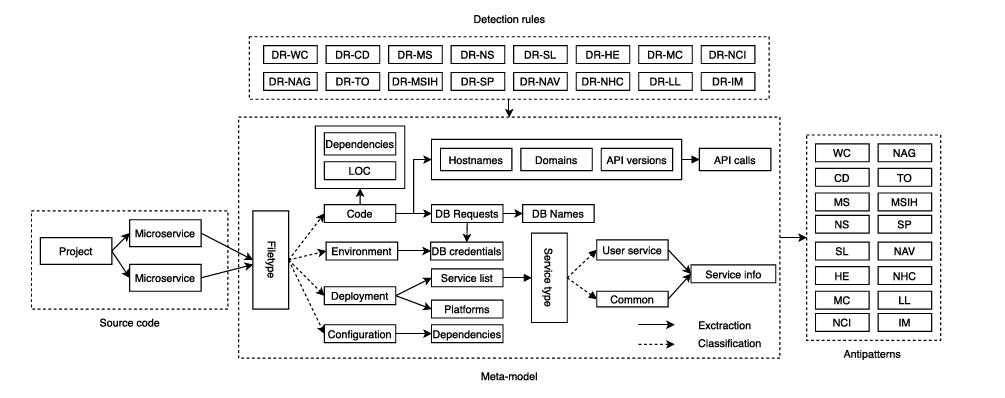
\includegraphics[width=\textwidth]
    {architetturaMARS.png}
    \caption{Microservice Antipatterns Research Software \cite{MARS}}
    \label{fig:architettura-mars}
\end{figure}

Il tool rileva un totale di 16 anti-patterns ed è stato testato dai ricercatori su un totale di 24 repository, confrontando i risultati ottenuti con una Ground Truth ottenuta mediante analisi manuale \cite{MARS}.
MARS è uno strumento totalmente automatizzato, il cui funzionamento si divide in tre fasi logiche e sequenziali: 
\begin{itemize}
    \item \textbf{Input}: Lo strumento riceve in input la repository Git o semplicemente la cartella locale nella sua interezza \cite{MARS}
    \item \textbf{Estrazione e Astrazione}: Estrapola le informazioni e le trasforma in una struttura dati standardizzati che prende il nome di \textbf{Metamodello} \cite{MARS}.
    \item \textbf{Rilevamento}: In questa fase, entrano in gioco gli algoritmi per la detection che lavorano sui dati forniti dal metamodello applicando delle regole statiche \cite{MARS}.
\end{itemize}

Il metamodello rappresenta il nucleo dell’intero tool: consente di “tradurre” tutte le informazioni raccolte in un linguaggio unico e uniforme, semplificando così la fase di rilevazione. In questo modo il tool interagisce direttamente con il metamodello, senza dover operare sul software analizzato \cite{MARS}.

Il metamodello è organizzato in diversi componenti che si occupano di immagazzinare informazioni in base al loro ambito di appartenenza:
\begin{itemize}
    \item \textbf{System}: È la radice dove è presente la repository nella sua interezza \cite{MARS}.
    Il System è costituito a sua volta da due elementi:
        \begin{itemize}
            \item \textit{Microservices}: Rappresenta un microservizio del sistema originale.
            \item \textit{Dependency}: Contiene le dipendenze del sistema o del singolo microservizio.
        \end{itemize}
    \item \textbf{Configuration}: Raccoglie i dati relativi ai file di configurazione statica \cite{MARS}.
    \item \textbf{Environment}: Memorizza i dati relativi alle variabili di ambiente \cite{MARS}.
    \item \textbf{Deployment}: Astrae informazioni sui file che servono a lanciare il sistema (es. Dockerfile) \cite{MARS}.
    \item \textbf{Code}: Contiene dati relativi al codice che viene scomposto in 5 parti: source files, imports, HTTP, database, call-graph (ottenuto mediante Understand \cite{scitools_understand}) \cite{MARS}.
\end{itemize}

\subsection{Funzionamento di MARS}

Il tool MARS opera secondo una logica di tipo
\textit{rule-based} \cite{MARS}. Una volta completata la fase di estrazione e costruito il metamodello, lo strumento non effettua inferenze semantiche sul dominio
applicativo né adotta tecniche di apprendimento automatico o analisi contestuale;
al contrario, applica un insieme di regole deterministiche predefinite che
mettono in relazione le informazioni raccolte con specifici criteri di
identificazione degli anti-pattern. Il comportamento del sistema è dunque
interamente guidato da euristiche esplicite, basate su confronti lessicali,
soglie numeriche, controlli strutturali e verifica della presenza o assenza
di determinati artefatti tecnici.

L'architettura osservata viene
rappresentata nel metamodello, mentre il modulo di detection confronta tale
rappresentazione con un insieme di condizioni considerate indicative di
potenziali criticità architetturali \cite{MARS}. Ciò rende il processo di rilevamento
trasparente e relativamente interpretabile, poiché ogni segnalazione può
essere ricondotta a una regola precisa e a uno specifico insieme di evidenze
estratte dal codice o dalla configurazione del sistema.

Più nel dettaglio, il funzionamento di MARS si fonda su quattro meccanismi
principali.

\begin{enumerate}
    \item \textbf{Analisi delle dipendenze.}  
    Una parte rilevante degli anti-pattern viene rilevata attraverso il
    confronto tra le dipendenze dichiarate dai microservizi e insiemi di
    dipendenze note. In questo caso MARS sfrutta le informazioni raccolte
    dall'Extractor nel metamodello, sia a livello di singolo servizio sia a
    livello di sistema, e verifica la presenza di librerie o framework ritenuti
    rappresentativi di determinate pratiche architetturali. Questo meccanismo
    è utilizzato, ad esempio, per anti-pattern quali \textit{Shared Libraries},
    \textit{No API Gateway}, \textit{No Health Check}, \textit{Local Logging},
    \textit{Insufficient Monitoring}, \textit{Manual Configuration} e
    \textit{Timeouts}. Nel caso di \textit{Shared Libraries},
    ad esempio, la regola confronta le dipendenze dei servizi e costruisce una
    mappa inversa dipendenza$\rightarrow$servizi, scartando preliminarmente
    quelle ritenute fisiologicamente comuni attraverso una blacklist dedicata \cite{madern2024_mars, MARS}.

    \item \textbf{Liste statiche di keyword e pattern.}  
    Un secondo meccanismo fondamentale è l'impiego di file di supporto esterni,
    costituiti da semplici liste testuali di token, estensioni, nomi di tool,
    pattern di file o parole chiave ricorrenti. Tali liste fungono da
    \textit{vocabolario operativo} della detection e vengono consultate dal
    detector durante l'applicazione delle regole. In questo senso, MARS non
    ``comprende'' semanticamente il significato architetturale di una libreria
    o di un file, ma riconosce corrispondenze lessicali tramite operazioni di
    \textit{pattern matching} o confronto per sottostringa. Questo approccio è
    impiegato, ad esempio, per identificare strumenti di
    \textit{service discovery}, gateway, framework di configurazione centralizzata,
    strumenti di CI/CD, librerie di monitoring o healthcheck, ma anche per
    filtrare nomi di servizi che non devono essere considerati ai fini di alcune
    analisi. Le liste statiche costituiscono quindi un elemento essenziale del
    comportamento di MARS, poiché definiscono in maniera esterna e configurabile
    il perimetro lessicale su cui si basano molte delle sue decisioni.
    La Tabella~\ref{tab:mars-txt-files} riassume i principali file di supporto utilizzati dal sistema per implementare le regole di detection descritte \cite{madern2024_mars}.

    \item \textbf{Soglie numeriche e regole quantitative.}  
    Alcuni anti-pattern sono rilevati non in base a parole chiave o dipendenze,
    ma tramite il confronto di metriche numeriche estratte dal sistema con soglie
    prefissate. In questa categoria rientrano soprattutto gli anti-pattern di
    natura dimensionale, come \textit{Nano Service} e \textit{Mega Service}.
    MARS calcola alcune grandezze aggregate a livello di sistema, come il numero
    totale di microservizi, le linee di codice complessive e le medie di LOC e file
    per servizio. Tali misure vengono poi utilizzate in modo euristico nelle regole
    di detection degli anti-pattern dimensionali: nel caso di \textit{Nano Service}
    il confronto avviene rispetto a soglie derivate dalla media di sistema, mentre
    per \textit{Mega Service} viene adottata una soglia fissa proporzionale al numero
    totale di LOC del sistema. Il vantaggio di questo approccio è la sua
    immediatezza: il rilevamento si basa su criteri quantitativi chiari e
    riproducibili. D'altra parte, si tratta di un'impostazione fortemente
    euristica, che non tiene conto del ruolo architetturale effettivo del servizio
    né della sua responsabilità funzionale \cite{madern2024_mars, MARS}.

    \item \textbf{Controlli diretti su file, configurazioni e artefatti di deployment.}  
    Un ulteriore meccanismo di detection consiste nell'ispezione diretta dei file
    presenti nel progetto. In questo caso l'Extractor individua file di
    configurazione, file sorgente (codice applicativo), file di ambiente, Dockerfile e altri artefatti
    rilevanti, registrandone i path nel metamodello; successivamente il detector
    utilizza tali informazioni per verificare condizioni specifiche. Questo avviene,
    ad esempio, nel caso di \textit{Manual Configuration}, dove vengono cercati
    file di configurazione locali e l'assenza di strumenti di configuration management riconosciuti tramite whitelist, oppure nel caso di \textit{Multiple Services per Host}, il detector utilizza indizi indiretti di deployment, come la presenza di file \texttt{docker-compose} a livello di sistema e l'assenza di Dockerfile dedicati per i singoli servizi.
    Analogamente, per \textit{No API Versioning} il detector apre direttamente i
    file di configurazione e cerca pattern lessicali nel loro contenuto testuale.
    Questo meccanismo evidenzia come MARS non si limiti a osservare metadati
    astratti, ma utilizzi anche evidenze concrete provenienti dal filesystem e
    dagli artefatti infrastrutturali del progetto. 
\end{enumerate}

Nel complesso, il funzionamento di MARS si basa sull'integrazione di questi
quattro meccanismi: le dipendenze descrivono l'ecosistema tecnologico del
servizio, le liste statiche definiscono il lessico di riferimento, le soglie
numeriche consentono di individuare anomalie dimensionali e i controlli su file
e configurazioni permettono di intercettare indizi infrastrutturali o
implementativi. L'approccio risultante è semplice, spiegabile e facilmente
estensibile, poiché nuove regole possono essere introdotte aggiungendo ulteriori
controlli e nuove liste di supporto. Al tempo stesso, esso rimane fortemente
dipendente dalla qualità dell'estrazione iniziale e dalla completezza dei file
statici utilizzati come base euristica per la detection.

\vspace{1em}
\begin{table}[H]
    \centering
    \scriptsize
    \renewcommand{\arraystretch}{1.2}
    \caption{File di configurazione utilizzati da MARS per la detection degli anti-pattern.}
    \label{tab:mars-txt-files}
    \resizebox{\textwidth}{!}{
    \begin{tabular}{| c | l | l | p{6.5cm} |}
        \hline
        \textbf{Anti-Pattern} & \textbf{File (.txt)} & \textbf{Tipo} & \textbf{Descrizione} \\ \hline
        
        \textbf{Nano Service} 
        & name\_ban\_for\_nano\_services & Blacklist nomi 
        & Lista di sottostringhe utilizzata per escludere servizi dal controllo dimensionale; se il nome contiene uno dei token, la detection del Nano Service viene ignorata. \\ \hline
        
        \multirow{2}{*}{\textbf{Wrong Cuts}} 
        & web\_extensions & Whitelist estensioni 
        & Estensioni considerate rappresentative di componenti frontend; il numero di file con tali estensioni viene confrontato con il totale per individuare servizi con forte componente di presentazione. \\ 
        & config\_extensions & Blacklist estensioni 
        & Estensioni escluse dal conteggio dei file perché non rappresentative della logica applicativa (es. configurazione, script o documentazione). \\ \hline
        
        \multirow{2}{*}{\textbf{Hardcoded Endpoints}} 
        & tlds & Lista TLD 
        & Lista di stringhe utilizzata per filtrare gli URL estratti dal codice; gli URL contenenti tali token vengono scartati come non rilevanti. \\ 
        & service\_discovery & Whitelist tool 
        & Pattern di tecnologie di service discovery utilizzati per verificare se gli endpoint sono risolti dinamicamente; la loro assenza, combinata con URL hardcoded, attiva la detection. \\ \hline
        
        \textbf{Shared Libraries} 
        & not\_shared\_dependencies & Blacklist dip. 
        & Insieme di pattern usato per escludere dipendenze comuni (framework o utility) dal confronto tra servizi durante la rilevazione di librerie condivise. \\ \hline
        
        \textbf{Manual Configuration} 
        & configuration & Whitelist tool 
        & Pattern di strumenti di configuration management utilizzati per verificare se i file di configurazione locali sono gestiti tramite sistemi centralizzati. \\ \hline
        
        \multirow{2}{*}{\textbf{No CI/CD}} 
        & cicd & Whitelist tool 
        & Pattern di strumenti CI/CD ricercati nelle dipendenze dei servizi per identificare pipeline di integrazione e distribuzione automatizzate. \\ 
        & cicd\_folders & Whitelist cartelle 
        & Nomi di directory tipiche di sistemi CI/CD usati per verificare la presenza di pipeline a livello di repository. \\ \hline
        
        \textbf{No API Gateway} 
        & gateway & Whitelist tool 
        & Pattern di tecnologie gateway ricercati nelle dipendenze; la loro assenza indica la mancanza di un punto di ingresso centralizzato. \\ \hline
        
        \textbf{Timeouts} 
        & circuit\_breaker & Whitelist tool 
        & Pattern di librerie di resilienza utilizzati per verificare la presenza di circuit breaker; la loro assenza, combinata con indizi di timeout nel codice, attiva la detection. \\ \hline
        
        \textbf{No Health Check} 
        & healthcheck & Whitelist tool 
        & Pattern di librerie che forniscono endpoint o meccanismi di health check; la loro assenza indica mancanza di verifica dello stato dei servizi. \\ \hline
        
        \textbf{Local Logging} 
        & logging & Whitelist tool 
        & Pattern di librerie di logging ricercati nelle dipendenze; utilizzati per determinare se esistono meccanismi di logging oltre il livello locale. \\ \hline
        
        \textbf{Insuff. Monitoring} 
        & monitoring & Whitelist tool 
        & Pattern di strumenti di monitoring e observability utilizzati per verificare la presenza di raccolta metriche e sistemi di osservabilità. \\ \hline
    \end{tabular}%
    }
\end{table}
\vspace{1em}


\subsection{Limitazioni di MARS}
Gli autori riconoscono che MARS presenta delle limitazioni:
\begin{itemize}
    \item \textbf{Dipendenze circolari}: MARS attualmente è in grado di rilevare se due microservizi dipendono l'uno dall'altro creando un ciclo chiuso (es. A chiama B, e B chiama A). Il problema nasce se il ciclo coinvolge più di 2 microservizi, in questo caso MARS non riesce a rilevarlo, presentando oggettive limitazioni della rilevazione \cite{MARS}.
    \item  \textbf{Logging e Monitoring}: MARS analizza il solo codice scritto dagli sviluppatori e non ha accesso alle infrastrutture su cui vengono fatte girare le applicazioni (come i cluster Kubernetes). Di conseguenza, se l'azienda gestisce i sistemi di monitoraggio e di log direttamente nell'infrastruttura senza scriverli nel codice, ciò genererà dei risultati errati \cite{MARS}.
    \item \textbf{Dimensioni}: stabilire se un servizio sia \textit{Nano} o \textit{Mega} è complesso e costringe MARS a basarsi su soglie euristiche definite a priori, che non sempre producono risultati ottimali \cite{MARS}.
    \item \textbf{Dipendenza da liste statiche}: 
    Come descritto in precedenza, la detection si basa fortemente su whitelist e blacklist
    definite manualmente. Sebbene tali liste rappresentino un meccanismo efficace,
    la loro configurazione e manutenzione risultano complesse e soggette a incompletezza,
    con il rischio di non riconoscere tecnologie non incluse o di generare falsi positivi
    in presenza di pattern troppo generici. 
    \item \textbf{Assenza di analisi semantica}: MARS si basa esclusivamente su regole e confronti lessicali, senza effettuare un'analisi semantica del codice o del comportamento del sistema. Di conseguenza,
    non è in grado di cogliere vincoli qualitativi o il reale ruolo architetturale
    dei servizi. Alcuni anti-pattern vengono quindi rilevati tramite euristiche
    semplificate, come nel caso di Nano e Mega Service, basati unicamente su metriche
    quantitative.

\end{itemize}

In conclusione, escludendo le problematiche relative ai singoli anti-pattern, MARS si configura come uno strumento che presenta limiti di utilizzabilità e richiede competenze adeguate per una corretta configurazione.

\section{Large Language Model}

I \textbf{Large Language Model (LLM)} sono dei modelli linguistici su larga scala, pre-addestrati su una grande mole di dati e basati su reti neurali \cite{llm_teoria}.
Questi modelli si basano sull'architettura \textbf{transformer}, un sofisticato framework di reti neurali che comprende un encoder e un decoder dotati di meccanismi di self-attention \cite{llm_teoria, Ghaderi2022Transformers}. Tale architettura permette agli LLM di elaborare e generare testo in modo efficiente, concentrandosi su diverse parti della sequenza di dati in input durante la fase di previsione \cite{llm_teoria, Ghaderi2022Transformers}. 
Tra i modelli più noti al grande pubblico rientrano GPT, Gemini, Claude e Qwen. In generale, gli LLM trovano applicazione in un ampio ventaglio di compiti, che spaziano dal recupero di informazioni alla comprensione e generazione del linguaggio naturale, configurandosi come strumenti avanzati in grado di rispondere a quesiti, sintetizzare contenuti e supportare processi decisionali in diversi contesti applicativi \cite{llm_teoria}.
Gli LLM nonostante i tanti pregi presentano alcune limitazioni: 
\begin{itemize}
    \item \textbf{Cut-off Date}: Gli LLM dispongono di informazioni solo fino alla data in cui sono stati addestrati e non vengono aggiornati ai dati più recenti in automatico. Pertanto, se vengono richieste informazioni successive a tale data, la precisione dell'output potrebbe essere compromessa \cite{llm_teoria}.
    \item \textbf{Hallucinations}: Si fa riferimento ad output, che pur sembrando corretti in termini grammaticali, sono di fatto errati in termini contenutistici, portando il modello a fornire risposte fuorvianti quando non dispone della risposta corretta \cite{llm_teoria}.
    \item \textbf{Long Training Times For Updates}: Riaddestrare il modello non è sempre una soluzione ottimale, poiché risulta essere un'attività computazionalmente onerosa.
\end{itemize}
Soluzioni che possono attenuare queste limitazioni sono:
\begin{itemize}
    \item \textbf{RAG}: La Retrival Augmented Generation è una tecnica avanzata di AI che permette di fornire al modello una base di conoscenza esterne, alla quale il modello può attingere \cite{llm_teoria}. In tal modo, il modello aggira il limite derivato dalle sue conoscenze attingendo ad un database esterno \cite{prompteng}.
    \item \textbf{Prompt Engineering}: Come vedremo nella Sezione~\ref{sec:prompteng}, ci sono una serie di tecniche mediante le quali possiamo guidare al meglio l'output dell'IA \cite{llm_teoria}.
    \item \textbf{Dati Contesto strutturati}: Fornire dati in ingresso ben elaborati e chiaramente formattati, può migliorare la precisione del modello.
\end{itemize}

\subsection{LLM come strumento di detection}
Come discusso in precedenza, i Large Language Models (LLM) eccellono nell'elaborazione e nell'estrazione di informazioni da testi complessi, rendendoli candidati promettenti anche come strumenti per il rilevamento di anomalie software. Tuttavia, l'attuale stato dell'arte evidenzia come il loro impiego sia fortemente sbilanciato verso l'identificazione di code smells a livello locale. Gli studi relativi al rilevamento di veri e propri anti-pattern architetturali, specialmente in ecosistemi a microservizi, risultano essere ancora in una fase nascente. Un esempio pionieristico in questa direzione è rappresentato dallo studio preliminare relativo a MicroPAD \cite{iac_llm}: in questa ricerca, gli autori propongono un approccio basato sugli LLM per analizzare artefatti di \textit{Infrastructure-as-Code} (IaC), come file Docker o configurazioni Terraform, al fine di individuare istanze di pattern architetturali a microservizi. Sebbene tale studio sia focalizzato sull'identificazione di pattern, piuttosto che di anti-pattern, esso dimostra concretamente la fattibilità di sfruttare i modelli linguistici e i file di configurazione per estrarre conoscenza architetturale da un sistema distribuito, suggerendo possibili sviluppi futuri anche verso la detection di difetti architetturali.


Le difficoltà nell'individuare AP architetturali sono le seguenti:
\begin{itemize}
    \item \textbf{Prospettiva locale vs prospettiva sistemica}: Nel caso dei \textit{code smells}, l'LLM valuta singoli moduli o porzioni di codice circoscritte. Al contrario, per individuare gli anti-pattern architetturali è necessaria una profonda comprensione del sistema nel suo complesso e delle interazioni tra i vari servizi, il che aumenta drasticamente la complessità dell'analisi.
    \item \textbf{Gestione della Context Window}: Sebbene i modelli di ultima generazione abbiano esteso notevolmente la propria finestra di contesto (arrivando a elaborare fino a milioni di token simultaneamente), saturare questa capacità comporta ancora delle criticità. Fornire in input moli di dati troppo ampie porta spesso a un degrado qualitativo dell'output e delle capacità di ragionamento del modello \cite{contextwindows_llm}. Nello specifico, si incorre nel noto fenomeno del "\textit{Lost in the Middle}" \cite{contextwindows_llm}, per cui l'LLM tende a ignorare o a recuperare con estrema difficoltà le informazioni posizionate nella parte centrale del prompt, privilegiando i dati all'inizio e alla fine.
     %A noi non succede mi verrebbe da dire.
    Di conseguenza, in compiti di \textit{detection} su interi repository, tale limitazione fisiologica comporta un inevitabile abbassamento della metrica di \textit{recall}.

    \item \textbf{Ambiguità interpretativa}: alcuni anti-pattern richiedono una componente interpretativa difficilmente riconducibile a sole regole quantitative. Ad esempio, nel caso di un \textit{mega-service}, non è sufficiente considerare esclusivamente il numero di LOC o di file, ma occorre valutare anche il dominio applicativo e il ruolo architetturale del servizio, che possono giustificarne o meno la dimensione.
\end{itemize}



\subsection{Prompt Engineering}
\label{sec:prompteng}
È una tecnica utilizzata per gli LLM, mediante la quale si utilizzano istruzioni testuali specifiche definite come \textit{"prompt"} per guidare il comportamento del modello e indirizzarlo verso la soluzione desiderata. In generale, con questo approccio possiamo evitare di modificare l'architettura interna o i parametri del modello \cite{prompteng}.

Possiamo definire alcune categorie di prompt:
\begin{itemize}
    \item \textit{Zero-Shot Prompting}: Il modello sfrutta unicamente la descrizione del prompt e fa affidamento sulle conoscenze acquisite in fase di pre-addestramento per generare una risposta \cite{prompteng}. Di conseguenza, il prompt non avrà a disposizione esempi o dimostrazioni \cite{prompteng_github}.

    \item \textit{Few-Shot Prompting}: A differenza del caso precedente, qui vengono forniti alcuni esempi pratici (input-output) all'interno del prompt per aiutare il modello a comprendere il formato e la richiesta logica \cite{prompteng}. 

    Questo tipo di approccio, migliora la risposta del modello ma utilizza molti più "token". Inoltre, si può condizionare il modello con pregiudizi presenti negli esempi scelti dall'utente \cite{prompteng}.

    \item \textit{Chain-of-Thought (CoT)}: Obbliga il modello a creare una catena di passaggi logici intermedi prima di fornire una risposta finale. Questo metodo aiuta il modello a superare le difficoltà nei ragionamenti complessi \cite{prompteng}.

    \item \textit{Auto CoT}: Risolve il problema del tempo necessario a creare manualmente esempi logici per il CoT. Utilizza frasi come "Pensiamo passo dopo passo" per spingere il modello a creare automaticamente le catene di ragionamento \cite{prompteng}.
\end{itemize}


Alla luce di queste limitazioni intrinseche e della mancanza di approcci consolidati in letteratura, risulta fondamentale definire una metodologia strutturata per la preparazione dei dati e l'interrogazione dei modelli. Il Capitolo successivo illustrerà nel dettaglio l'architettura 

dell'esperimento condotto in questa tesi, mostrando le strategie adottate (quali l'impiego di strumenti di aggregazione del codice e di Prompt Engineering avanzato) per mitigare le sfide appena esposte e valutare l'effettiva capacità degli LLM nel rilevamento degli anti-pattern architetturali.
%Controllata punteggiatura e errori di battitura 

\chapter{Esperimento}

\section{Goal dell'Esperimento}

Come evidenziato nel Capitolo~\ref{sec:capitolo4}, l’impiego dei Large Language Models (LLM) nel dominio dell’ingegneria del software si è concentrato prevalentemente sull’identificazione di \textit{code smells} e vulnerabilità locali. Sebbene studi recenti, come il prototipo MicroPAD, abbiano iniziato a dimostrare la fattibilità di utilizzare gli LLM per riconoscere pattern architetturali positivi a partire da file di configurazione (IaC), l’efficacia di tali modelli nel rilevamento di difetti complessi a livello di sistema distribuito, ovvero gli anti-pattern architetturali nelle architetture a microservizi (MSA), analizzando l’intera \textit{codebase}, rappresenta un ambito di ricerca ancora largamente inesplorato.

Alla luce di queste mancanze, l'obiettivo principale del presente esperimento è valutare empiricamente le capacità e i limiti degli LLM di ultima generazione nell'individuare specifici AP (sia architetturali sia appartenenti ad altre categorie) all'interno di \textit{codebase} reali di grandi dimensioni.

%Le lascio in inglese?
Nello specifico, l'esperimento è stato progettato per rispondere alle seguenti \textit{Research Questions (RQ)}:
\begin{itemize}
    \item \textbf{RQ1: Quanto sono efficaci gli LLM nel rilevare gli anti-pattern nelle MSA?}

    L'obiettivo è misurare l'efficacia pura dei modelli nel riconoscere difetti architetturali, fornendo in ingresso un input elaborato mediante \textit{Repomix} e valutando l'output analizzando metriche standard, come Precision, Recall e F1, rispetto a una \textit{ground truth} validata manualmente.
    
    \item \textbf{RQ2: Come si confrontano gli LLM con gli strumenti di analisi statica allo stato dell’arte per il rilevamento degli anti-pattern nelle MSA?}

    Successivamente, l'esperimento si propone di confrontare criticamente le performance ottenute dagli LLM con quelle prodotte da strumenti di detection considerati lo stato dell'arte in questo dominio. In particolare, i risultati dei modelli verranno comparati con quelli generati da MARS, al fine di comprendere se l'approccio degli LLM possa superare, eguagliare o quantomeno complementare i limiti strutturali tipici di tali strumenti.

\end{itemize}
Per raggiungere questi obiettivi, lo studio prevede l'esecuzione di test comparativi su un set eterogeneo di repository open-source, impiegando tecniche avanzate di \textit{Prompt Engineering} e strumenti di gestione dei dati di input (come \textit{Repomix}) per ridurre le problematiche associate alla dimensione del contesto e alla sua elaborazione.

\subsection{Selezione degli LLM}

Per condurre l'esperimento sono stati selezionati tre modelli nel panorama attuale: \textbf{Qwen 3.5 Plus} \cite{alibaba2026qwen35}, \textbf{Gemini 3.0 Pro} \cite{deepmind2026gemini31} e \textbf{ChatGPT 5.2} \cite{openai2025gpt52}. La scelta di questi specifici modelli è stata guidata principalmente da un requisito tecnico fondamentale, necessario per affrontare le complessità dell'analisi architetturale: la \textbf{gestione di finestre di contesto estese (\textit{Large Context Windows})}.

Come analizzato nel Capitolo~\ref{sec:capitolo4}, l'analisi di un'architettura a microservizi richiede l'ingestione di interi repository. I modelli selezionati dispongono di capacità di elaborazione molto elevate, che consentono di processare l'intera \textit{codebase} senza ricorrere a complessi e potenzialmente rischiosi meccanismi di frammentazione del codice. Nello specifico, come riassunto nella Tabella~\ref{tab:llm-selection}, Gemini e Qwen offrono una finestra di contesto pari a 1.000.000 di token, mentre ChatGPT 5.2 supporta contesti fino a 400.000 token. Durante i test empirici, tali dimensioni si sono mostrate generalmente adeguate all'elaborazione di progetti di grandi dimensioni, senza errori espliciti o interruzioni del servizio.

Va inoltre osservato che, nel caso di ChatGPT, ai limiti della finestra di contesto del modello si affiancano vincoli propri della piattaforma di caricamento dei documenti: i file di testo e i documenti caricati in una conversazione o in un GPT sono soggetti a un limite di 2 milioni di token per file, oltre al limite dimensionale di 512 MB \cite{openai_file_uploads_faq}. Tale soglia costituisce quindi un vincolo pratico all'ingestione di repository o documentazione particolarmente estesi, distinto dalla finestra di contesto effettivamente disponibile al modello \cite{openai_file_uploads_faq}.

Durante i test empirici, si è tuttavia osservata un'eccezione metodologicamente rilevante: per tre repository analizzati, lo strumento di aggregazione del codice (Repomix \cite{repomix2026}) ha stimato un peso in token nominalmente superiore alla soglia dei 400.000 token attribuita a ChatGPT 5.2. Nonostante ciò, il modello ha processato l'input senza restituire errori espliciti di superamento del limite di contesto. Tale risultato va interpretato con attenzione. In primo luogo, la stima fornita da Repomix ha carattere approssimativo e può non coincidere con il conteggio effettivo dei token operato dal sistema. In secondo luogo, l'assenza di errori visibili non consente di escludere che il modello abbia adottato strategie interne non osservabili per la gestione dell'input, con possibili effetti sulla completezza dell'elaborazione. Di conseguenza, pur in assenza di fallimenti espliciti, non può essere esclusa una perdita informativa.

La Tabella~\ref{tab:llm-selection} riassume le specifiche tecniche principali dei tre modelli scelti.

\begin{table}[H]
    \centering
    \caption{Lista LLM utilizzati.}
    \label{tab:llm-selection}
    \vspace{0.2cm}
    \renewcommand{\arraystretch}{1.3}
    \resizebox{\textwidth}{!}{%
    \begin{tabular}{l l c}
        \toprule
        \textbf{Modello} & \textbf{Sviluppatore} & \textbf{Context Window (Token)} \\
        \midrule
        \textbf{Gemini 3.0 Pro} & Google DeepMind & 1.000.000 \\
        \textbf{Qwen Plus 3.5}  & Alibaba Cloud   & 1.000.000 \\
        \textbf{ChatGPT 5.2}    & OpenAI          & 400.000 \\
        \bottomrule
    \end{tabular}%
    }
\end{table}

\subsection{Repository analizzate}

Per valutare l'efficacia degli LLM nell'identificazione degli anti-pattern, è stato selezionato un dataset composto da 13 repository \textit{open-source} basate su architettura a microservizi. Tale dataset, le cui metriche dimensionali sono riassunte nella Tabella~\ref{tab:repositories}, è caratterizzato da un'elevata eterogeneità: comprende infatti sia progetti dimostrativi di piccole dimensioni (poche centinaia di linee di codice), sia sistemi complessi assimilabili a contesti \textit{enterprise} (con decine di microservizi e quasi 90.000 linee di codice, come nel caso di \textit{Micro Company} e \textit{Lakeside Mutual}).

\begin{table}[H]
    \centering
    \caption{Elenco delle repository a microservizi analizzate nell'esperimento, con le relative metriche dimensionali.}
    \label{tab:repositories}
    \vspace{0.2cm}
    \renewcommand{\arraystretch}{1.2}
    \resizebox{\textwidth}{!}{%
    \begin{tabular}{l c c c c}
        \toprule
        \textbf{Repository} & \textbf{Microservices} & \textbf{Files} & \textbf{LOC} & \textbf{Reference} \\
        \midrule
        Apollo & 9 & 68 & 29.510 & \cite{ApolloRepository} \\
        TeaStore & 3 & 62 & 5.073 & \cite{TeaStoreRepository} \\
        Spring Cloud Microservice Movie & 4 & 33 & 885 & \cite{SpringCloudMicroserviceMovieRepository} \\
        Freddy's BBQ & 6 & 35 & 1.752 & \cite{FreddysBBQRepository} \\
        Piggymetrics & 4 & 88 & 3.176 & \cite{PiggymetricsRepository} \\
        FTGO & 9 & 257 & 8.239 & \cite{FTGORepository} \\
        Spring Boot Microservices & 2 & 4 & 116 & \cite{SpringBootMicroservicesRepository} \\
        Lakeside Mutual & 9 & 424 & 89.477 & \cite{LakesideMutualRepository} \\
        Warehouse Microservice & 6 & 222 & 4.623 & \cite{WarehouseMicroserviceRepository} \\
        Qbike & 5 & 77 & 2.057 & \cite{QbikeRepository} \\
        Microservice Demo & 3 & 38 & 1.766 & \cite{MicroserviceDemoRepository} \\
        CQRS Microservice Sampler & 3 & 26 & 1.028 & \cite{CQRSMicroserviceSamplerRepository} \\
        Micro Company & 17 & 244 & 90.315 & \cite{MicroCompanyRepository} \\
        \bottomrule
    \end{tabular}%
    }
\end{table}

\subsection{Ground truth manuale}
A tale scopo, per le tredici repository selezionate è stata utilizzata la ground truth (GT) manuale resa disponibile dallo studio MARS \cite{MARS}. È importante precisare che tale ground truth non è stata generata automaticamente dal tool MARS, bensì costruita manualmente dagli autori dello studio attraverso un processo di validazione umana. 
MARS utilizza il GT come strumento di validazione del proprio output.
I dati completi relativi alla \textit{Ground Truth} sono pubblicamente accessibili e consultabili al riferimento \cite{GT_mars}.

\section{Procedura sperimentale}

Come illustrato nel diagramma in Figura~\ref{fig:pipeline}, l'architettura dell'esperimento è stata formalizzata in un processo sistematico e riproducibile. L'esecuzione si articola in quattro fasi, che rispecchiano l'esatta evoluzione cronologica dello studio: dall'analisi degli LLM fino al successivo confronto con MARS.

\vspace{0.8em}
\begin{figure}[ht]
    \centering
    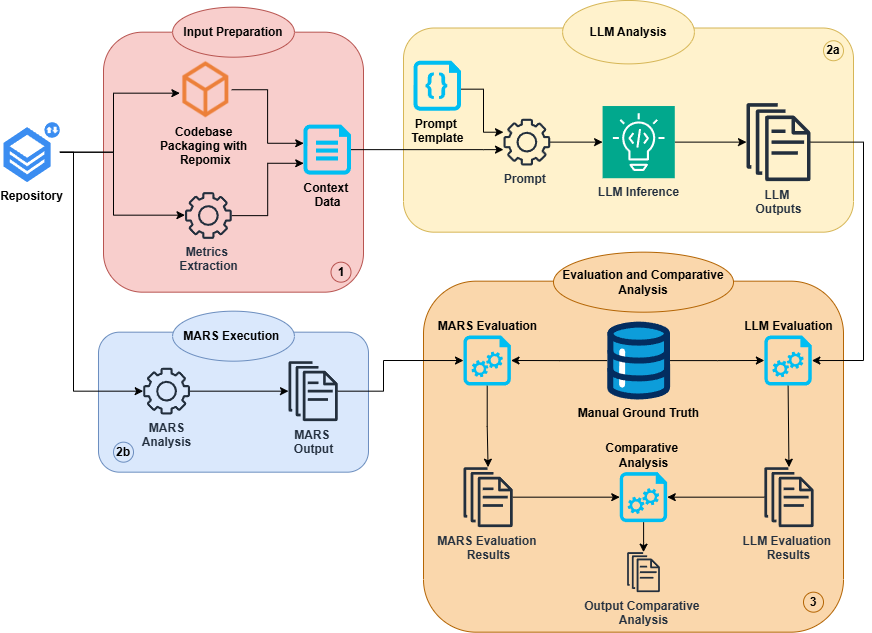
\includegraphics[width=1.0\textwidth]{img/pipeline_d2.png}
    \caption{Pipeline dell'esperimento.}
    \label{fig:pipeline}
\end{figure}

Di seguito si riportano le varie fasi della pipeline dell'esperimento:
\begin{description}
    \item[Fase 1: Input Preparation]
    \hfill \\
    In questa fase, è fornito in input a \textit{Repomix} e allo script di estrazione delle metriche quantitative la repository selezionata. 
    Mediante \textit{Repomix} incapusuliamo la repository con una struttura LLM-friendly, generando un unico artefatto testuale ottimizzato. 
    Parallelamente è eseguita la sotto-fase di \textit{Metrics Extraction} mediante la quale con uno script Python, si vanno ad estrarre i parametri quantitativi (es. LOC, numero di file e di servizi). 
    I due output delle due sotto-fasi generano i \textit{Context Data}, ovvero la base di conoscenza sulla quale il modello dovrà ragionare per rilevare gli anti-pattern. 
    
    \item[Fase 2a: LLM Analysis]
    \hfill \\
    I \textit{Context Data} sono combinati al \textit{Prompt Template} per generare il \textit{Prompt} finale che verrà sottoposto ai modelli. 
    Il \textit{Prompt Template} ha in generare una struttura fissa; per ciascun anti-pattern cambiano esclusivamente la definizione, l'esempio e quando necessario, alcune \textbf{regole aggiuntive} specifiche dell'AP analizzato.
    Realizzato il \textit{Prompt}, si procede alla sotto-fase di \textit{LLM Inference}, nella quale i tre modelli selezionati (ChatGPT, Gemini e Qwen) elaborano l'input fornito generando gli \textit{LLM Outputs} della detection.

    
    \item[Fase 2b: MARS Execution]
    \hfill \\
    Parallelamente al processo visto nelle prime due fasi, viene eseguito il tool di analisi statica MARS, generando la baseline necessaria per il confronto con gli output dei modelli.

    \hfill \\
    \item[Fase 3: Evaluation and Comparative Analysis]
    \hfill \\
    Gli output degli LLM sono successivamente analizzati nella sotto-fase di \textit{LLM Evaluation}, nella quale si confrontano i risultati ottenuti con una \textit{Manual Ground Truth} per ottenere di fatto delle metriche qualitative (\textit{Precision} \textit{Recall} \textit{F1-score}) mediante le quali possiamo comprendere a pieno quanto i modelli sono precisi e di conseguenza rispondere alla \textbf{prima RQ}.
    Analogamente a quanto fatto con gli LLM, nella sotto-fase di \textit{MARS Evaluation} vengono valutati i risultati di ottenuti da MARS. 
    Ottenute le metriche qualitative riferite agli output degli LLM e di MARS, si può procedere al confronto diretto tra i due approcci, ottenendo di conseguenza risposta alla \textbf{seconda RQ}.
\end{description}

Nel seguito vengono approfondite alcune sotto-fasi del processo, al fine di chiarire in modo puntuale le modalità con cui sono stati ottenuti i risultati che saranno oggetto di discussione più avanti.

\subsection{Incapsulamento repository con Repomix (Fase 1)}

In una fase preliminare dell'esperimento, si è cercato di fornire agli LLM una rappresentazione astratta dell'architettura. Per farlo, sono stati testati strumenti open-source di analisi statica come \textit{code2dfd} e \textit{rad-source}, con l'obiettivo di estrarre diagrammi di flusso dei dati (DFD) e grafi delle dipendenze \cite{Static_Tool, cloudhubs_rad_source, Code2DFD23}. Tuttavia, questa strategia ha mostrato due limiti principali.

In primo luogo, ciascuno strumento catturava soltanto uno specifico sottoinsieme di informazioni, restituendo quindi una rappresentazione inevitabilmente parziale del sistema. Tale limite non consentiva di includere tutti gli elementi necessari per individuare anti-pattern legati a configurazioni o logiche di comunicazione inter-servizio. In secondo luogo, per avere una visione completa che fosse idonea per ogni AP, sarebbe stato necessario usare più strumenti contemporaneamente, introducendo un ulteriore livello di complessità per normalizzare e unire output molto diversi in un unico file per l'LLM.

Per evitare questa frammentazione, si è deciso di sfruttare l'ampia finestra di contesto dei modelli moderni per fornire in input l'intera \textit{codebase}. È stato quindi adottato \textbf{Repomix}, uno strumento open-source progettato per aggregare l'intero contenuto di una repository software in un singolo file di testo, strutturato appositamente per essere compreso dai \textit{Large Language Models} \cite{repomix2026}.

L'uso di Repomix è stato guidato da un file di configurazione personalizzato (\texttt{repomix.config.json}) per ottimizzare il testo ed escludere il codice non rilevante per l'analisi architetturale \cite{repomix2026}. Nello specifico, sono state applicate queste regole \cite{repomix2026}:

\begin{itemize}
    \item \textbf{Pulizia del codice:} sono stati rimossi i commenti e le righe vuote (\texttt{removeComments: true}, \texttt{removeEmptyLines: true}) per massimizzare la densità delle informazioni. Questa scelta è stata motivata anche dalla necessità di garantire un confronto equo. I commenti, infatti, possono contenere suggerimenti preziosi sulle scelte architetturali che agevolerebbero il modello; tuttavia, non essendo presenti in egual misura in tutti i progetti, lasciarli intatti avrebbe introdotto un \textit{bias} valutativo, alterando le prestazioni di \textit{detection} (migliori o peggiori) in base al livello di documentazione interna della singola \textit{codebase}.
    
    \item \textbf{Numerazione delle righe:} è stata attivata l'opzione per mostrare i numeri di riga (\texttt{showLineNumbers: true}), fondamentale per permettere all'LLM di indicare con precisione in quale file e a quale riga si trova un potenziale anti-pattern. Inoltre, tale funzione si è rivelata utile per controllare in maniera manuale alcuni risultati, potendo rintracciare facilmente gli artefatti all'interno della codebase.
    
    \item \textbf{Esclusioni mirate:} invece di usare le regole base del sistema di controllo di versione (\texttt{useGitignore: false}), è stata definita una lista personalizzata dei file da ignorare mediante l'opzione  (\texttt{customPatterns}). Oltre a file binari, librerie esterne (es. \texttt{node\_modules}) e documentazione, sono state escluse interamente le suite di \textbf{testing} (directory \texttt{tests/}, file \texttt{*Test.java}, ecc.). I file di test non contengono la logica strutturale dei microservizi; pertanto, la loro esclusione ha permesso di risparmiare una grande quantità di spazio, facilitando il lavoro di elaborazione dei modelli.
    Il file di configurazione utilizzato per Repomix è reperibile al seguente riferimento \cite{barbato_tesi_llm_scripts}.
    
    
\end{itemize}

Il file finale è stato generato in formato testo semplice (\texttt{style: "plain"}) mantenendo intatta la struttura delle directory (\texttt{directoryStructure: true}), per aiutare il modello a orientarsi tra i vari moduli e capire come sono separati i microservizi.

Infine, per quanto riguarda il consumo di spazio, Repomix include una funzione di stima dei \textit{token}. Nel file di configurazione è stato impostato l'algoritmo di codifica \texttt{o200k\_base} (lo standard utilizzato dai modelli OpenAI più recenti). È importante precisare che i tre modelli scelti per l'esperimento (ChatGPT, Gemini e Qwen) utilizzano \textit{tokenizer} proprietari differenti e quindi calcolano i \textit{token} in modo leggermente diverso l'uno dall'altro. Tuttavia, l'uso dello standard OpenAI è servito unicamente come metrica di stima di riferimento: ha permesso di verificare rapidamente che la dimensione totale del file generato per ogni repository fosse ampiamente contenuta all'interno della grande finestra di contesto (fino a 1 milione di \textit{token}) supportata da tutti i modelli in fase di inferenza.
Nei rari casi in cui la dimensione della repository eccedeva i limiti del modello, non sono stati osservati cali percepibili nelle prestazioni di detection. Questo risultato suggerisce che, nel setup sperimentale adottato, il sistema abbia gestito input di grandi dimensioni senza manifestare errori espliciti, pur senza consentire conclusioni definitive sui meccanismi interni di elaborazione. Tuttavia, tale interpretazione è basata esclusivamente su evidenze empiriche e non su dettagli implementativi esplicitamente documentati.

\subsection{Estrazione metriche (Fase 1)}

L'output testuale generato da Repomix offre una visione completa della \textit{codebase}, ma lo strumento non fornisce la possibilità di effettuare il calcolo e l'aggregazione di metriche strutturali relative alla repository, come il numero esatto di righe di codice, classi o metodi raggruppati per singolo microservizio. D'altra parte, richiedere a un LLM di ricavare tali informazioni direttamente dal file generato da repomix risulta essere complesso e aumenterebbe inutilmente il carico in termini computazionali del modello.

Poiché l'identificazione di anti-pattern dimensionali, come il \textit{MegaService} o il \textit{NanoService}, richiede soglie numeriche precise, si è scelto di alleggerire il compito del modello fornendogli dati già pre-calcolati. Di conseguenza, parallelamente all'esecuzione di Repomix, è stato sviluppato uno script Python custom incaricato di eseguire un'analisi statica leggera; il codice sorgente completo dello strumento è disponibile nel repository GitHub del progetto \cite{barbato_tesi_llm_scripts}. L'obiettivo dello \textit{script} è estrarre metriche software oggettive per ciascun microservizio e restituirle in un formato strutturato (\texttt{JSON}).

Il funzionamento dello \textit{script} si articola in due macro-operazioni principali:

\vspace{0.5em}
\noindent\textbf{1. Rilevamento dinamico dei microservizi (\textit{Service Discovery})}\\
Lo \textit{script} analizza la struttura della \textit{codebase} alla ricerca di file di configurazione tipici dei vari ecosistemi di sviluppo (ad esempio \texttt{pom.xml} per Maven, \texttt{build.gradle} per Gradle, \texttt{package.json} per frontend/Node.js e \texttt{go.mod} per Go). Questa logica consente di identificare automaticamente i confini di ciascun servizio, escludendo i file di aggregazione generale, come i POM aggregatori.
Di seguito si riporta un estratto della logica di rilevamento:

\vspace{0.5em}
\noindent\textit{Codice 1: Frammento per il rilevamento dinamico dei microservizi.}
\begin{Verbatim}[breaklines=true, breakanywhere=true]
def find_microservices(project_root: Path):
    services = {}
    # Rilevamento Maven (escludendo i pom aggregatori)
    for pom in project_root.rglob("pom.xml"):
        if not is_excluded_path(pom) and not is_aggregator_pom(pom):
            add_service(pom.parent, "maven")
            
    # Rilevamento Node/Frontend (evitando i node_modules)
    for pkg in project_root.rglob("package.json"):
        if not is_excluded_path(pkg) and "node_modules" not in pkg.parts:
            add_service(pkg.parent, "node")
            
    # Rilevamento Go, Python, Docker...
    return services
\end{Verbatim}
\vspace{0.5em}

\noindent\textbf{2. Conteggio robusto delle metriche (LOC, Classi, Metodi)}\\
Una volta delimitati i servizi, lo \textit{script} calcola le metriche dimensionali. Per garantire l'accuratezza delle \textit{Lines of Code} (LOC), è stato implementato un \textit{parser} in grado di ignorare le righe vuote e i commenti (sia in linea sia a blocco), supportando sintassi eterogenee (stile C, HTML e Hash). Lo strumento utilizza inoltre espressioni regolari per contare il numero di classi, metodi e costruttori definiti nel codice, discriminando tra i vari linguaggi di programmazione supportati (Java, Kotlin, Python, Go, TypeScript/JavaScript). È stata inoltre integrata una logica per evitare il doppio conteggio nei casi di microservizi annidati (\textit{cross-service exclusion}).


\vspace{0.5em}
L'output finale di questo processo è un file \texttt{.json}  che racchiude tutte le informazioni necessarie per ogni microservizio individuato (come i totali di LOC, classi e metodi). È importante osservare che il file in questione non viene fornito al modello per ogni AP. Al fine di ottimizzare l'analisi, si è preferito fornire al modello lo stretto necessario e di conseguenza tale file viene aggiunto ai \textbf{Context Data (3a)} solo per gli AP dimensionali (\textit{NanoService} e \textit{MegaService}).

Per la rilevazione di tutti gli altri AP, il modello si basa unicamente sul codice sorgente compattato, evitando di sovraccaricare il \textit{prompt} con metriche numeriche non pertinenti al \textit{task} specifico.

\subsection{Costruzione del Prompt e Input al Modello (Fase 2a)}
\vspace{1em}
Per garantire la totale riproducibilità dell'esperimento e standardizzare le risposte, è stato ingegnerizzato un \textit{Template} base da cui sono stati derivati i singoli \textit{prompt}. Come si evince dal seguente schema strutturale, le istruzioni, i vincoli di rilevamento e i formati di \textit{output} sono stati mantenuti rigorosamente identici per tutte le esecuzioni, variando esclusivamente la definizione teorica del difetto ricercato.

\vspace{1em}
\noindent\textit{Codice 3: Struttura base del Prompt Template utilizzato per le inferenze.}
\vspace{0.5em}

\begin{mdframed}[linewidth=0.8pt, innermargin=10pt, outermargin=0pt]
\sffamily \small \raggedright
Act as an expert microservice architecture analyst and reverse-engineering researcher tasked with detecting a specific Architectural Anti-Pattern in a provided software repository or codebase.\\

You will receive one or more input files describing a software system. Treat these inputs as the sole source of truth; do not assume the presence of any missing files or behaviors. Never respond with UNKNOWN.\\

Your task is to analyze the entire provided artifacts and determine whether the specified microservice architectural anti-pattern is \textbf{PRESENT} or \textbf{ABSENT}, strictly according to the exact definition and example given below.\\

\vspace{0.5em}
\textbf{ANTI-PATTERN}\\
\textbf{Name:} [NOME ANTI-PATTERN]\\
\textbf{Definition:} [DEFINIZIONE FORMALE DELL'AP]\\
\textbf{Example:} [ESEMPIO DESCRITTIVO OPPURE BASATO SU INPUT/OUTPUT]\\

\vspace{0.5em}
\textbf{Detection Constraints:}\\
- Follow only the provided definition and example without generalization or extension.\\
- Translate the definition into observable indicators only if explicitly implied.\\
- Cross-reference all provided inputs including services, modules, endpoints, dependencies, shared resources, and deployment descriptors.\\
- If any required information is missing, ambiguous, or unverifiable from the artifacts, output \textbf{ABSENT} and specify exactly what is missing.\\
- The anti-pattern name in your output must exactly match the provided Name.\\

\vspace{0.5em}
\textbf{Reasoning Instructions:}\\
- Think carefully and exhaustively, based solely on the provided definition and example.\\
- Do not reveal your internal reasoning steps or intermediate thoughts.\\

\vspace{0.5em}
\textbf{Output Format (ONLY these sections, in this order, with no additional content):}\\

\textbf{ANTI-PATTERN:} [Exact Name]\\
\textbf{STATUS:} PRESENT | ABSENT\\

\vspace{0.5em}
\textbf{SUMMARY (1-2 lines):}\\
- \textbf{PRESENT:} Briefly describe what the anti-pattern is and where it manifests.\\
- \textbf{ABSENT:} Briefly explain why the analyzed artifacts do not meet the definition or example.\\

\vspace{0.5em}
\textbf{RATIONALE (max 4 bullets):}\\
- \textbf{PRESENT:} Reasons why observed features match the definition/example; key indicators.\\
- \textbf{ABSENT:} Which required conditions are not met or unverifiable from the artifacts.\\

\vspace{0.5em}
\textbf{SUPPORTING INDICATORS (only if PRESENT):}\\
- Provide 1 to 4 concrete observations anchored to specific artifacts (including filename and line number if available).\\
- Additional relevant observations as necessary.\\

\vspace{0.5em}
\textbf{SERVICES / COMPONENTS INVOLVED:}\\
- \textbf{PRESENT:} Explicitly list affected services or components identifiable from the artifacts.\\
- \textbf{ABSENT:} None identified.\\

\vspace{0.5em}
Ensure clarity, precision, and strict adherence to the instructions throughout.
\end{mdframed}
\vspace{1em}

\vspace{1em}

Per la costruzione dei \textit{prompt}, si è scelto di combinare diverse tecniche con l'obiettivo di guidare i modelli in modo preciso, evitando di condizionarne le scelte o di introdurre involontariamente dei \textit{bias} durante l'analisi:

\begin{itemize}
    \item \textbf{Role Prompting:} Chiedere all'LLM di agire come un esperto (\textit{"Act as an expert microservice architecture analyst..."}) lo aiuta a calarsi nel giusto contesto, spingendolo ad adottare il rigore tipico di un ingegnere del software.
    
    \item \textbf{Zero-shot ancorato a definizione ed esempio:} il prompt utilizzato prevede che il modello si basi e faccia fede solo alle informazioni derivate dalla \textit{definizione} e dall'\textit{Example} per la detection. Sono stati usati \textit{Example} descrittivi e narrativi (come lo scenario di un \textit{e-commerce}) con l'aggiunta, in alcuni casi, di alcuni frammenti di codice per aiutare il modello nell'identificazione sintattica di alcuni AP. 
    Si specifica che per alcuni \textit{prompt} la presenza della sezione \textit{Example} non portava a reali vantaggi; di conseguenza, per alleggerire il testo, in questi casi è stata omessa.
    
    \item \textbf{Constraint-Based Prompting:} Serve a "ingabbiare" il comportamento del modello per evitare risposte imprevedibili o formattazioni sballate. Abbiamo usato vincoli strutturali rigidi (come \textit{"Never respond with UNKNOWN"} e una precisa struttura per l'\textit{output}).
    
    \item \textbf{Rule-Based Prompting:} È stato utilizzato in modo molto mirato senza eccedere per gestire specifiche eccezioni di dominio. L'obiettivo non era pilotare il modello passo dopo passo, ma fornirgli solo i confini essenziali su cosa escludere a priori (ad esempio, i file di test o i componenti infrastrutturali). Questo ha permesso di evitare i falsi positivi più banali, lasciando comunque all'LLM la massima libertà e autonomia nell'individuare i difetti veri e propri.
    
    \item \textbf{Chain-of-Thought (CoT):} Abbiamo chiesto al modello di ragionare a fondo prima di decidere, ma di tenere per sé i passaggi intermedi (\textit{"Do not reveal your internal reasoning steps"}). In questo modo otteniamo un'analisi profonda senza "sporcare" il testo finale generato.
    
\end{itemize}

La totalità dei prompt utilizzati è consultabile al riferimento \cite{barbato_tesi_llm_scripts}.

\vspace{1em}
\subsubsection*{Selezione delle definizioni e regole}
Un passaggio importante ha riguardato la scelta delle definizioni degli anti-pattern. Le definizioni formali proposte nel \textit{paper} originale di Cerny et al. risultavano a volte troppo stringenti o complesse per essere recepite correttamente da un LLM, con conseguente abbassamento della recall. Per agevolare il compito del modello, in alcuni casi abbiamo preferito utilizzare le definizioni fornite dal \textit{paper} di MARS, che si sono rivelate più pratiche e dirette. La \textbf{Tabella~\ref{tab:ap_definitions}} riassume le definizioni esatte usate per ogni anti-pattern e la loro provenienza bibliografica.

\begin{table}[H]
    \centering
    \scriptsize
    \renewcommand{\arraystretch}{1.3}
    \caption{Definizioni degli Anti-Pattern utilizzate nei Prompt.}
    \label{tab:ap_definitions}
    \begin{tabular}{| p{3cm} | p{8.5cm} | p{3cm} |}
        \hline
        \textbf{Anti-Pattern} & \textbf{Definizione fornita al Modello} & \textbf{Fonte} \\ \hline
        
        \textbf{Wrong Cuts} & The system is decomposed into microservices following technical aspects, such as the presentation layer, business layer, and data access layer. Microservice should encapsulate functionalities fulfilling a single purpose. & Cerny et al. \cite{CernyCatalogo} \\ \hline

        \textbf{Nano-Service} & The service is too fine-grained and only has a few operations. Its overhead (communications, maintenance, and so on) outweighs its utility. Nanoservices cause fragmented logic and performance issues. & Cerny et al. \cite{CernyCatalogo} \\ \hline

        \textbf{Shared Libraries} & Microservices should not share runtime libraries or source code that contain business logic or domain-specific functionality. Sharing such internal libraries breaks service boundaries and reduces independence. & Cerny et al. \cite{CernyCatalogo} \\ \hline

        \textbf{Hardcoded \newline Endpoint} & Microservice IP addresses, ports, or full endpoint URLs are explicitly specified in source code, configuration files, or environment variables in a way that couples clients to a specific address/port. & Cerny et al. \cite{CernyCatalogo} \\ \hline

        \textbf{Manual \newline Configuration} & Configuration of instances, services, and hosts is done manually. Microservices should separate the core codebase from the configuration management to enable automation. & Cerny et al. \cite{CernyCatalogo} \\ \hline

        \textbf{No API Gateway} & When a microservice-based system lacks an API gateway, the clients of the application necessarily have to invoke its microservices directly. The system lacks a unified entry point for centralized routing. & Cerny et al. \cite{CernyCatalogo} \\ \hline

        \textbf{Mega-Service} & Microservices should be small, independent, independently deployable units and serve a single purpose. A mega service has a high number of lines of code, modules, or files, as well as a high fan-in. & Cerny et al. \cite{CernyCatalogo} \\ \hline

        \textbf{Shared \newline Persistency} & Different microservices are accessing the same database/schema (often the same tables/entities). In the worst kind, different services use the same entities of a service. & Cerny et al. \cite{CernyCatalogo} \\ \hline

        \textbf{No API \newline Versioning} & In a microservice architecture, if one or more services expose REST APIs to clients without any form of versioning (path-based, header-based, or query parameter), then the system suffers from this. & Cerny et al. \cite{CernyCatalogo} \\ \hline

        \textbf{No Health Check \newline (NHC)} & This antipattern describes microservices that are not periodically health-checked. Unavailable microservices may not be noticed, leading to timeouts and other errors. & MARS \cite{MARS} \\ \hline

        \textbf{Insufficient \newline Monitoring} & Performance and failure of the microservices are not tracked. Failures become more difficult to catch and tracking performance issues become more tedious. A solution is to adopt a global monitoring tool. & Cerny et al. \cite{CernyCatalogo} \\ \hline

        \textbf{Timeouts \newline (TO)} & This antipattern happens when timeout values are set and hard-coded in HTTP requests, which leads to unnecessary disconnections or delays. & MARS \cite{MARS} \\ \hline

        \textbf{Multiple Service \newline Instances Per Host} & A single host contains multiple microservices instances deployed to the same host. Microservices have to share the same resources that are available inside the host. & Cerny et al. \cite{CernyCatalogo} \\ \hline

        \textbf{Local Logging \newline (LL)} & This antipattern results from microservices having their own logging mechanism, which prevents aggregation and analyses of their logs and the monitoring and recovery of systems. & MARS \cite{MARS} \\ \hline

        \textbf{No CI/CD} & Continuous integration and delivery are important for microservices to automate repetitive steps during testing and deployment. Not using CI/CD undermines the microservice architectural style. & MARS \cite{MARS} \\ \hline

        \textbf{Cyclic \newline Dependency} & A cyclic chain of calls between services exists. When
        two or more services depend on each other directly or
        indirectly. The services involved in a dependency cycle
        can be hard to release and maintain. This dependency
        implies that there are two pieces of code that are
        highly coupled to each other in a direct or indirect way.
        This situation might suggest that the responsibilities are
        not separated correctly across services. Various cyclic
        dependency shapes can be recognized. This leads to
        problems with deployment, scalability, and co-change
        coupling. & Cerny et al. \cite{CernyCatalogo} \\ \hline
        
    \end{tabular}
\end{table}
\vspace{1em}

Inoltre, pur mantenendo lo stesso \textit{template} di base, per alcuni AP è stato necessario aggiungere degli esempi specifici per guidare il modello e limitare i falsi positivi:

\begin{itemize}
    \item \textbf{Hardcoded Endpoint:} Abbiamo strutturato maggiormente il prompt \textit{zero-shot}, arricchendo la definizione dell'anti-pattern con esempi descrittivi e operativi più dettagliati. Tali esempi non rappresentano casi di classificazione già risolti, ma servono a delimitare con maggiore precisione il perimetro dell'anti-pattern, chiarendo quali endpoint debbano essere considerati validi ai fini della detection e quali invece debbano essere esclusi. Sono state inoltre introdotte delle regole di esclusione, ad esempio per endpoint presenti solo in file di test, documentazione API, placeholder privi di valore concreto, endpoint infrastrutturali o riferimenti a service discovery, con l'obiettivo di ridurre il numero di falsi positivi.
    
    \item \textbf{Nano-Service e Mega-Service:} Per valutare la dimensione dei microservizi, abbiamo esplicitamente escluso dall'analisi i servizi infrastrutturali (come \textit{Eureka} o \textit{Zipkin}) e le app di \textit{demo} (i classici \textit{hello-world}). Il motivo è puramente architetturale: i servizi infrastrutturali hanno spesso pochissimo codice scritto a mano, semplicemente perché delegano tutto il lavoro al \textit{framework}. Segnalarli come "Nano-Service" sarebbe un errore concettuale, poiché questi anti-pattern servono a valutare se la logica di \textit{business} è stata frammentata male, non a giudicare l'impalcatura tecnica di base.

    \item \textbf{Shared Libraries:} Anche per questo anti-pattern è stato necessario arricchire il \textit{prompt} con precisazioni operative e semantiche, pur mantenendo un'impostazione \textit{zero-shot}. Al modello non sono infatti stati forniti esempi completi di classificazione già risolti, ma indicazioni volte a delimitare meglio il significato dell'anti-pattern e i relativi casi di confine.

    Una definizione troppo generica, nelle fasi preliminari dell'esperimento, portava il modello a classificare erroneamente come AP anche librerie condivise di natura tecnica. Per tale motivo, è stato esplicitato che la semplice presenza di moduli o cartelle denominati \texttt{common}, \texttt{shared}, \texttt{core} o \texttt{domain}, anche se importati da più servizi, non costituisce di per sé evidenza sufficiente dell'anti-pattern. Tali moduli devono essere considerati rilevanti solo quando contengono effettiva logica di \textit{business} o funzionalità \textit{domain-specific}.

    
\end{itemize}

\subsection{Esecuzione e Inferenza degli LLM (Fase 2a)}

Una volta completata l'aggregazione del \textit{Context Data} e del \textit{Prompt Template}, il documento testuale unificato è stato sottoposto alla fase di inferenza. Per l'esperimento sono stati impiegati tre modelli linguistici di ultima generazione: ChatGPT, Gemini e Qwen.

Complessivamente, la procedura sperimentale ha comportato 624 esecuzioni indipendenti dei modelli linguistici, derivanti dalla combinazione dei 16 anti-pattern analizzati, delle 13 repository del dataset e dei 3 LLM selezionati. Questo volume di inferenze contribuisce a dare robustezza al confronto sperimentale e rende esplicita la scala effettiva della valutazione svolta.

La progettazione di questa fase ha richiesto un'attenzione metodologica particolare per garantire rigore sperimentale e indipendenza tra le singole rilevazioni. L'interazione con i modelli è avvenuta in un ambiente di esecuzione strettamente isolato (\textit{stateless}). Ogni singola valutazione è stata condotta avviando una chat temporanea dedicata, completamente priva di memoria pregressa o cronologia.

Questo approccio ha reso necessario il ricaricamento completo e da zero dell'intero \textit{prompt} (comprendente l'intera \textit{codebase} e le regole dell'anti-pattern) per ogni singola combinazione di repository, modello e anti-pattern ricercato. Sebbene questa pratica abbia richiesto il caricamento ripetuto di moli ingenti di dati e un maggior tempo materiale di esecuzione, si è rivelata una scelta metodologica obbligata per evitare che la risposta a una specifica richiesta potesse essere influenzata dalle informazioni generate o fornite in precedenza.

I \textit{Large Language Models}, infatti, tendono a sfruttare l'intero contesto conversazionale per generare le risposte. Se l'analisi di due repository distinte (o la ricerca di due anti-pattern differenti sulla stessa repository) fosse avvenuta all'interno della medesima sessione di chat, il modello avrebbe potuto manifestare dei \textit{bias} di ancoraggio. Ad esempio, avrebbe potuto erroneamente assumere la presenza di un difetto architetturale in un progetto solo perché lo aveva appena rilevato in quello precedente, oppure avrebbe potuto mescolare le regole di definizione di due anti-pattern diversi.

L'azzeramento della memoria prima di ogni esecuzione ha garantito che ogni inferenza fosse trattata come un test indipendente, basato unicamente sui dati reali della codebase analizzata in quel momento. Questo ha permesso un confronto equo tra le diverse esecuzioni e ha reso i risultati metodologicamente confrontabili anche rispetto a quelli ottenuti dallo strumento di analisi statica MARS.

È importante sottolineare che tale riproducibilità va intesa in senso controllato, poiché si riferisce alla stabilità dei risultati all'interno del setup sperimentale definito, e non alla riproducibilità assoluta del modello nel suo complesso.



\chapter{Risultati dell'Esperimento}



%    \item \textbf{RQ1: Quanto sono efficaci gli LLM nel rilevare gli anti-pattern nelle MSA?}
%\item \textbf{RQ2: Come si confrontano gli LLM con gli strumenti di analisi statica allo stato dell’arte per il rilevamento degli anti-pattern nelle MSA?}
    

%\section{Research Question 1}

\section{Risposta alla RQ1: Quanto sono efficaci gli LLM nel rilevare gli anti-pattern nelle MSA?}

Nella prima Research Question (RQ1) puntiamo a valutare l'efficacia dei Large Language Models (LLM) nella detection di anti-pattern in architetture a microservizi. L'analisi dei risultati, riportati in Tabella~\ref{tab:risultati_completi_f1_senza_mars}, mostra come le \textit{performance} dei modelli (ChatGPT, Qwen e Gemini) variano a seconda dell'anti-pattern da individuare. 

Per valutare le performance dei modelli sono state usate alcune metriche: \textit{Precision}, \textit{Recall} e \textit{F1-score}. La \textit{Precision} misura la proporzione di segnalazioni corrette rispetto al totale delle segnalazioni prodotte dal modello; un basso valore di \textit{Precision} indica un numero relativamente elevato di falsi positivi. 

La \textit{Recall}, invece, esprime la capacità di individuare i casi effettivamente presenti nella \textit{ground truth} \cite{metriche}; di conseguenza un valore basso di \textit{Recall} indica un'alta presenza di falsi negativi. 

L'\textit{F1-score}, calcolato come media armonica tra \textit{Precision} e \textit{Recall}, fornisce una misura sintetica del compromesso tra accuratezza e copertura \cite{metriche} ed è usata in questo elaborato per facilitare i confronti tra le performance degli LLM su vari AP.

\begin{itemize}
    \item \textit{Precision}: \( \frac{TP}{TP+FP} \)
    \item \textit{Recall}: \( \frac{TP}{TP+FN} \)
    \item \textit{F1-score}: \( \frac{2 \cdot \mathrm{Precision} \cdot \mathrm{Recall}}{\mathrm{Precision}+\mathrm{Recall}} \)
\end{itemize}

dove \(TP\) indica i \textit{true positives}, \(FP\) i \textit{false positives} e \(FN\) i \textit{false negatives}.


\begin{table}[htbp]
\centering
\renewcommand{\arraystretch}{1.2}
\caption{Risultati comparativi: ChatGPT, Qwen e Gemini con F1-Score}
\label{tab:risultati_completi_f1_senza_mars}
\vspace{2mm}
\resizebox{\textwidth}{!}{%
\begin{tabular}{|l||c|c|c|c|c||c|c|c|c|c||c|c|c|c|c|}
\hline
\multirow{3}{*}{\textbf{Categoria}} & \multicolumn{5}{c||}{\textbf{ChatGPT}} & \multicolumn{5}{c||}{\textbf{Qwen}} & \multicolumn{5}{c|}{\textbf{Gemini}} \\ \cline{2-16}
 & \multicolumn{2}{c|}{\textbf{Precision}} & \multicolumn{2}{c|}{\textbf{Recall}} & \multirow{2}{*}{\textbf{F1}} & \multicolumn{2}{c|}{\textbf{Precision}} & \multicolumn{2}{c|}{\textbf{Recall}} & \multirow{2}{*}{\textbf{F1}} & \multicolumn{2}{c|}{\textbf{Precision}} & \multicolumn{2}{c|}{\textbf{Recall}} & \multirow{2}{*}{\textbf{F1}} \\ \cline{2-5} \cline{7-10} \cline{12-15}
 & \textbf{Ratio} & \textbf{\%} & \textbf{Ratio} & \textbf{\%} & & \textbf{Ratio} & \textbf{\%} & \textbf{Ratio} & \textbf{\%} & & \textbf{Ratio} & \textbf{\%} & \textbf{Ratio} & \textbf{\%} & \\ \hline
NS    & 1/3   & 33\%  & 1/3   & 33\%  & \textbf{0.333} & 1/1   & 100\% & 1/3  & 33\%  & \textbf{0.500} & 2/7   & 29\%  & 2/3   & 67\%  & \textbf{0.400} \\ \hline
MS    & 1/2   & 50\%  & 1/4   & 25\%  & \textbf{0.333} & 2/2   & 100\% & 2/4  & 50\%  & \textbf{0.667} & 2/3   & 67\%  & 2/4   & 50\%  & \textbf{0.571} \\ \hline
NAV   & 10/13 & 77\%  & 10/10 & 100\% & \textbf{0.870} & 9/12  & 75\%  & 9/10 & 90\%  & \textbf{0.818} & 10/12 & 83\%  & 10/10 & 100\% & \textbf{0.909} \\ \hline
CD    & 0/1   & 0\%   & 0/5   & 0\%   & \textbf{0.000} & 0/1   & 0\%   & 0/5  & 0\%   & \textbf{0.000} & 0/1   & 0\%   & 0/5   & 0\%   & \textbf{0.000} \\ \hline
SP    & 1/4   & 25\%  & 1/1   & 100\% & \textbf{0.400} & 1/3   & 33\%  & 1/1  & 100\% & \textbf{0.500} & 1/2   & 50\%  & 1/1   & 100\% & \textbf{0.667} \\ \hline
SL    & 0/1   & 0\%   & 0/2   & 0\%   & \textbf{0.000} & 0/1   & 0\%   & 0/2  & 0\%   & \textbf{0.000} & 0/3   & 0\%   & 0/2   & 0\%   & \textbf{0.000} \\ \hline
WC    & 4/4   & 100\% & 4/5   & 80\%  & \textbf{0.889} & 1/1   & 100\% & 1/5  & 20\%  & \textbf{0.333} & 5/12  & 42\%  & 5/5   & 100\% & \textbf{0.588} \\ \hline
HE    & 14/19 & 74\%  & 14/15 & 93\%  & \textbf{0.824} & 9/16  & 56\%  & 9/15 & 60\%  & \textbf{0.581} & 10/16 & 63\%  & 10/15 & 67\%  & \textbf{0.645} \\ \hline
NAG   & 3/3   & 100\% & 3/5   & 60\%  & \textbf{0.750} & 4/4   & 100\% & 4/5  & 80\%  & \textbf{0.889} & 4/4   & 100\% & 4/5   & 80\%  & \textbf{0.889} \\ \hline
TO    & 2/4   & 50\%  & 2/4   & 50\%  & \textbf{0.500} & 2/2   & 100\% & 2/4  & 50\%  & \textbf{0.667} & 2/7   & 29\%  & 2/4   & 50\%  & \textbf{0.364} \\ \hline
NHC   & 4/6   & 67\%  & 4/6   & 67\%  & \textbf{0.667} & 2/4   & 50\%  & 2/6  & 33\%  & \textbf{0.400} & 2/2   & 100\% & 2/6   & 33\%  & \textbf{0.500} \\ \hline
MSIPH & 3/9   & 33\%  & 3/4   & 75\%  & \textbf{0.462} & 3/6   & 50\%  & 3/4  & 75\%  & \textbf{0.600} & 3/9   & 33\%  & 3/4   & 75\%  & \textbf{0.462} \\ \hline
NCI   & 8/8   & 100\% & 8/11  & 73\%  & \textbf{0.842} & 7/7   & 100\% & 7/11 & 64\%  & \textbf{0.778} & 8/8   & 100\% & 8/11  & 73\%  & \textbf{0.842} \\ \hline
MC    & 5/8   & 63\%  & 5/5   & 100\% & \textbf{0.769} & 3/3   & 100\% & 3/5  & 60\%  & \textbf{0.750} & 2/2   & 100\% & 2/5   & 40\%  & \textbf{0.571} \\ \hline
IM    & 1/1   & 100\% & 1/3   & 33\%  & \textbf{0.500} & 1/1   & 100\% & 1/3  & 33\%  & \textbf{0.500} & 1/1   & 100\% & 1/3   & 33\%  & \textbf{0.500} \\ \hline
LL    & 1/4   & 25\%  & 1/4   & 25\%  & \textbf{0.250} & 2/8   & 25\%  & 2/4  & 50\%  & \textbf{0.333} & 2/8   & 25\%  & 2/4   & 50\%  & \textbf{0.333} \\ \hline
\end{tabular}
}
\end{table}

A partire dai risultati aggregati riportati in Tabella~\ref{tab:risultati_completi_f1_senza_mars}, si procede d i seguito con un'analisi per ogni AP rilevato.

\subsubsection*{Analisi di dettaglio per Anti-Pattern}

\begin{itemize}
    
    % CHECK 
    % Non li ho definiti Few Shot ma di fatto abbiamo comunque un prompt meglio costruito dal punto di vista del contenuto del contesto da usare come base di conoscenza a cui attingere 
    % Ricordiamoci che abbiamo dei prompt ancorati alla definizione e agli esempi 
    \item \textbf{Hardcoded Endpoint (HE):} Risulta uno degli anti-pattern più rilevabili e meglio gestiti dai modelli. ChatGPT ottiene le \textit{performance} migliori attestandosi su una F1 pari a 0.824, una ottima Recall del (93\%) e una buona Precision del (74\%). Qwen e Gemini si attestano su F1-score inferiori (0.581 e 0.645), ottenendo performance più moderate rispetto a ChatGPT.

    È importante sottolineare come nei test preliminari una costruzione del prompt \textit{zero-shot} più semplice dal punto di vista degli esempi forniti, provocava dei risultati più instabili generando di fatto molti falsi-positivi; per questo motivo si è poi passati ad una versione contenente un maggior numero di esempi con indicatori osservabili concreti e di regole. 
    Gli esempi servivano a fornire al modello maggiori informazioni in termini di contesto mentre le regole servivano a limitare la sua azione e a restringere di conseguenza il dominio di riferimento, portando di conseguenza ad una riduzione dei falsi-positivi.

    La causa principale è da ricercare nella varietà di forme e di eccezioni che presenta l'AP. L'anti-pattern può manifestarsi mediante differenti forme sintattiche: URL completi hardcodati, IP a porte esplicite, valori di default concreti nelle variabili d'ambiente e così via. Questa grande varietà rende il confine dell'AP più complesso da interpretare. Di conseguenza, il modello riusciva a intuire indizi sintattici ma non riusciva a comprendere se potessero essere casi realmente accettabili oppure no.
    
    Rientrano nei casi limite e non considerabili, ad esempio, endpoint presenti esclusivamente nei file di test, URL dichiarati nella documentazione API (\textit{Swagger/OpenAPI}), placeholder privi di valore concreto nel repository (come riferimenti del tipo \texttt{\$\{ORDERS\_URL\}}), oppure endpoint associati a componenti infrastrutturali quali database, broker di messaggistica, sistemi di monitoring o discovery service. Si tratta quindi di configurazioni sintatticamente simili a un caso di \textit{Hardcoded Endpoint}, ma che non soddisfano la definizione operativa adottata nell'esperimento, poiché non introducono necessariamente un accoppiamento rigido tra microservizi applicativi.

    In definitiva, l'introduzione di esempi  e l'aggiunta di alcune regole nel \textit{prompt} ha consentito di aiutare il modello a definire dei confini più rigidi per quanto concerne la detection, fornendogli di fatto un contesto informativo maggiormente dettagliato che lo ha aiutato a indicare le vere istanze di AP.
    
    % CHECK 
    % NOTA: Valgono un pò le assunzioni fatte negli scorsi mesi ma resta di fatto molto solido 
    \item \textbf{No API Versioning (NAV):} È una delle categorie migliori per quanto concerne i risultati ottenuti dagli LLM. Gemini arriva ad un F1 di 0.909, seguito poi da ChatGPT (0.870) e Qwen (0.818). I modelli riescono a rilevare senza grossi problemi l'assenza di versionamento, individuando anzitutto le REST API esposte dai microservizi per poi in termini lessicali controllarne il versionamento.

    Di seguito si riportano due esempi dove viene mostrato la presenza e l'assenza di versionamento:
    \begin{tcolorbox}[title=Esempio di NO API VERSIONING,
                  colback=red!5!white,
                  colframe=red!50!black,
                  breakable]
GET /orders
{
  "id": 1001,
  "total": 49.90
}
\end{tcolorbox}

\begin{tcolorbox}[title=Esempio di API VERSIONING,
                  colback=green!5!white,
                  colframe=green!50!black,
                  breakable]
GET /v1/orders
{
  "id": 1001,
  "total": 49.90
}
\end{tcolorbox}


    %Guardare qualche risultato positivo per capire meglio come opera il modello migliore
    \item \textbf{Wrong Cuts (WC):} ChatGPT ottiene delle ottime performance con un F1 di 0.889, con una Precision del (100\%) e un Recall dell'80\%. Qwen, al contrario, presenta performance peggiori (Recall 20\%, F1 = 0.333), mentre Gemini si posiziona nel mezzo con un F1-score di (0.588\%). I modelli più efficaci sembrano riuscire a cogliere segnali coerenti con una decomposizione per layer tecnici, soprattutto quando emerge in modo esplicito dai nomi dei servizi, dagli artefatti di deployment e dall’organizzazione complessiva della repository.
    

    % CHECK
    % NOTA: Esplicitate alcune problematiche di compresione (si suppone) del modello
    \item \textbf{Cyclic Dependency (CD):} Questo anti-pattern rappresenta uno dei casi più complessi per tutti gli LLM analizzati, nel contesto dell'esperimento eseguito. Precision e Recall sono pari a 0\% per ChatGPT, Qwen e Gemini, con F1-score nullo in tutti i casi. Guardando più nello specifico il rapporto sulla Precision, abbiamo anche un falso-positivo. 
   
    Il limite sembra dato dalla difficoltà del ricostruire in maniera completa e precisa il grafo delle dipendenze o i cicli di chiamata complessi mediante la semplice lettura del codice pacchettizzato mediante repomix. 

    L’analisi dei casi errati fa intuire inoltre che questa difficoltà sia accentuata dalla definizione riportata nel prompt, che definisce l’anti-pattern come una \textit{cyclic chain of calls} tra servizi che dipendono direttamente o indirettamente l’uno dall’altro, ma non fornisce a conti fatti indicazione operative sufficienti a guidare il modello nella detection, il modello tende infatti a considerare sufficiente uno scambio reciproco di messaggi o eventi tra due servizi per inferire la presenza di un ciclo. Nei falsi negativi, al contrario, adotta una lettura molto più restrittiva e richiede una prova esplicita della chiusura del ciclo, come una relazione del tipo A $\rightarrow$ B $\rightarrow$ A.

    In generale, quindi, con questo assetto del prompt gli LLM non sembrano riuscire a identificare in modo affidabile i segnali necessari per rilevare correttamente l’anti-pattern. È plausibile che una maggiore esplicitazione operativa del concetto di \textit{cyclic chain of calls}, accompagnata da esempi concreti di evidenze osservabili nei repository, possa migliorare la capacità del modello di riconoscere le effettive dipendenze cicliche.

    Infine, non è da escludere che il contenuto della codebase pacchettizzato mediante repomix, possa essere non semplice da analizzare per il modello che deve comunque ricostruire in maniera precisa tutte le relazioni tra i vari moduli, di conseguenza un input molto rumoroso potrebbe creare problemi. Potrebbe essere una soluzione seguire un approccio come quello di MARS e fornire in input direttamente il grafo delle dipendenze o delle chiamate mediante tool come \textit{Undestand}. 

    % CHECK 
    % NOTA: Va controllato il GT indubbiamente però restano delle criticità che sono state affrontate dando qualche esempio extra anche se non siamo ai livelli di HE
    \item \textbf{Shared Libraries (SL):} Questo è uno degli AP più critici analizzati, insieme a \textit{Cyclic Dependency}. I nostri risultati per Precision, Recall e F1-score restano fermi allo 0\%. A differenza di \textit{Cyclic Dependency}, il problema non è tanto ricostruire strutture complesse, ma capire se una libreria condivisa contenga davvero logica di business o funzionalità di dominio. Non basta individuare il modulo che è usato da più servizi: bisogna capire se si tratti di codice applicativo condiviso oppure di semplici utility tecniche, DTO o contratti API. Infatti, se ci basassimo solo sulla condivisione del modulo, come requisito, da parte dei servizi, ci ritroveremmo ad avere molti falsi-positivi.
    
    Durante i test preliminari, i modelli tendevano a fare un \textit{matching lessicale}, associando nomi di moduli come \texttt{common}, \texttt{shared}, \texttt{core} o \texttt{domain} alla presenza effettiva dell'AP, tale riscontro non veniva interpretato come un indizio da utilizzare in combinazione ad altri artefatti ma come un indizio che da solo poteva dimostrare la presenza dell'AP.

    In queste situazioni, quindi, il modello sfruttava il \textit{matching lessicale} per inferire il ruolo della libreria. Si è quindi reso il \textit{prompt} più preciso, aggiungendo alcuni esempi per impedirgli di giungere a conclusioni sbagliate, ma nonostante la diminuzione dei falsi-positivi non si è riuscito a ottenere dei buoni risultati per quanto riguarda la detection. 

    Da questi risultati, si può dedurre, che il problema non era solo associabile al nome dei moduli ma anche alla capacità del modello di comprendere se il contenuto condiviso rappresentasse realmente una violazione tra servizi.

    
    Va inoltre precisato che per \textit{Shared Libraries}, il GT presenta soltanto due casi positivi associati entrambi alla stessa repository, rendendo di fatto i risultati ottenuti statisticamente poco rilevanti ai fini di identificare un reale problema o comportamento anomalo da parte dei modelli. 



    % Controllare meglio alcune cose ma resta un anti-pattern che viene un pò invalidato dal GT attualmente 
    \item \textbf{Shared Persistency (SP):} Gli LLM mostrano uno sbilanciamento marcato tra Recall e Precision. Tutti ottengono il 100\% di Recall, riuscendo a intercettare segnali compatibili con elementi di persistenza condivisa, come stringhe di connessione simili, credenziali comuni o riferimenti convergenti allo stesso database. Tuttavia, la Precision rimane bassa (25\% per ChatGPT, 33\% per Qwen e 50\% Gemini), segnalando una tendenza a sovrastimare gli AP.

    L'analisi dei casi errati mostra che i falsi positivi dipendono soprattutto dal fatto che gli LLM trattano come evidenza sufficiente la presenza di più microservizi collegati allo stesso database service, schema o datasource. In pratica, il modello tende a seguire una logica del tipo: ``stesso database $\rightarrow$ shared persistency presente''. Tale inferenza è in linea con la definizione del prompt ma forse risulta essere poco restrittiva. 

    In generale quindi, si potrebbe concludere che si potrebbe esplicitare una condizione più stretta per quanto concerne la definizione nel \textit{prompt} in iterazioni successive, poiché in quella attuale la condizione più stretta (condividere le stesse tabelle e non solo lo stesso database) risulta essere accessoria.
    Specificando che, l'AP risulta comunque essere interpretabile e bisognerebbe capire quanto gli autori del GT sono stati severi nel rilevare l'AP.
    
    Infine, come nel caso di \textit{Shared Libraries}, anche qui la numerosità dei campioni è troppo ridotta per valutare in modo robusto il comportamento del modello, poiché il dataset presenta un solo caso positivo.
    

    % CHECK 
    % Valgono tutte le cose dette gli scorsi mesi sulle difficoltà nel capire cosa è realmente mega o nano
    \item \textbf{Mega-Service (MS) e Nano-Service (NS):} Nonostante nel \textit{prompt} venissero fornite metriche quantitative di supporto (come le Linee di Codice o il numero di files), gli LLM mostrano difficoltà nel comprendere quanto un servizio è "troppo grande" e quando "troppo piccolo". Su \textit{MS} i risultati oscillano tra F1 = 0.333 (ChatGPT) e F1 = 0.667 (Qwen), mentre su \textit{NS} le prestazioni sono ancora più basse (massimo F1 = 0.500 per Qwen). 

    L’individuazione di questi anti-pattern richiede infatti l’incrocio di misurazioni quantitative (ad esempio LOC) con valutazioni qualitative, come la coerenza delle responsabilità del servizio o la sua coesione funzionale. Questo aspetto complica la detection, specialmente considerando la precisa scelta metodologica di non fornire al modello soglie numeriche fisse, costringendo l’LLM a dedurre dinamicamente che soglia usare in base alle dimensioni dell'architettura analizzata.
    
    Nel caso di \textit{Mega-Service}, i \textit{rationale} prodotti dai modelli ci mostrano che i valori parametri quantitativi viene considerato correttamente. Ad esempio, ChatGPT ha riconosciuto che \textit{apollo-portal} è il servizio, in termini di LOC, più grande, ma non lo classifica come anti-pattern poiché, non riesce a ricavare evidenze sugli aspetti qualitativi richiesti dall'AP e questo comporta un risultato di \textit{ABSENT}. Si torna, quindi al discorso di quanto il modello sia in grado di comprendere se un servizio è "troppo grande" o "troppo piccolo".
    
    A differenza del \textit{Wrong Cuts} (WC) la cui rilevazione si basa prevalentemente su segnali semantici e sintattici osservabili nella struttura del repository, i casi di \textit{Mega-Service} e \textit{Nano-Service} presentano una natura ibrida e multidimensionale.

    %Ricontrollare
    \item \textbf{No CI/CD (NCI):} I modelli ottengono risultati nel complesso elevati e piuttosto stabili. ChatGPT e Gemini raggiungono un F1-score pari a 0.842, con Precision del 100\% e Recall del 73\%, mentre Qwen arriva ad F1 pari a 0.778, mantenendo anch'esso Precision perfetta ma con Recall leggermente inferiore (64\%). Queste performance suggeriscono che i modelli riescano a escludere in modo affidabile l’anti-pattern quando la repository contiene segnali repository-level abbastanza espliciti di CI/CD, come workflow automatizzati, configurazioni di build, release automation o publishing di immagini Docker.

    L’analisi dei casi errati mostra due dinamiche distinte. In alcuni casi, il modello conclude per l’assenza dell’anti-pattern sulla base della presenza di artefatti repository-level interpretati come evidenza sufficiente di CI/CD, come file di workflow, configurazioni di build automatizzata, release automation o publishing di immagini Docker. In questi casi, l’errore non deriva da una mancanza di evidenze, bensì dal fatto che il modello considera tali segnali sufficienti per escludere \textit{No CI/CD}.
    
    In altri casi, invece, il modello adotta una lettura più restrittiva e restituisce \textbf{ABSENT} sostenendo che, dal solo contenuto della repository, non sia possibile dimostrare con certezza che CI/CD non venga usato, poiché eventuali pipeline potrebbero trovarsi al di fuori degli artefatti osservati. Questa tendenza è coerente con quelli che sono i vincoli imposti dal prompt, che impediscono di indicare \textit{PRESENTE} in assenza di evidenze accettabili e verificabili. 
    
    Si precisa, infine, che è uno degli AP che ha beneficiato positivamente del cambio di definizione, rendendo la detection più accurata e riducendo falsi positivi e falsi negativi.

    % CHECK
    % Alcune osservazioni erano già evidenti in fase di esecuzione degli esperimenti quindi non c'è molto da aggiungere anche guardando i risultati nuovamente 
    \item \textbf{No API Gateway (NAG):} I modelli mostrano performance molto buone su questo anti-pattern. Qwen e Gemini raggiungono i risultati migliori, con F1 = 0.889, Precision del 100\% e Recall dell'80\%, mentre ChatGPT arriva ad un F1 di 0.750. I risultati indicano che gli LLM riescono generalmente a riconoscere l'assenza di un API gateway quando essa emerge in modo abbastanza chiaro dagli artefatti della repository.

    I falsi negativi osservati dipendono soprattutto dal modo in cui il prompt definisce l'anti-pattern. La definizione, infatti, non richiede solo l'assenza di un gateway, ma insiste anche sul fatto che i client debbano chiamare direttamente i microservizi. Di conseguenza, quando il modello trova un unico punto di ingresso pubblico, un frontend esposto verso l'esterno oppure un componente con funzioni di routing, tende a concludere che il difetto non sia presente o comunque non sia dimostrabile.
    
    Un esempio significativo è rappresentato dai casi in cui il modello osserva che solo il servizio \textit{webui} è pubblicato verso l'esterno, mentre gli altri servizi restano esposti solo internamente. In una situazione di questo tipo, l'LLM tende a interpretare la \textit{webui} come evidenza sufficiente di un punto di accesso centralizzato, escludendo così l'anti-pattern. Tuttavia, la presenza di un unico frontend pubblico non coincide necessariamente con l'esistenza di un vero API gateway dedicato.
    Bisogna specificare, che la definizione porta il modello a ragionare in questo modo, quindi anche in questo caso migliorando la definizione a cui è ancorata il prompt, si potrebbero risolvere alcuni di questi falsi-negativi.



    \item \textbf{No Health Check (NHC):} L'analisi dei risultati mostra che questo anti-pattern richiede di stabilire se i microservizi siano effettivamente sottoposti a controlli periodici di health checking. I modelli tendono quindi a cercare indicatori espliciti, come direttive \texttt{HEALTHCHECK}, sezioni \texttt{healthcheck}, probe Kubernetes, endpoint Actuator o configurazioni di monitoring. Quando sono presenti descrittori di deployment o runtime che avviano i servizi senza alcun meccanismo di health check, i modelli possono concludere correttamente che l'anti-pattern sia presente. In altri casi, invece, la sola assenza di tali configurazioni nei file disponibili non è sufficiente a dimostrare che i servizi non siano controllati periodicamente, portando i modelli a rispondere \textbf{ABSENT}.

    La detection è quindi resa complessa dal fatto che l'anti-pattern dipende spesso dall'assenza di un meccanismo osservabile, più che dalla presenza di un indicatore positivo. Questo aspetto entra inoltre in tensione con il prompt sperimentale, che richiede di rispondere \textbf{ABSENT} quando non vi sono evidenze sufficienti a supporto della classificazione. In un anti-pattern basato sull'assenza di health checking, tale vincolo può favorire falsi negativi quando gli artefatti disponibili non permettono di verificare in modo esplicito il comportamento operativo del sistema.


    Si precisa, infine, che è uno degli AP che ha beneficiato positivamente, durante i test preliminari, del cambio di definizione rendendo la detection più accurata, riducendo falsi positivi e falsi negativi. 

    \begin{tcolorbox}[
    title=\textbf{Indicatori tipici per escludere il No Health Check},
    colback=blue!3!white,
    colframe=blue!55!black,
    coltitle=white,
    fonttitle=\bfseries,
    enhanced,
    breakable,
    arc=2mm,
    boxrule=0.8pt
]

I modelli tendono a escludere l'anti-pattern quando trovano segnali espliciti di controllo dello stato dei servizi:

\vspace{2mm}

\begin{itemize}[leftmargin=*]
    \item endpoint come \texttt{/health}, \texttt{/actuator/health}, \texttt{/ready} o \texttt{/readiness};
    \item dipendenze come \texttt{spring-boot-starter-actuator};
    \item classi o interfacce come \texttt{HealthIndicator};
    \item \textit{liveness probe}, \textit{readiness probe} o \texttt{healthcheck} nei file di deployment.
\end{itemize}

\end{tcolorbox}

    % CHECK 
    % Rileggerlo 
   \item \textbf{Timeouts (TO):} I risultati ottenuti su questo anti-pattern sono intermedi e piuttosto variabili tra i modelli. Qwen, tra i tre modelli, raggiunge le performance migliore con una F1 pari a 0.667, grazie a una Precision del 100\% ma con Recall limitata al 50\%. ChatGPT si colloca nel mezzo con una F1 di 0.500, mentre Gemini mosta estreme difficoltà con un F1 che crolla a 0.364, soprattutto per via di una Precision molto bassa (29\%).

    L’analisi  dei casi errati suggerisce che, in questo caso, il problema non sia tanto trovare valori numerici associati a timeout hard-coded, quanto stabilire se tali configurazioni debbano davvero essere considerate manifestazioni dell’anti-pattern poiché ad esempio il timeout configurato su componenti come il gateway, Ribbon o Zuul può essere visto come una configurazione accettabile se accompagna da meccanismi di resilienza come Hystrix.
    
    Inoltre, si specifica che questo è uno di quei casi dove può palesarsi una discrepanza con il GT dovuta ad ipotetici errori o ambiguità in quest'ultimo.
    
    Infine, questo è uno degli anti-pattern che, durante i test preliminari, ha beneficiato positivamente della revisione della definizione, con un miglioramento della detection e una riduzione degli errori.

    \begin{tcolorbox}[
    title=\textbf{Indicatori tipici per rilevare l'anti-pattern Timeout},
    colback=blue!3!white,
    colframe=blue!55!black,
    coltitle=white,
    fonttitle=\bfseries,
    enhanced,
    breakable,
    arc=2mm,
    boxrule=0.8pt
]

I modelli tendono a segnalare l'anti-pattern quando trovano valori o configurazioni esplicite di timeout applicate alle chiamate tra microservizi:

\vspace{2mm}

\begin{itemize}[leftmargin=*]
    \item configurazioni con valori fissi di timeout, ad esempio \texttt{timeout}, \texttt{connectTimeout}, \texttt{readTimeout} o \texttt{ReadTimeout};
    \item configurazioni di retry o timeout nelle chiamate HTTP/RPC tra servizi;
    \item script o wrapper di deployment che attendono una connessione per un tempo massimo, ad esempio con opzioni come \texttt{--timeout}.
\end{itemize}

\end{tcolorbox}

    % CHECK 
    % NOTA: I meccanismi di aggregazione esterna sono un elemento non valutato inizialmente 
    \item \textbf{Local Logging (LL):}  Questo è un anti-pattern complesso da rilevare per tutti gli LLM. Le performance sono ottimali per tutti e tre i modelli. ChatGPT ottiene F1 = 0.250, mentre Qwen e Gemini raggiungono entrambi un F1 pari a 0.333. In tutti i casi la Precision rimane bassa (25\%) e anche il Recall non supera il 50\%.

    L'analisi dei casi errati mostra che il problema principale risiede nell'ambiguità della definizione operativa. I modelli riescono generalmente a riconoscere segnali di logging locale o per-servizio, come file \texttt{logback.xml} separati, path locali di scrittura dei log o configurazioni dedicate per i singoli microservizi. Tuttavia, le evidenze di logging non bastano effettivamente a dimostrare che poi non esista un meccanismo di aggregazione e di analisi centralizzata. 
    
    Il problema è che i meccanismi di aggregazione non sono sempre individuabili all'interno della codebase e questo aspetto complica di conseguenza la detection dell'AP.

    Si precisa, infine, che è uno degli AP che ha beneficiato positivamente del cambio definizione rendendo la detection più accurata, riducendo falsi positivi e falsi negativi.

    \begin{tcolorbox}[
    title=\textbf{Indicatori tipici per rilevare il Local Logging},
    colback=blue!3!white,
    colframe=blue!55!black,
    coltitle=white,
    fonttitle=\bfseries,
    enhanced,
    breakable,
    arc=2mm,
    boxrule=0.8pt
]

I modelli tendono a segnalare l'anti-pattern quando trovano evidenze esplicite di log scritti localmente dai singoli microservizi:

\vspace{2mm}

\begin{itemize}[leftmargin=*]
    \item configurazioni con \textit{file appender} in \texttt{logback.xml}, \texttt{log4j.xml} o file simili;
    \item proprietà come \texttt{logging.file}, \texttt{logging.file.name}, \texttt{logging.path} o \texttt{logging.file.path};
    \item percorsi locali di scrittura dei log, ad esempio \texttt{/logs}, \texttt{/var/log}, \texttt{/opt/logs} o file \texttt{*.log};
    \item assenza di evidenze di raccolta o aggregazione centralizzata dei log.
\end{itemize}

\end{tcolorbox}

    \item \textbf{Insufficient Monitoring (IM):} I modelli mostrano in tutti e tre i casi le stesse performance. Si ottiene una Precision del 100\%, una Recall del 33\% e infine un F1 di 0.500. Questi dati ci mostrano un comportamento dei modelli molto conservativo: quando viene indicato un AP, vi è certezza che non sia errato ma in ogni caso si copre solo un sottoinsieme dei casi positivi rilevabili. 

    L'analisi dei casi errati mostra che i falsi negativi dipendono soprattutto dal fatto che gli LLM attribuiscono un peso eccessivo alla presenza di strumenti o dipendenze riconducibili al monitoring. In pratica, il modello sembra seguire una logica del tipo: ``se nella repository compare almeno una libreria di observability, allora il sistema è monitorato''. Questa inferenza risulta però troppo forte, perché estende un indizio locale o parziale all'intera architettura.
    
    Un esempio significativo è rappresentato dai casi in cui il modello considera sufficiente la presenza di 
    
    \texttt{spring-boot-starter-actuator} in un singolo microservizio, come \textit{beer-catalog}, per concludere che il sistema non soffra di \textit{Insufficient Monitoring}. Tuttavia, la presenza di Actuator in un solo servizio non dimostra che performance e failure siano davvero tracciate in modo globale, coerente ed efficace per tutti i microservizi del sistema.
    
    Per questo motivo, gli LLM tendono a sottostimare \textit{Insufficient Monitoring}: colgono correttamente segnali tecnici plausibili, ma li trattano troppo facilmente come prova dell'assenza dell'AP, anche quando il monitoring osservato potrebbe essere soltanto parziale, locale o incompleto.

    Bisogna comunque specificare che anche in questo caso, come accadeva per \textit{local logging} con il meccanismo di aggregazione, il tool di monitoraggio può essere esterno alla codebase e quindi non facilmente individuabile mediante gli indizi presenti.
    
    % CHECK: Rileggi 
    \item \textbf{Manual Configuration (MC):} Le prestazioni risultano complessivamente buone, soprattutto per ChatGPT, che raggiunge F1 = 0.769 con Recall del 100\% e Precision del 63\%. Qwen si colloca su valori molto vicini (F1 = 0.750), mentre Gemini mostra una copertura più limitata (F1 = 0.571).
    
    L'analisi dei casi esaminati suggerisce che \textit{Manual Configuration} sia un anti-pattern relativamente accessibile agli LLM, poiché tende a manifestarsi attraverso segnali espliciti e facilmente osservabili nella repository: file \texttt{application.yml} o \texttt{bootstrap.yml} per singolo servizio, host e porte hardcodati, URL locali di infrastruttura e, in alcuni casi, configurazioni inserite direttamente nel codice.
    Nei casi di vero positivo, la detection risultava essere corretta poiché il modello individuava un insieme sufficiente di artefatti che permettevano di giustificare il risultato positivo dell'analisi. 
    Nei casi di falso positivo, invece, il modello tende a trattare come evidenza sufficiente anche un numero ristretto di artefatti, talvolta isolati o solo parzialmente informativi, che mostrano la presenza di configurazione concreta nel codice o nei file di servizio, ma non bastano sempre a dimostrare in modo pieno la presenza dell'anti-pattern.

    Nel complesso, i risultati suggeriscono quindi che i modelli riescano a riconoscere bene i segnali osservabili associati a \textit{Manual Configuration}, ma tendano talvolta ad adottare una soglia troppo ampia nel classificare tali segnali come prova sufficiente dell’anti-pattern.

    % CHECK
    % NOTE: tiene proprio problemi a individuare gli indizi giusti a partire dagli artefatti sempre se il GT è giusto
    \item \textbf{Multiple Service Instances Per Host (MSIPH):} I modelli mostrano risultati medi. Qwen ottiene il miglior F1-score (0.600), mentre ChatGPT e Gemini si fermano a 0.462. In tutti e tre i casi il Recall è pari al 75\%, ma la Precision resta contenuta, segnalando una tendenza a sovrastimare il difetto.

    L'analisi qualitativa dei casi errati mostra che \textit{MSIPH} è un anti-pattern difficile da valutare in modo univoco a partire dai soli artefatti statici della repository. La definizione richiede infatti di dimostrare che più istanze di microservizi siano effettivamente deployate sullo stesso host, mentre negli artefatti questa condizione emerge solo indirettamente, attraverso indizi di deployment condiviso, come immagini aggregate, launcher unici o script centralizzati.
    
    In alcuni casi il modello adotta una lettura troppo permissiva e considera sufficienti indizi indiretti, come a esempio gli artefatti di deployment condiviso; in altri casi adotta invece una lettura troppo restrittiva e richiede una prova esplicita della co-locazione nello stesso container, VM o processo.
    
    Nel complesso, gli LLM non riescono a interpretare gli indizi di deployment in modo sempre coerente, né a stabilire con affidabilità quando essi siano sufficienti per concludere la presenza dell’anti-pattern.

    Si precisa, infine, che è uno degli AP che ha beneficiato positivamente, durante i test preliminari, del cambio di definizione rendendo la detection più accurata, riducendo falsi positivi e falsi negativi. 
   


\end{itemize}
    

\subsubsection*{Nota interpretativa sui limiti del contesto fornito}

Oltre alle problematiche emerse dall'analisi dei singoli AP in termini di detection, bisogna considerare un ulteriore problematica relativa ai modelli. In alcuni casi, gli errori osservati potrebbero non dipendere esclusivamente da problemi citati in precedenza (limiti nella definizione, nel prompt o mancanza di evidenze nella codebase) ma anche alle capacità del modello di analizzare correttamente l'input che può essere particolarmente grande, eterogeneo e anche potenzialmente rumoroso. 

Di conseguenza, aspetti come la \textbf{capacità} del modello e la \textbf{qualità dell'input} sono comunque fattori da tenere in considerazione nel valutare il comportamento degli LLM.

\subsubsection*{Nota sulla ground truth}

Un ulteriore aspetto da considerare riguarda la ground truth adottata per la valutazione. Sebbene essa venga assunta come riferimento sperimentale, alcuni casi possono presentare margini di ambiguità interpretativa, soprattutto per anti-pattern la cui definizione dipende da soglie qualitative, da evidenze indirette o da aspetti non sempre pienamente osservabili negli artefatti della repository.

In alcuni casi, la presenza di falsi positivi ricorrenti tra modelli diversi sulla stessa repository suggerisce che gli artefatti disponibili possano supportare interpretazioni differenti rispetto alla classificazione adottata nel riferimento. Questo non implica necessariamente un errore della ground truth, ma indica che alcune discrepanze tra modello e riferimento potrebbero derivare anche da differenze interpretative nella delimitazione dell'anti-pattern.

Questa cautela risulta particolarmente rilevante per anti-pattern come \textit{Shared Libraries}, \textit{Shared Persistency}, \textit{Multiple Service Instances Per Host} e \textit{Local Logging}. 


\vspace{1em}
\subsubsection*{Nota sulle Repository di Grandi Dimensioni (> 400k Token)}
Poiché i test sono stati condotti tramite l’interfaccia \textit{WebUI}, non è possibile osservare direttamente le modalità con cui OpenAI gestisce prompt di dimensioni eccedenti la finestra di contesto dichiarata. In particolare, non è noto se venga applicato un troncamento del testo, oppure se siano impiegati meccanismi interni di selezione, compressione o recupero dinamico delle informazioni.

Si potrebbe ipotizzare un calo delle performance per quanto concerne tale modello nelle repositories che sforano la finestra di contesto. Tuttavia, l'analisi non conferma queste aspettative: come mostrato in Tabella~\ref{tab:large_repos_comparison_full}, i risultati dei tre modelli sono pressoché allineati, suggerendo che nel setup sperimentale attuale, le eventuali limitazioni legate alla gestione della finestra di contesto non risultino essere un fattore determinante per i risultati ottenuti. 

L’unico caso in cui emerge una differenza riguarda l’individuazione di alcuni \textit{Hardcoded Endpoint} in \textit{LakesideMutual}, non rilevati da ChatGPT. Una possibile interpretazione è che tali informazioni, essendo localizzate e poco rilevanti, non siano state preservate o recuperate efficacemente dai meccanismi interni di gestione del contesto. Tuttavia, questa rimane un’ipotesi non verificabile direttamente nel presente studio.


\vspace{1em}
\begin{table}[H]
    \centering
    \scriptsize
    \renewcommand{\arraystretch}{1.1}
    \caption{Confronto completo delle performance (Precision e Recall) sulle tre repository > 400k Token.}
    \label{tab:large_repos_comparison_full}
    \begin{tabular}{| c | l | c c | c c | c c |}
        \hline
        \multirow{2}{*}{\textbf{Repository}} & \multirow{2}{*}{\textbf{Anti-Pattern}} & \multicolumn{2}{c|}{\textbf{ChatGPT}} & \multicolumn{2}{c|}{\textbf{Gemini}} & \multicolumn{2}{c|}{\textbf{Qwen}} \\
        & & \textbf{P} & \textbf{R} & \textbf{P} & \textbf{R} & \textbf{P} & \textbf{R} \\ \hline
        
        \multirow{16}{*}{\textbf{APOLLO}} 
        & Nano-Service (NS)           & - & - & - & - & - & - \\
        & Mega-Service (MS)           & - & 0/1 & 1/1 & 1/1 & 1/1 & 1/1 \\
        & No API Versioning (NAV)     & 0/1 & - & - & - & 0/1 & - \\
        & Cyclic Dependency (CD)      & - & - & - & - & - & - \\
        & Shared Persistency (SP)     & 0/1 & - & 0/1 & - & 0/1 & - \\
        & Shared Libraries (SL)       & 0/1 & 0/2 & 0/1 & 0/2 & 0/1 & 0/2 \\
        & Wrong Cuts (WC)             & - & - & - & - & - & - \\
        & Hardcoded Endpoint (HE)     & - & - & - & - & - & - \\
        & No API Gateway (NAG)        & 1/1 & 1/1 & 1/1 & 1/1 & 1/1 & 1/1 \\
        & Timeouts (TO)               & 1/1 & 1/1 & - & 0/1 & 1/1 & 1/1 \\
        & No Health Check (NHC)       & - & 0/1 & - & 0/1 & - & 0/1 \\
        & Multiple Instances (MSIPH)  & 0/1 & - & 0/1 & - & - & - \\
        & No CI/CD (NCI)              & - & - & - & - & - & - \\
        & Manual Configuration (MC)   & - & - & - & - & - & - \\
        & Insuff. Monitoring (IM)     & - & - & - & - & - & - \\
        & Local Logging (LL)          & 0/1 & - & 0/1 & - & 0/1 & - \\ \hline
        
        \multirow{16}{*}{\textbf{LakesideMutual}} 
        & Nano-Service (NS)           & - & - & 0/1 & - & - & - \\
        & Mega-Service (MS)           & - & - & - & - & - & - \\
        & No API Versioning (NAV)     & - & - & 0/1 & - & 0/1 & - \\
        & Cyclic Dependency (CD)      & - & - & - & - & - & - \\
        & Shared Persistency (SP)     & - & - & - & - & - & - \\
        & Shared Libraries (SL)       & - & - & - & - & - & - \\
        & Wrong Cuts (WC)             & 3/3 & 3/3 & 3/4 & 3/3 & - & 0/3 \\
        & Hardcoded Endpoint (HE)     & 0/1 & 0/2 & 2/4 & 2/2 & 2/4 & 2/2 \\
        & No API Gateway (NAG)        & 1/1 & 1/1 & 1/1 & 1/1 & 1/1 & 1/1 \\
        & Timeouts (TO)               & - & - & - & - & - & - \\
        & No Health Check (NHC)       & 0/1 & - & - & - & 0/1 & - \\
        & Multiple Instances (MSIPH)  & - & - & - & - & - & - \\
        & No CI/CD (NCI)              & - & 0/1 & 1/1 & 1/1 & - & 0/1 \\
        & Manual Configuration (MC)   & - & - & - & - & - & - \\
        & Insuff. Monitoring (IM)     & - & - & - & - & - & - \\
        & Local Logging (LL)          & - & - & 0/1 & - & - & - \\ \hline
        
        \multirow{16}{*}{\textbf{MicroCompany}} 
        & Nano-Service (NS)           & - & 0/1 & 0/4 & 0/1 & - & 0/1 \\
        & Mega-Service (MS)           & 1/1 & 1/1 & 1/1 & 1/1 & 1/1 & 1/1 \\
        & No API Versioning (NAV)     & 1/1 & 1/1 & 1/1 & 1/1 & - & 0/1 \\
        & Cyclic Dependency (CD)      & - & - & - & - & - & - \\
        & Shared Persistency (SP)     & 0/1 & - & - & - & - & - \\
        & Shared Libraries (SL)       & - & - & - & - & - & - \\
        & Wrong Cuts (WC)             & - & 0/1 & 1/2 & 1/1 & - & 0/1 \\
        & Hardcoded Endpoint (HE)     & - & - & - & - & - & - \\
        & No API Gateway (NAG)        & - & - & - & - & - & - \\
        & Timeouts (TO)               & - & - & 0/1 & - & - & - \\
        & No Health Check (NHC)       & - & - & - & - & - & - \\
        & Multiple Instances (MSIPH)  & - & - & - & - & - & - \\
        & No CI/CD (NCI)              & 1/1 & 1/1 & 1/1 & 1/1 & 1/1 & 1/1 \\
        & Manual Configuration (MC)   & - & - & - & - & - & - \\
        & Insuff. Monitoring (IM)     & - & - & - & - & - & - \\
        & Local Logging (LL)          & - & - & 0/1 & - & 0/1 & - \\ \hline
    \end{tabular}
\end{table}
\vspace{1em}

\subsubsection*{Valutazione Comparativa tra i Modelli}

Analizzando i risultati nel loro insieme, \textbf{ChatGPT} si conferma essere il modello più equilibrato, poiché dimostra una maggiore continuità per quanto riguarda Precision e Recall

\textbf{Qwen} mostra invece un comportamento più conservativo. In diversi casi raggiunge Precision molto elevate, segno che tende a segnalare il difetto solo quando individua evidenze che ritiene particolarmente forti. Questo approccio riduce i falsi positivi, ma comporta spesso una Recall più bassa e quindi una maggiore quantità di falsi negativi.

\textbf{Gemini}, infine, evidenzia buone prestazioni in alcuni task specifici, come \textit{No API Versioning} e \textit{No API Gateway}, ma nel complesso appare meno stabile. 

Nel complesso, ChatGPT appare il modello più equilibrato e affidabile nel setup sperimentale considerato.

\subsubsection*{Risposta alla RQ1}
Nel complesso, i risultati mostrano che l’efficacia degli LLM nel rilevamento di anti-pattern in architetture a microservizi dipende fortemente dalla natura dell'AP e dal tipo di evidenza disponibile nella repository. Una sintesi qualitativa dei principali risultati per anti-pattern è riportata in Tabella~\ref{tab:rq1_summary_ap}.

I modelli ottengono dei risultati ottimi nei casi in cui le repositories presentano evidenze particolarmente esplicite e facili da interpretare, come accade nel caso di \textit{Hardcoded Endpoint}, \textit{No API Versioning}, \textit{No API Gateway} e \textit{No CI/CD}.
Risultati complessivamente buoni si osservano anche per \textit{Manual Configuration} e \textit{Wrong Cuts}. Nel caso di \textit{Manual Configuration}, i modelli riescono generalmente a riconoscere segnali osservabili come file di configurazione locali, host e porte espliciti, URL infrastrutturali e configurazioni distribuite nei singoli servizi. Tuttavia, la presenza di falsi positivi indica che tali segnali vengono talvolta considerati sufficienti anche quando non dimostrano pienamente la presenza dell’anti-pattern. Nel caso di \textit{Wrong Cuts}, invece, il modello più efficace riesce a sfruttare segnali leggibili nei nomi dei servizi, negli artefatti di deployment e nell’organizzazione complessiva della repository, ma le prestazioni risultano più variabili tra i tre modelli.

Le prestazioni diventano invece più eterogenee quando il difetto non dipende solo dalla presenza di un indizio tecnico, ma dal capire se quell’indizio sia davvero sufficiente per parlare di anti-pattern. È il caso, ad esempio, di \textit{Shared Persistency}, \textit{Timeouts}, \textit{Local Logging}, \textit{Insufficient Monitoring}, \textit{Multiple Service Instances Per Host} e, in parte, di \textit{No Health Check}. 
Nei casi elencati, i modelli riescono a individuare il segnale iniziale, ma fanno poi fatica a comprendere se è sufficiente per concludere che l'AP è presente. Inoltre, questo aspetto diventa ancora più complesso poiché alcuni elementi importanti per determinare la detection degli AP, come sistemi di monitoraggio o di aggregazione, non risultano sempre essere inclusi nella codebase e di conseguenza risultano difficili da individuare dagli artefatti analizzati.

Risulta essere importante l'indizio tecnico ma bisogna valutare anche in contesto in cui quest'ultimo viene rilevato, per capire se è o meno l'indizio che porta alla conferma dell'AP. E ovviamente questa problematica vale per tutti gli AP, solo che in alcuni casi risulta essere più evidente rispetto ad altri.

Un discorso specifico riguarda \textit{Mega-Service} e \textit{Nano-Service}, per i quali la detection richiede di combinare metriche quantitative e valutazioni qualitative sul ruolo architetturale del servizio. In questi casi, l’assenza di soglie statiche ha lasciato ai modelli un margine interpretativo molto ampio, con risultati complessivamente meno stabili rispetto agli anti-pattern più facilmente osservabili.

I risultati peggiori si osservano infine negli anti-pattern che richiedono una ricostruzione più robusta della struttura relazionale del sistema oppure una comprensione più profonda del ruolo dei componenti condivisi, come \textit{Cyclic Dependency} e \textit{Shared Libraries}. In questi casi, gli LLM non riescono a costruire in modo affidabile la rappresentazione necessaria per distinguere tra semplici correlazioni superficiali e vere violazioni architetturali.

Un ulteriore elemento emerso dall’esperimento riguarda il rapporto tra autonomia inferenziale del modello e qualità del prompt. L’approccio \textit{zero-shot} si è rivelato efficace in diversi casi, soprattutto quando l'AP era ben esprimibile tramite una definizione concettuale e segnali osservabili nella repository. Tuttavia, in presenza di anti-pattern con confini più ambigui, come \textit{Hardcoded Endpoint}, si è reso necessario introdurre esempi espliciti per restringere il perimetro decisionale del modello e ridurre i falsi positivi. Analogamente, nei casi multidimensionali come \textit{Mega-Service} e \textit{Nano-Service}, l’assenza di soglie statiche ha contribuito all’instabilità dei risultati.

Va inoltre osservato che, in alcuni casi, i risultati non riflettono esclusivamente i limiti intrinseci dei modelli, ma anche imperfezioni nella formulazione del prompt e nella definizione operativa dell’anti-pattern. Nel corso dell’esperimento, infatti, per alcuni AP si è già reso necessario adattare formulazioni troppo rigide o poco operative derivate direttamente da Cerny. L’adozione di definizioni più pratiche e mirate ha permesso in diversi casi di ridurre sia i falsi positivi sia i falsi negativi, migliorando l’allineamento tra il compito richiesto e gli indizi effettivamente osservabili nella repository.

Rimangono tuttavia ampi margini di miglioramento. Per anti-pattern come \textit{Timeouts}, \textit{No Health Check} o \textit{Multiple Service Instances Per Host}, una definizione operativa ancora più precisa, arricchita con esclusioni esplicite, criteri di delimitazione più chiari o esempi maggiormente vincolanti, avrebbe probabilmente ridotto parte delle ambiguità osservate. Questo suggerisce che il confine tra limite del modello e limite del prompt non sia sempre netto e che un raffinamento iterativo delle istruzioni rappresenti una direzione promettente per migliorare le prestazioni complessive.

In conclusione, gli attuali Large Language Models rappresentano strumenti promettenti per la detection di AP in architetture a microservizi. Tuttavia, l’esperimento mostra che la loro efficacia non è uniforme: cresce quando il l'AP lascia evidenze osservabili e ben delimitate, mentre diminuisce quando la detection richiede una validazione architetturale più profonda, una ricostruzione relazionale esplicita o una definizione operativa meno chiara.

\begin{tcolorbox}[
    title=\textbf{Sintesi della risposta alla RQ1},
    colback=blue!3!white,
    colframe=blue!55!black,
    coltitle=white,
    fonttitle=\bfseries,
    enhanced,
    breakable,
    arc=2mm,
    boxrule=0.8pt
]
Gli LLM si sono dimostrati strumenti promettenti per la detection di anti-pattern nelle architetture a microservizi, ma la loro efficacia varia in base al tipo di difetto. Funzionano meglio quando l’anti-pattern lascia tracce chiare e osservabili nella repository, come endpoint, configurazioni o route. Le prestazioni diminuiscono invece quando è necessario ricostruire relazioni complesse tra servizi, valutare informazioni non direttamente presenti negli artefatti o stabilire se un indizio tecnico sia realmente sufficiente per confermare l’anti-pattern.
\end{tcolorbox}

\begin{table}[H]
\centering
\scriptsize
\renewcommand{\arraystretch}{1.2}
\caption{Sintesi qualitativa delle prestazioni degli LLM nella rilevazione degli anti-pattern.}
\label{tab:rq1_summary_ap}
\begin{tabular}{| >{\raggedright\arraybackslash}p{3.4cm} | c | c | >{\raggedright\arraybackslash}p{7.2cm} |}
\hline
\textbf{Anti-Pattern} & \textbf{Best F1} & \textbf{Prestazione} & \textbf{Principale difficoltà} \\ \hline

No API Versioning & 0.909 & Alta & Individuare correttamente l’assenza di versionamento nelle API esposte e nelle route applicative. \\ \hline

Wrong Cuts & 0.889 & Alta & Comprendere la suddivisione architetturale del dominio a partire dalla struttura del repository e dalle responsabilità dei servizi. \\ \hline

No API Gateway & 0.889 & Alta & Differenziare un reale API gateway da semplici punti di ingresso unificati o frontend pubblici. \\ \hline

No CI/CD & 0.842 & Alta & Presenza di casi ambigui o assenza totale di artefatti CI/CD che rende difficile la classificazione. \\ \hline

Hardcoded Endpoint & 0.824 & Alta & Distinguere veri endpoint hardcoded da configurazioni solo apparentemente simili. \\ \hline

Manual Configuration & 0.769 & Alta & Valutare correttamente scenari in cui coesistono configurazioni centralizzate e configurazioni locali residue. \\ \hline

Mega-Service & 0.667 & Media & Stabilire quando dimensione e responsabilità di un servizio risultino realmente eccessive. \\ \hline

No Health Check & 0.667 & Media & Inferire l’assenza di health check affidabili a partire da evidenze parziali o non esplicite. \\ \hline

Timeouts & 0.667 & Media & Determinare quali timeout hardcoded siano effettivamente rilevanti rispetto alle comunicazioni distribuite. \\ \hline

Shared Persistency & 0.667 & Media & Capire se la condivisione del database implichi anche una reale condivisione del modello dati tra servizi. \\ \hline

Multiple Service Instances Per Host & 0.600 & Media & Stabilire quando indizi indiretti di co-deployment siano sufficienti a dimostrare una condivisione problematica dell’host. \\ \hline

Nano-Service & 0.500 & Media & Valutare quando un servizio risulti eccessivamente piccolo rispetto alle responsabilità implementate. \\ \hline

Insufficient Monitoring & 0.500 & Media & Comprendere se strumenti di observability locali siano sufficienti a garantire un monitoring globale del sistema. \\ \hline

Local Logging & 0.333 & Bassa & Determinare se il logging locale impedisca realmente aggregazione e analisi centralizzata dei log. \\ \hline

Cyclic Dependency & 0.000 & Bassa & Ricostruire correttamente il grafo delle dipendenze distinguendo dipendenze cicliche reali da semplici comunicazioni reciproche. \\ \hline

Shared Libraries & 0.000 & Bassa & Comprendere se librerie condivise contengano reale logica di dominio invece di semplici utility tecniche. \\ \hline

\end{tabular}

\vspace{0.4em}
\begin{minipage}{0.98\textwidth}
\footnotesize
\textit{Nota:} La classificazione qualitativa è basata sul miglior F1-score osservato tra i tre modelli. In particolare le soglie utilizzate sono: \textbf{Alta} ($F1 \geq 0.70$), \textbf{Media} ($0.50 \leq F1 < 0.70$), \textbf{Bassa} ($F1 < 0.50$). La tabella è ordinata per F1-score decrescente.
\end{minipage}
\end{table}



%=========CHECK=============
%=========RQ2===============
%\section{Research Question 2}

\section{Risposta alla RQ2: come si confrontano gli LLM con gli strumenti di analisi statica allo stato dell’arte per il rilevamento degli anti-pattern nelle MSA?}

La seconda Research Question (RQ2) mira a confrontare i risultati ottenuti nella RQ1, inerenti all'efficienza del modelli, con quelli relativi con MARS, uno strumento di detection \textit{rule-based} basato su metamodello \cite{MARS}.

L’analisi dei risultati, riportati in Tabella~\ref{tab:risultati_completi_f1}, non mostra un reale vincitore ma evidenzia una forte complementarità tra i due approcci. In particolare, le differenze osservate non dipendono soltanto dai valori finali di F1-score, ma anche dal diverso bilanciamento tra Precision e Recall e, soprattutto, dal diverso paradigma di detection adottato: da un lato, gli LLM analizzano la codebase in forma testuale, analizzando sia gli aspetti sintattici che semantici mediante apposite procedure logiche interne; dall’altro, MARS applica regole statiche su un metamodello strutturato del sistema, fondandosi su dipendenze, file di configurazione, soglie numeriche, whitelist e blacklist.

Di seguito è riportata un'analisi nel dettaglio delle performance degli LLM e di MARS, dove si distinguono tre categorie di casi: quelli in cui MARS risulta chiaramente superiore, quelli in cui gli LLM ottengono risultati migliori e quelli in cui emerge una condizione di equilibrio o di debolezza condivisa tra i due approcci.

\begin{table}[htbp]
\centering
\renewcommand{\arraystretch}{1.2}
\caption{Risultati comparativi: ChatGPT, Qwen, Gemini e MARS con F1-Score}
\label{tab:risultati_completi_f1}
\vspace{2mm}
\resizebox{\textwidth}{!}{%
\begin{tabular}{|l||c|c|c|c|c||c|c|c|c|c||c|c|c|c|c||c|c|c|c|c|}
\hline
\multirow{3}{*}{\textbf{Categoria}} & \multicolumn{5}{c||}{\textbf{ChatGPT}} & \multicolumn{5}{c||}{\textbf{Qwen}} & \multicolumn{5}{c||}{\textbf{Gemini}} & \multicolumn{5}{c|}{\textbf{MARS}} \\ \cline{2-21}
 & \multicolumn{2}{c|}{\textbf{Precision}} & \multicolumn{2}{c|}{\textbf{Recall}} & \multirow{2}{*}{\textbf{F1}} & \multicolumn{2}{c|}{\textbf{Precision}} & \multicolumn{2}{c|}{\textbf{Recall}} & \multirow{2}{*}{\textbf{F1}} & \multicolumn{2}{c|}{\textbf{Precision}} & \multicolumn{2}{c|}{\textbf{Recall}} & \multirow{2}{*}{\textbf{F1}} & \multicolumn{2}{c|}{\textbf{Precision}} & \multicolumn{2}{c|}{\textbf{Recall}} & \multirow{2}{*}{\textbf{F1}} \\ \cline{2-5} \cline{7-10} \cline{12-15} \cline{17-20}
 & \textbf{Ratio} & \textbf{\%} & \textbf{Ratio} & \textbf{\%} & & \textbf{Ratio} & \textbf{\%} & \textbf{Ratio} & \textbf{\%} & & \textbf{Ratio} & \textbf{\%} & \textbf{Ratio} & \textbf{\%} & & \textbf{Ratio} & \textbf{\%} & \textbf{Ratio} & \textbf{\%} & \\ \hline
NS    & 1/3   & 33\%  & 1/3   & 33\%  & \textbf{0.333} & 1/1   & 100\% & 1/3  & 33\%  & \textbf{0.500} & 2/7   & 29\%  & 2/3   & 67\%  & \textbf{0.400} & 0/5   & 0\%   & 0/3   & 0\%   & \textbf{0.000} \\ \hline
MS    & 1/2   & 50\%  & 1/4   & 25\%  & \textbf{0.333} & 2/2   & 100\% & 2/4  & 50\%  & \textbf{0.667} & 2/3   & 67\%  & 2/4   & 50\%  & \textbf{0.571} & 4/6   & 67\%  & 4/4   & 100\% & \textbf{0.800} \\ \hline
NAV   & 10/13 & 77\%  & 10/10 & 100\% & \textbf{0.870} & 9/12  & 75\%  & 9/10 & 90\%  & \textbf{0.818} & 10/12 & 83\%  & 10/10 & 100\% & \textbf{0.909} & 7/8   & 88\%  & 7/10  & 70\%  & \textbf{0.778} \\ \hline
CD    & 0/1   & 0\%   & 0/5   & 0\%   & \textbf{0.000} & 0/1   & 0\%   & 0/4  & 0\%   & \textbf{0.000} & 0/1   & 0\%   & 0/4   & 0\%   & \textbf{0.000} & -     & -     & -     & -     & \textbf{-}\textsuperscript{*} \\ \hline
SP    & 1/4   & 25\%  & 1/1   & 100\% & \textbf{0.400} & 1/3   & 33\%  & 1/1  & 100\% & \textbf{0.500} & 1/2   & 50\%  & 1/1   & 100\% & \textbf{0.667} & 1/2   & 50\%  & 1/1   & 100\% & \textbf{0.667} \\ \hline
SL    & 0/1   & 0\%   & 0/2   & 0\%   & \textbf{0.000} & 0/1   & 0\%   & 0/2  & 0\%   & \textbf{0.000} & 0/3   & 0\%   & 0/2   & 0\%   & \textbf{0.000} & 2/2   & 100\% & 2/2   & 100\% & \textbf{1.000} \\ \hline
WC    & 4/4   & 100\% & 4/5   & 80\%  & \textbf{0.889} & 1/1   & 100\% & 1/5  & 20\%  & \textbf{0.333} & 5/12  & 42\%  & 5/5   & 100\% & \textbf{0.588} & 3/3   & 100\% & 3/5   & 60\%  & \textbf{0.750} \\ \hline
HE    & 14/19 & 74\%  & 14/15 & 93\%  & \textbf{0.824} & 9/16  & 56\%  & 9/15 & 60\%  & \textbf{0.581} & 10/16 & 63\%  & 10/15 & 67\%  & \textbf{0.645} & 6/10  & 60\%  & 6/15  & 40\%  & \textbf{0.480} \\ \hline
NAG   & 3/3   & 100\% & 3/5   & 60\%  & \textbf{0.750} & 4/4   & 100\% & 4/5  & 80\%  & \textbf{0.889} & 4/4   & 100\% & 4/5   & 80\%  & \textbf{0.889} & 5/9   & 56\%  & 5/5   & 100\% & \textbf{0.714} \\ \hline
TO    & 2/4   & 50\%  & 2/4   & 50\%  & \textbf{0.500} & 2/2   & 100\% & 2/4  & 50\%  & \textbf{0.667} & 2/7   & 29\%  & 2/4   & 50\%  & \textbf{0.364} & 3/3   & 100\% & 3/4   & 75\%  & \textbf{0.857} \\ \hline
NHC   & 4/6   & 67\%  & 4/6   & 67\%  & \textbf{0.667} & 2/4   & 50\%  & 2/6  & 33\%  & \textbf{0.400} & 2/2   & 100\% & 2/6   & 33\%  & \textbf{0.500} & 3/5   & 60\%  & 3/6   & 50\%  & \textbf{0.545} \\ \hline
MSIPH & 3/9   & 33\%  & 3/4   & 75\%  & \textbf{0.462} & 3/6   & 50\%  & 3/4  & 75\%  & \textbf{0.600} & 3/9   & 33\%  & 3/4   & 75\%  & \textbf{0.462} & 3/3   & 100\% & 3/4   & 75\%  & \textbf{0.857} \\ \hline
NCI   & 8/8   & 100\% & 8/11  & 73\%  & \textbf{0.842} & 7/7   & 100\% & 7/11 & 64\%  & \textbf{0.778} & 8/8   & 100\% & 8/11  & 73\%  & \textbf{0.842} & 8/8   & 100\% & 8/11  & 73\%  & \textbf{0.842} \\ \hline
MC    & 5/8   & 63\%  & 5/5   & 100\% & \textbf{0.769} & 3/3   & 100\% & 3/5  & 60\%  & \textbf{0.750} & 2/2   & 100\% & 2/5   & 40\%  & \textbf{0.571} & 5/8   & 63\%  & 5/5   & 100\% & \textbf{0.769} \\ \hline
IM    & 1/1   & 100\% & 1/3   & 33\%  & \textbf{0.500} & 1/1   & 100\% & 1/3  & 33\%  & \textbf{0.500} & 1/1   & 100\% & 1/3   & 33\%  & \textbf{0.500} & 3/8   & 38\%  & 3/3   & 100\% & \textbf{0.545} \\ \hline
LL    & 1/4   & 25\%  & 1/4   & 25\%  & \textbf{0.250} & 2/8   & 25\%  & 2/4  & 50\%  & \textbf{0.333} & 2/8   & 25\%  & 2/4   & 50\%  & \textbf{0.333} & 4/6   & 67\%  & 4/4   & 100\% & \textbf{0.800} \\ \hline
\end{tabular}
}

\vspace{1mm}
\begin{minipage}{0.98\textwidth}
\footnotesize
\textsuperscript{*} Il caso \textit{Cyclic Dependency} (CD) non viene considerato nel confronto quantitativo con MARS, poiché non è stato possibile replicarne i risultati sperimentali in assenza del tool \textit{Understand}, necessario per generare il call graph richiesto dal detector.
\end{minipage}

\end{table}




\subsubsection*{Casi in cui MARS è chiaramente superiore}

I risultati migliori di MARS si osservano soprattutto quando l’anti-pattern può essere espresso tramite proprietà esplicite del metamodello o tramite controlli deterministici su dipendenze, file e metriche.

\paragraph{Shared Libraries (SL).}
Come già discusso nella RQ1, il fallimento degli LLM su \textit{Shared Libraries} non dipende soltanto dalla difficoltà nel ricostruire relazioni tra servizi, ma anche dalla necessità di distinguere tra librerie tecniche fisiologicamente condivise e librerie contenenti effettiva logica di dominio. 

MARS, invece, affronta il problema in modo molto più operativo, prendendo il metamodello ed estraendo la lista delle dipendenze per poi costruire una mappa del tipo "dipendenza$\rightarrow$servizi" ed escludendo le dipendenze considerate comuni tramite blacklist statica \cite{MARS, madern2024_mars}. 

Di conseguenza se una dipendenza risulta essere associata ad più microservizi, scatta l'AP. Inoltre, filtrando la lista delle dipendenze con una lista apposita, MARS mitiga il problema che abbiamo evidenziato in RQ1 per quanto concerne SL e la problematica di identificare librerie condivise valide e non valide.


Per quanto concerne i risultati sperimentali ottenuti: mentre tutti gli LLM ottengono una Precision e una Recall pari a 0\%, MARS raggiunge Precision 100\%, Recall 100\% e F1-score pari a 1. Il vantaggio del tool non sembra quindi derivare da una comprensione semantica più profonda del concetto di \textit{shared library}, bensì dal fatto che il problema viene ridotto a una regola deterministica ben allineata alla struttura del metamodello e alle liste statiche di supporto.

\paragraph{Timeouts (TO).}
MARS raggiunge Precision 100\%, Recall 75\% e F1 = 0.857, superando nettamente tutti gli LLM. Anche questo è coerente con la logica implementativa: \texttt{hasTimeouts()} combina più segnali espliciti, tra cui la presenza di keyword come \texttt{timeout} e \texttt{fallback} e il controllo di librerie di resilienza definite in 

\texttt{circuit\_breaker.txt} \cite{MARS, madern2024_mars}. Per ogni microservizio guarda le dipendenze. Se trova una dipendenza che combacia con una libreria presente in \textit{circuit\_breaker.txt}, interpreta che esista un meccanismo di resilienza/circuit breaker. Quindi, a livello finale, tende a dire che l’anti-pattern non è presente. In seguito, controlla anche se nel codice del microservizio vi è presenza di timeout usando le keyword citate precedentemente.

Il tool non comprende il comportamento dinamico del timeout, ma individua con efficacia alcuni pattern implementativi che il tool considera indizi rilevanti per l'anti-pattern. Gli LLM, invece, mostrano maggiore variabilità: Qwen ottiene Precision 100\% ma Recall solo 50\%, ChatGPT si ferma a 50\% su entrambe le metriche, mentre Gemini scende a Precision 29\% e Recall 50\%.

\paragraph{Multiple Service Instances Per Host (MSIPH).}
Anche qui MARS ottiene risultati molto superiori, con Precision 100\%, Recall 75\% e F1 = 0.857. Il vantaggio deriva dal fatto che il tool utilizza indizi statici di deployment registrati nel metamodello, controllando in particolare l'assenza di un file \texttt{docker-compose.yml} a livello di sistema e l'assenza di \texttt{Dockerfile} dedicati ai singoli microservizi \cite{MARS, madern2024_mars}. In generale l'AP scatta, se i microservizi indicati non hanno Dockerfile e non vi è un \textit{docker-compose}. Pur trattandosi di un’euristica e non di una verifica diretta del runtime, la regola è sufficientemente aderente ai casi presenti nel dataset. Gli LLM riescono a sospettare il problema, come mostra il Recall del 75\% per tutti e tre i modelli, ma non riescono a delimitare con precisione i veri positivi, producendo Precision molto più basse (33\% per ChatGPT e Gemini, 50\% per Qwen).

\paragraph{Local Logging (LL).}
MARS ottiene Recall 100\%, Precision 67\% e F1 = 0.800, molto meglio degli LLM, che si fermano tra 0.250 e 0.333. Il comportamento è coerente con la regola \texttt{hasLocalLogging()}, che verifica la presenza o assenza di dipendenze riconducibili a strumenti o librerie di logging elencate nella whitelist \texttt{logging.txt}, includendo sia strumenti più orientati al logging centralizzato/distribuito sia librerie generiche come \texttt{slf4j} e \texttt{log4j} \cite{MARS, madern2024_mars}.

In termini operativi, MARS confronta le dipendenze di ciascun microservizio con le voci presenti in \texttt{logging.txt}: se trova una corrispondenza, indica il servizio come dotato di un meccanismo di logging riconosciuto; se non trova alcuna corrispondenza, marca il servizio come privo di logging tool. L'anti-pattern viene quindi rilevato quando tutti i microservizi risultano privi di strumenti di logging riconosciuti. Si tratta dunque di una regola statica e lessicale, che non verifica direttamente se il logging sia effettivamente centralizzato, configurato correttamente o usato a runtime.

\paragraph{Mega-Service (MS).}
MARS registra Precision 67\%, Recall 100\% e F1 = 0.800, superando tutti gli LLM. Il motivo risiede nella regola \texttt{hasMegaService()}, che usa una soglia quantitativa molto netta: \texttt{locs > totalLocs * 0.39}. Si tratta di una semplificazione forte della definizione teorica del difetto, ma proprio tale rigidità si rivela efficace nel dataset sperimentale. Gli LLM, pur ricevendo metriche quantitative nel prompt, devono inferire autonomamente cosa significhi “troppo grande” in rapporto al sistema, producendo risultati più variabili e complessivamente inferiori. Questo non implica che MARS comprenda meglio il concetto architetturale di mega-service, ma che la sua euristica quantitativa è fortemente allineata alla distribuzione dei casi osservati.

Ovviamente una soglia ben definita non è sempre una buona soluzione come si potrà evincere successivamente nell'analisi di \textit{Nano-Service}.

\paragraph{Insufficient Monitoring (IM).}
Questo AP evidenzia in modo particolarmente chiaro la differenza di comportamento tra i due approcci. Tutti gli LLM ottengono Precision 100\%, Recall 33\% e F1 = 0.500, mostrando un atteggiamento estremamente conservativo: i casi segnalati sono corretti, ma la copertura è molto bassa. MARS, invece, raggiunge Recall 100\% ma con Precision 38\%, ottenendo F1 = 0.545, mostrando di fatto un atteggiamento opposto. 
Quindi, anche se in termini di F1, possiamo collocare MARS sopra gli LLM, da un punto di vista relativo alla Recall e la Precision, entrambi gli approcci mostrano delle criticità.

Il comportamento del tool è coerente con la funzione 

\texttt{hasInsufficientMonitoring()}, che utilizza una checklist statica contenuta in \texttt{monitoring.txt}. Il detector confronta le voci della lista con le dipendenze presenti nel metamodello e, in alcuni casi, anche con i nomi dei microservizi. Se non trova strumenti riconosciuti come riconducibili al monitoring, segnala il possibile anti-pattern \cite{MARS, madern2024_mars}.

Va inoltre osservato che il numero di casi positivi per questo anti-pattern è limitato, e ciò riduce la robustezza statistica del confronto.

\subsubsection*{Casi in cui gli LLM risultano superiori}

Gli LLM prevalgono soprattutto nei casi in cui l’anti-pattern non può essere ridotto in modo efficace a una regola statica univoca, ma richiede una combinazione di lettura sintattica, interpretazione semantica e capacità di generalizzazione rispetto a pattern implementativi variabili.

\paragraph{No API Versioning (NAV).}
Tutti gli LLM superano MARS, con Gemini al primo posto (Precision 83\%, Recall 100\%, F1 = 0.909), seguito da ChatGPT (0.870) e Qwen (0.818), mentre MARS si ferma a F1 = 0.778. Il risultato è in linea con il funzionamento interno del tool: \texttt{hasNoApiVersioning()} si basa essenzialmente sulla ricerca della stringa \texttt{apiVersion} nei file di configurazione, senza analizzare direttamente gli endpoint REST né le convenzioni di versionamento nel path. Gli LLM, invece, leggono direttamente controller, route e URI, riuscendo a identificare più efficacemente l’assenza di versionamento. Il vantaggio emerge soprattutto nel Recall, che per ChatGPT e Gemini arriva al 100\%, contro il 70\% di MARS.

\paragraph{Hardcoded Endpoint (HE).}
Questo è uno dei casi più significativi del vantaggio degli LLM. ChatGPT raggiunge Precision 74\%, Recall 93\% e F1 = 0.824, mentre MARS si ferma a Precision 60\%, Recall 40\% e F1 = 0.480. Il divario è particolarmente marcato sul Recall, segno che MARS perde molti casi reali. 
In termini funzionali i dati possono essere assimilabili al seguente funzionamento:  
una volta estratti gli URL e filtrati con \textit{tlds.txt} la funzione \texttt{hasHardcodedEndpoints()} controlla per ogni micro-servizio gli URL e se vi sono dipendenze con servizi di discovery mediante il file \texttt{service\_discovery.txt}. Una regola di questo tipo risulta inevitabilmente fragile rispetto alla varietà con cui l’anti-pattern può manifestarsi nel codice reale, ad esempio tramite concatenazioni, configurazioni indirette, valori di default o altre varianti sintattiche non previste.
Gli LLM, al contrario, riescono a gestire meglio questa variabilità grazie alla combinazione di esempi espliciti nel prompt e capacità di generalizzazione, inferenza contestuale e interpretazione semantica (comprendere che ruolo ha l'indizio) del codice. In questo modo il modello non si limita a cercare una forma rigida di endpoint hardcodato, ma può utilizzare il contesto circostante per riconoscere implementazioni equivalenti dell'anti-pattern, ottenendo così una copertura sensibilmente superiore.

\paragraph{Wrong Cuts (WC).}
Anche in questo caso ChatGPT supera MARS: Precision 100\%, Recall 80\% e F1 = 0.889, contro Precision 100\%, Recall 60\% e F1 = 0.750 di MARS. Il tool ottiene comunque buoni risultati, ma perde alcuni casi perché la regola \texttt{hasWrongCuts()} si basa su un criterio sintattico piuttosto rigido: il servizio viene segnalato quando, dopo l'esclusione delle estensioni non rilevanti definite nella blacklist \texttt{config\_extensions.txt}, oltre l'80\% dei file rimanenti associati a uno specifico microservizio presenta estensioni riconducibili a tecnologie web/frontend, secondo la whitelist \texttt{web\_extensions.txt} \cite{MARS, madern2024_mars}.

Un criterio di questo tipo riesce a individuare i casi in cui la decomposizione per layer tecnici emerge in modo molto evidente dagli artefatti del repository, ma tende a perdere situazioni meno esplicite. ChatGPT, al contrario, sembra riuscire a interpretare in modo più flessibile l’organizzazione del progetto, cogliendo anche casi in cui il taglio tecnico non è espresso unicamente attraverso le estensioni dei file, ma emerge dai nomi dei servizi, dagli artefatti di deployment e dall’organizzazione complessiva della repository.

\paragraph{No Health Check (NHC).}
Il vantaggio degli LLM è meno netto ma comunque presente. ChatGPT ottiene Precision 67\%, Recall 67\% e F1 = 0.667, contro i valori di MARS pari a Precision 60\%, Recall 50\%, F1 = 0.545. 

Il limite di MARS è spiegabile mediante il funzionamento dato dalla funzione \texttt{hasHealthCheck()}, che cerca esclusivamente dipendenze presenti in \texttt{healthcheck.txt}. Questa logica funziona bene quando il progetto adotta tool standard riconosciuti dalla whitelist \cite{MARS, madern2024_mars}, ma può perdere casi in cui il controllo di health check è implementato in maniera non riconducibile alle dipendenze elencate nella whitelist del tool.

\paragraph{No API Gateway (NAG).}
Questo anti-pattern rappresenta un caso intermedio interessante. Qwen e Gemini ottengono i migliori risultati, con Precision 100\%, Recall 80\% e F1 = 0.889, mentre MARS si ferma a F1 = 0.714, pur raggiungendo Recall 100\%. Il comportamento del tool è riconducibile alla funzione \texttt{hasApiGateway()}, che verifica l’assenza di dipendenze riconducibili a gateway tramite la whitelist \texttt{gateway.txt} \cite{MARS, madern2024_mars}. 
Di fatto, ci ritroviamo con un problema simile a \textit{No Health Check} considerando l'uso della whitelist.

Questa regola consente a MARS di intercettare tutti i casi positivi del dataset, ma al prezzo di una Precision più bassa (56\%), segnalando anche casi che non costituiscono realmente l’anti-pattern. Gli LLM, al contrario, mostrano una migliore capacità di delimitare il difetto, probabilmente perché riescono a leggere in modo più contestuale la presenza o meno di un punto di ingresso centralizzato.

\paragraph{Nano-Service (NS).}
Pur rimanendo complessivamente difficile da rilevare, questo è un caso in cui gli LLM ottengono risultati comunque modesti, ma superiori al fallimento totale di MARS. Il tool fallisce completamente, con Precision 0\%, Recall 0\% e F1 = 0.000, mentre gli LLM riescono almeno a intercettare parte dei casi positivi: Qwen raggiunge F1 = 0.500, Gemini 0.400 e ChatGPT 0.333. 

Il funzionamento del tool è riconducibile alla funzione \texttt{hasNanoService()}, che combina soglie statiche rispetto alla media di sistema con esclusioni lessicali basate su una blacklist di nomi di servizio \cite{MARS, madern2024_mars}. Se i casi positivi del dataset non sono ben allineati né alle soglie dimensionali né ai criteri di esclusione previsti, la detection può crollare completamente. Gli LLM, pur senza un criterio quantitativo stabile, riescono almeno a recuperare parzialmente gli AP, superando in questo caso le prestazioni del tool rule-based.

\subsubsection*{Casi di equilibrio o di debolezza condivisa}

\paragraph{No CI/CD (NCI).}
In questo caso i due approcci sono in sostanziale parità: ChatGPT, Gemini e MARS ottengono tutti F1 = 0.842, mentre Qwen si ferma a 0.778. Questo è un caso in cui le evidenze repository-level di CI/CD, quando presenti, risultano abbastanza esplicite da essere catturate sia da un approccio rule-based sia da una lettura testuale della repository. MARS si basa su dipendenze e cartelle tipiche della CI/CD (\texttt{cicd.txt}, \texttt{cicd\_folders.txt}), mentre gli LLM riconoscono workflow, configurazioni di build, release automation o publishing di immagini Docker. Resta invece più difficile, per entrambi gli approcci, inferire con sicurezza la reale assenza di pratiche CI/CD quando tali artefatti non compaiono nel repository.


\paragraph{Manual Configuration (MC).}
Come nel caso precedente, ci ritroviamo in una condizione di sostanziale parità tra ChatGPT e MARS, entrambi con Precision 63\%, Recall 100\% e F1 = 0.769. Ciò suggerisce che l’anti-pattern sia sufficientemente visibile da poter essere catturato sia come regola strutturale sia come pattern testuale. 

Nel caso di MARS, la funzione \texttt{hasManualConfiguration()} controlla se i microservizi presentano file di configurazione e verifica, tramite il file \texttt{configuration.txt}, se nelle dipendenze compaiano strumenti riconducibili a configuration management o configurazione centralizzata, come Spring Cloud Config, Archaius e Kubernetes. In assenza di tali strumenti, la presenza di file di configurazione viene interpretata come possibile evidenza di configurazione manuale \cite{MARS, madern2024_mars}.

Allo stesso tempo, la Precision non elevata in entrambi i casi mostra che il concetto di “configurazione manuale” resta intrinsecamente ambiguo. Nel caso di MARS, si potrebbe associare a una mancanza di voci nella whitelist, idonee a coprire tutti i casi possibili.

\paragraph{Shared Persistency (SP).}
Questo caso evidenzia una debolezza condivisa tra i due approcci. Gemini e MARS raggiungono entrambi F1 = 0.667, con Recall 100\% ma Precision solo al 50\%, mentre ChatGPT e Qwen si fermano su valori inferiori. 

Il comportamento di MARS 
è spiegato mediante la funzione 

\texttt{hasSharedPersistence()}, che segnala i datasource condivisi tra più servizi senza spingersi a verificare l'effettiva condivisione del modello dati \cite{MARS, madern2024_mars}. Il detector costruisce una mappa datasource$\rightarrow$microservizi e segnala l'anti-pattern quando lo stesso datasource risulta associato a più microservizi. La regola non verifica però se i servizi condividano effettivamente le stesse tabelle, entità o porzioni del modello dati.

Anche gli LLM mostrano un limite analogo: riconoscono configurazioni simili o riferimenti convergenti al database, ma non riescono a stabilire con precisione se i servizi accedano davvero alle stesse entità o a porzioni condivise del modello dati. 





\subsubsection*{Analisi del trade-off tra Precision e Recall}

L’analisi congiunta di Precision e Recall evidenzia che i due approcci non differiscono solo per F1-score, ma anche per il modo in cui sbagliano.

MARS mostra almeno due profili distinti. Quando la regola implementata è ben allineata al dataset, il tool ottiene valori molto elevati su entrambe le metriche, come in \textit{SL} (100\% / 100\%), \textit{TO} (100\% / 75\%), \textit{MSIPH} (100\% / 75\%) e \textit{MS} (67\% / 100\%). Quando invece la regola è troppo larga o troppo rigida, la performance si sbilancia: in \textit{IM} la Recall arriva al 100\%, ma con Precision pari al 38\%, segnale di numerosi falsi positivi; in \textit{HE} e \textit{NAV}, al contrario, la Precision resta discreta ma la Recall si abbassa sensibilmente, perché la regola perde molte varianti reali del difetto. Un comportamento intermedio si osserva anche in \textit{NAG}, dove MARS massimizza la copertura (Recall 100\%) ma con Precision pari solo al 56\%, segnalando più casi del necessario.

Gli LLM mostrano invece comportamenti più differenziati per modello. ChatGPT appare il più bilanciato, come si vede in \textit{HE} (74\% / 93\%), \textit{WC} (100\% / 80\%) e \textit{NAV} (77\% / 100\%). Qwen adotta un comportamento più conservativo, con Precision spesso molto alta ma Recall più bassa, come in \textit{TO} (100\% / 50\%) o \textit{NS} (100\% / 33\%). Gemini tende in alcuni casi a massimizzare la copertura, ma a costo di una maggiore instabilità, come mostrano \textit{WC} (42\% / 100\%) e \textit{SP} (50\% / 100\%). In casi come \textit{IM}, tutti gli LLM mostrano invece una strategia molto prudente, con Precision 100\% ma Recall limitata al 33\%, segnale di una buona capacità di evitare falsi positivi a scapito della copertura.

Questa analisi è stata effettuata più nel dettaglio poiché l'F1 risulta essere un valore sicuramente utile per effettuare un confronto immediato ma Recall e Precision ci fanno realmente capire che tipo di problemi si presentano per quanto concerne la detection.

\subsubsection*{Risposta alla RQ2}

I risultati mostrano che MARS e gli LLM adottano strategie di detection profondamente diverse e, in larga misura, complementari.

MARS risulta superiore quando l’anti-pattern può essere ricondotto a proprietà esplicite e verificabili del metamodello, come dipendenze condivise, artefatti di deployment, file di configurazione o soglie quantitative. In questi casi, l’approccio \textit{rule-based} produce risultati elevati e ripetibili, come mostrano chiaramente \textit{SL}, \textit{TO}, \textit{MSIPH}, \textit{LL}, \textit{MS} e, seppur con margine più contenuto, anche \textit{IM}. Questo vantaggio, però, non è ottenuto mediante la comprensione semantica dell'architettura in base all'AP da individuare, ma dalla possibilità di analizzare gli "oggetti" raccolti nel metamodello mediante regole deterministiche ben allineata agli artefatti identificati. Tale approccio funziona meno nel momento in cui la regola è semplificata rispetto alle richieste dell'AP oppure non si riescono a identificare e raccogliere tutti gli artefatti nel metamodello. Tutto ciò comporta un degrado nelle performance, sopratutto per quanto riguarda la Recall in AP come \textit{NAV} e \textit{HE}. Inoltre, oltre ai due punti citati, l’efficacia di MARS dipende fortemente anche dalla qualità delle whitelist e blacklist utilizzate: liste statiche non compilate correttamente con tutte le voci necessaria a supportare l'estrazione e la rilevazione di MARS, portano alla generazioni di falsi positivi e negativi. Il riempimento di tali liste, dipende dall'utente che usa il tool e si rendono necessarie ottime conoscenze per quanto riguarda l'architettura del sistema e delle tecnologie usate. Questo rende di fatto MARS uno strumento meno immediato da utilizzare per utenti non esperti, i quali, pur interessati a verificare il rispetto di determinati indici qualitativi del software, potrebbero non riuscire a ottenere il massimo in termini di performance che il tool ha da offrire.

Gli LLM, al contrario, risultano superiori quando la detection richiede flessibilità interpretativa, capacità di generalizzazione e integrazione di segnali sintattici e semantici nel contesto della codebase. Questo spiega i risultati migliori in \textit{HE}, \textit{NAV}, \textit{WC}, \textit{NAG} e, in misura minore, \textit{NHC} e \textit{NS}. In questi casi, i modelli linguistici non si limitano a cercare pattern rigidi, ma riescono a interpretare varianti implementative diverse dello stesso AP, specialmente quando guidati da prompt ben strutturati o da esempi espliciti. Tuttavia, l’assenza di una rappresentazione strutturale esplicita li rende fragili nei casi in cui è necessario ricostruire relazioni topologiche o verificare condizioni architetturali restrittive, come mostrano i fallimenti su \textit{SL} e \textit{CD}, nonché l’alta incidenza di falsi positivi o di copertura incompleta in casi più ambigui come \textit{SP} e \textit{IM}.

Nel complesso, la risposta alla RQ2 è che nessuno dei due approcci risulta universalmente superiore. I risultati suggeriscono piuttosto l’opportunità di un paradigma ibrido: MARS per le verifiche strutturali rigorose e ripetibili su proprietà esplicite del sistema, e gli LLM come supporto nei casi più ambigui, variabili o semanticamente ricchi, in cui la rigidità delle regole statiche tende a diventare un limite.
Inoltre, uno dei vantaggi dell'uso dell'LLM è la generazione di spiegazioni testuali che motivano la rilevazione dell'AP indicando non solo dove si trovano gli artefatti nella codebase ma anche i motivi per cui sono stati sfruttati per la detection. 
Anche nel contesto dei falsi-positivi, dove la detection risultava errata, gli LLM indicavano comunque in maniera corretta gli artefatti che erano realmente presenti nella codebase, permettendo di fatto all'utente di poter verificare in prima persona eventuali risultati. Si è notato che il modello può allucinarsi nel giudicare se gli artefatti individuati costituiscano o meno un AP ma non sembra allucinarsi nell'individuare artefatti. 

\clearpage
\begin{tcolorbox}[
    title=\textbf{Risposta sintetica alla RQ2},
    colback=green!3!white,
    colframe=green!50!black,
    coltitle=white,
    fonttitle=\bfseries,
    enhanced,
    breakable,
    arc=2mm,
    boxrule=0.8pt
]
Il confronto tra LLM e MARS mostra che nessuno dei due approcci è universalmente superiore.
MARS è più efficace quando l’anti-pattern è rilevabile tramite regole statiche ben allineate agli artefatti della repository.
Gli LLM risultano invece più adatti quando la detection richiede una lettura flessibile e contestuale della codebase.
In questi casi, riescono a riconoscere varianti implementative diverse e a interpretare meglio gli indizi osservati.
I risultati evidenziano quindi una complementarità tra i due approcci, suggerendo l’utilità di soluzioni ibride.
\end{tcolorbox}


\begin{table}[H]
\centering
\scriptsize
\renewcommand{\arraystretch}{1.2}
\caption{Sintesi comparativa del confronto tra LLM e MARS per anti-pattern.}
\label{tab:rq2_summary_comparison}
\begin{tabular}{| >{\raggedright\arraybackslash}p{3.4cm} | >{\raggedright\arraybackslash}p{3.0cm} | >{\raggedright\arraybackslash}p{7.8cm} |}
\hline
\textbf{Anti-Pattern} & \textbf{Esito del confronto} & \textbf{Motivo principale} \\ \hline

Hardcoded Endpoint & LLM superiori & Gli LLM gestiscono meglio la varietà sintattica dell'anti-pattern e riescono a riconoscere più varianti implementative rispetto alla regola statiche basate su pattern, URL e filtri di MARS. \\ \hline

No API Versioning & LLM superiori & I modelli leggono direttamente controller, route e URI, mentre MARS si basa su controlli più rigidi e indiretti nei file di configurazione. \\ \hline

Wrong Cuts & LLM superiori & La detection richiede una lettura più flessibile della struttura del repository; ChatGPT coglie segnali semantici che la regola sintattica di MARS intercetta solo parzialmente. \\ \hline

No API Gateway & LLM superiori & Gli LLM mantengono Precision molto più alta, delimitando meglio i veri casi positivi, mentre MARS massimizza la Recall ma al prezzo di numerosi falsi positivi. \\ \hline

No Health Check & LLM leggermente superiori & Il vantaggio è contenuto, ma gli LLM risultano più efficaci quando i health check non dipendono solo da dipendenze standard riconosciute da whitelist. \\ \hline

Nano-Service & LLM superiori & MARS fallisce completamente per via di soglie statiche e criteri lessicali troppo rigidi, mentre gli LLM recuperano almeno parte dei casi positivi. \\ \hline

Shared Libraries & MARS superiore & L'AP è catturato da regole deterministiche su dipendenze condivise e blacklist; gli LLM non riescono a distinguere con affidabilità librerie di dominio da utility tecniche. \\ \hline

Timeouts & MARS superiore & MARS sfrutta controlli statici ben allineati al dataset su keyword e librerie di resilienza, mentre gli LLM mostrano maggiore variabilità interpretativa. \\ \hline

Multiple Service Instances Per Host & MARS superiore & Le euristiche di deployment basate sul metamodello risultano più efficaci degli LLM, che sospettano il problema ma non riescono a delimitarlo con precisione. \\ \hline

Local Logging & MARS superiore & La checklist tecnica basata sull'assenza di dipendenze di logging distribuito copre meglio il dataset degli LLM, che faticano a valutare il significato architetturale del logging locale. \\ \hline

Mega-Service & MARS superiore & La soglia quantitativa rigida usata dal tool si allinea bene ai casi del dataset, mentre gli LLM devono dedurre autonomamente la sproporzione architetturale. \\ \hline

Insufficient Monitoring & MARS leggermente superiore & MARS ottiene F1 leggermente superiore grazie a Recall massima, ma al prezzo di molti falsi positivi; gli LLM sono più prudenti ma meno coprenti. \\ \hline

No CI/CD & Equilibrio & Gli indizi dell'AP sono abbastanza espliciti da essere catturati sia da regole statiche sia da una lettura testuale della repository. \\ \hline

Manual Configuration & Equilibrio & L'anti-pattern è visibile sia come struttura configurativa sia come pattern testuale; entrambi gli approcci intercettano bene i casi positivi ma soffrono di una Precision non elevata. \\ \hline

Shared Persistency & Debolezza condivisa & Sia MARS sia gli LLM riconoscono facilmente segnali sospetti di persistenza condivisa, ma nessuno dei due valida con rigore la reale condivisione del modello dati. \\ \hline

Cyclic Dependency & Non confrontabile & Il confronto con MARS non è stato possibile per l'assenza del tool \textit{Understand}, necessario alla generazione del call graph richiesto dal detector. \\ \hline

\end{tabular}

\begin{minipage}{0.98\textwidth}
\footnotesize
\textit{Nota:} Le righe sono ordinate per esito del confronto: casi favorevoli 
agli LLM, casi favorevoli a MARS, casi di equilibrio o debolezza condivisa, 
e infine il caso non confrontabile.
\end{minipage}
\end{table}


\section{Lezioni Apprese}

Dall’analisi congiunta dei risultati relativi a RQ1 e RQ2 emergono alcune lezioni apprese particolarmente rilevanti sul comportamento dei modelli, sulla costruzione del benchmark e sulle scelte metodologiche adottate nell’esperimento.

\begin{itemize}
    \item \textbf{L’efficacia della detection dipende fortemente dalla natura dell’anti-pattern.}  
    I risultati mostrano che gli LLM tendono a ottenere performance migliori quando l’anti-pattern lascia tracce abbastanza esplicite nella repository, ad esempio sotto forma di endpoint, configurazioni, naming o struttura dei controller. Al contrario, i casi che richiedono una ricostruzione relazionale più robusta, una validazione architetturale più profonda o una valutazione combinata dei segnali quantitativi e qualitativi risultano più difficili da gestire. Questo conferma che non esiste una capacità uniforme di detection, ma una forte dipendenza dal tipo di ragionamento richiesto dall'AP.

    \item \textbf{LLM e approcci \textit{rule-based} non sono alternativi, ma complementari.}  
    Il confronto con MARS mostra che i due paradigmi eccellono su famiglie diverse di anti-pattern. MARS tende a risultare più efficace quando l'AP può essere ricondotto a proprietà strutturali ben definite, soglie quantitative o dipendenze esplicite del metamodello. Gli LLM tendono invece a risultare superiori nei casi in cui è richiesta maggiore flessibilità interpretativa, capacità di generalizzazione e lettura contestuale della codebase. La lezione non riguarda quindi la superiorità di un approccio sull'altro, bensì la possibilità di poterli usare entrambi in approcci ibridi.

    \item \textbf{La qualità della definizione operativa dell’anti-pattern e del prompt influenza i risultati tanto quanto il modello.}  
    Nel corso dell’esperimento è emerso chiaramente che le prestazioni non dipendono solo dalle capacità intrinseche dell’LLM, ma anche da come il compito viene tradotto in istruzioni operative. Le definizioni formali proposte in letteratura non si sono sempre rilevate ottimali, poiché potevano essere, in alcuni casi, troppo astratte, troppo restrittive o poco allineate agli artefatti effettivamente osservabili nella repository. Per questa ragione, durante l’esperimento sono stati effettuati test iterativi sia sulla definizione sia sul \textit{prompt engineering}, con l’obiettivo di migliorare le performance rendendo il task più chiaro al modello. In diversi casi è stato necessario adottare formulazioni alternative più dirette e operative, ad esempio quelle proposte nel paper di MARS, oppure aggiungere al \textit{prompt} esempi espliciti, positivi e negativi, per chiarire i confini dell’AP e ridurre l’ambiguità nella fase di classificazione. 
    Ne deriva che una formulazione più operativa della definizione, così come la formulazione del prompt, rappresentano una fase metodologica non meno importante della scelta del modello stesso.

    
    \item \textbf{La convergenza degli errori tra modelli può segnalare anche criticità della ground truth.}  
    In diversi casi, i tre LLM hanno prodotto gli stessi falsi positivi o giudizi molto simili su specifici elementi della repository. Questa convergenza non comporta automaticamente che la GT manuale sia errata, ma rappresenta un segnale metodologicamente importante: quando più modelli indipendenti tendono a classificare nello stesso modo un caso annotato diversamente, può emergere il dubbio che la validazione iniziale o la definizione operativa adottata non abbiano catturato pienamente l’ambiguità del caso. 
    Da questa osservazione si deriva un'importante lezione che tornerà utile per le future iterazioni dell'esperimento: bisogna effettuare una rivalidazione interna della GT, sopratutto sui casi riguardanti i falsi-positivi. Tale operazione potrebbe portare ad un miglioramento significativo nei risultati ottenuti.
    

    \item \textbf{Gli anti-pattern multidimensionali restano particolarmente difficili da trattare.}  
    Difetti come \textit{Mega-Service} e \textit{Nano-Service} richiedono di combinare metriche quantitative e valutazioni qualitative sul ruolo architetturale del servizio. In assenza di soglie statiche universalmente valide, gli LLM devono dedurre autonomamente la sproporzione del servizio nel contesto del sistema, mentre gli approcci \textit{rule-based} rischiano di semplificare eccessivamente il concetto attraverso euristiche troppo rigide. Questo mostra che, per alcune categorie di difetti, né la sola flessibilità interpretativa né la sola rigidità formale risultano pienamente soddisfacenti.

    \item \textbf{La gestione del contesto tramite Repomix si è rivelata efficace, ma perfezionabile.}  
    L’uso di Repomix ha permesso di fornire ai modelli la codebase in forma testuale aggregata, evitando dipendenze da tool statici esterni e mantenendo un approccio relativamente semplice da replicare. 
    
    Questa scelta ha permesso di offrire al modello il massimo in termini di contenuto informativo. Tuttavia, l’esperimento suggerisce che l’aggregazione completa della codebase non sia sempre la soluzione ottimale: per molti anti-pattern solo una parte degli artefatti è realmente rilevante. 
    
    In una futura iterazione, si potrebbe gestire il file di repomix in modo più preciso, gestendo ogni AP in maniera specifica. Un approccio di questo tipo, dove si generano input più piccoli e focalizzati sull'AP, ridurrebbe anche il rimore e limiterebbe anche fenomeni di dispersione delle informazioni nelle repository più grandi, inclusi effetti che posso essere ricordonti al \textit{lost in the middle}. 

    \item \textbf{LLM come supporto interpretativo, non solo come classificatori.}
    Anche quando il modello si allucina nel giudizio sull'AP, la rilevazione di artefatti risulta essere comunque reale e non allucinata, permettendo di fatto all'utente di controllarli nella codebase personalmente.
    
\end{itemize}

Nel complesso, le lezioni apprese suggeriscono che il miglioramento della detection non passi da un singolo fattore isolato, ma da una combinazione di fattori: raffinamento progressivo delle definizioni operative, miglioramento del prompt, possibile rivalidazione della ground truth nei casi controversi, ottimizzazione della costruzione dell’input e integrazione tra analisi statica e modelli linguistici. In questa prospettiva, gli LLM non dovrebbero essere intesi come sostituti integrali degli strumenti di analisi architetturale, ma come componenti di supporto all’interno di una pipeline più ampia, capace di combinare rigore strutturale e flessibilità interpretativa.

\section{Threats to Validity}

Come ogni studio empirico, anche il presente esperimento presenta alcuni limiti che possono influenzare l’interpretazione dei risultati.

\begin{itemize}
    \item \textbf{La definizione operativa degli anti-pattern può influenzare direttamente i risultati.}  
    I risultati vanno interpretati alla luce delle specifiche formulazioni adottate nell’esperimento, e non come valutazioni indipendenti da tali scelte di operazionalizzazione.


    \item \textbf{Le prestazioni degli LLM dipendono anche dal prompt adottato.}  
    I risultati vanno quindi considerati validi all’interno della specifica configurazione di prompt utilizzata, e non come proprietà assolute e invarianti dei modelli.

    \item \textbf{La ground truth manuale può contenere casi intrinsecamente ambigui.}  
    La rivalutazione del GT per casi ambigui, potrebbe poortare ad un cambiamento parziale dei risultati.

    \item \textbf{Limitata numerosità dei campioni per alcuni anti-pattern.}  
    Per alcuni anti-pattern il numero di campioni è relativamente basso e ciò comporta che le metriche siano ampiamente influenzate anche da un singolo falso positivo o negativo. 

    Di conseguenza, i risultati di alcuni AP vanno interpretati con cautela.

    \item \textbf{La costruzione dell’input può introdurre rumore contestuale.}  
    L’uso di Repomix ha garantito uniformità e replicabilità, ma l’aggregazione completa della codebase può aver incluso nel prompt artefatti non pertinenti al singolo anti-pattern, influenzando la capacità del modello di focalizzarsi sugli elementi realmente rilevanti.

    \item \textbf{Il confronto tra approcci non è stato perfettamente uniforme su tutti gli anti-pattern.}  
    In particolare, nel caso di \textit{Cyclic Dependency} non è stato possibile replicare il detector di MARS in assenza del tool \textit{Understand}, rendendo il confronto incompleto per questa categoria.

    \item \textbf{La variabilità interna degli LLM può influenzare parzialmente i risultati.}  
    Sebbene ogni inferenza sia stata eseguita in un contesto isolato e privo di memoria conversazionale, i modelli linguistici non costituiscono sistemi perfettamente deterministici. Di conseguenza, una parte delle differenze osservate potrebbe dipendere anche da variabilità interna del modello o da aggiornamenti non pienamente osservabili della piattaforma di esecuzione.

\end{itemize}


\chapter{Conclusioni}

Questa tesi ha analizzato l’impiego dei Large Language Models per la detection di anti-pattern architetturali in sistemi a microservizi, con un duplice obiettivo: da un lato valutare l’efficacia degli LLM su un insieme eterogeneo di difetti architetturali, dall’altro confrontarne il comportamento con quello di MARS, uno strumento \textit{rule-based} basato su metamodello.

I risultati ottenuti mostrano innanzitutto che gli LLM rappresentano strumenti promettenti per l’analisi architetturale della codebase, ma che la loro efficacia non è uniforme. La risposta alla RQ1 evidenzia infatti che le prestazioni dipendono fortemente dalla natura dell’anti-pattern. I modelli risultano particolarmente efficaci nei casi in cui il difetto lascia tracce relativamente esplicite nella repository, come configurazioni, endpoint, convenzioni di routing o segnali leggibili nella struttura del progetto. In questi scenari, la capacità di lettura contestuale e di generalizzazione degli LLM consente di ottenere risultati elevati, come mostrato per \textit{Hardcoded Endpoint}, \textit{No API Versioning}, \textit{No CI/CD} e, in parte, \textit{No API Gateway}, dove il giudizio può essere ricondotto a segnali testuali o strutturali abbastanza riconoscibili.

Allo stesso tempo, l’esperimento conferma che i modelli linguistici incontrano difficoltà significative quando la detection richiede una validazione architetturale più profonda, una ricostruzione relazionale esplicita del sistema o una combinazione di segnali quantitativi e qualitativi. Ciò emerge con chiarezza in anti-pattern come \textit{Cyclic Dependency}, \textit{Shared Libraries}, \textit{Mega-Service} e \textit{Nano-Service}, ma anche in casi ibridi come \textit{Shared Persistency}, \textit{Insufficient Monitoring} e \textit{Local Logging}, in cui il problema non consiste soltanto nel riconoscere un indizio tecnico, ma nel determinarne con rigore il reale significato architetturale.

Il confronto con MARS, affrontato nella RQ2, ha ulteriormente chiarito che gli LLM non sono universalmente superiori agli approcci tradizionali. Al contrario, i risultati mostrano una forte complementarità tra i due paradigmi. MARS risulta più efficace quando l’anti-pattern può essere espresso tramite regole deterministiche su dipendenze, metriche, file di configurazione o artefatti di deployment; gli LLM prevalgono invece quando il difetto richiede maggiore flessibilità interpretativa, capacità di leggere varianti implementative diverse e integrazione contestuale di segnali sintattici e semantici. La conclusione principale non è quindi che uno dei due approcci sostituisca l’altro, ma che entrambi colgano aspetti differenti del problema.

Un ulteriore contributo della tesi riguarda il piano metodologico. L’esperimento ha mostrato che la qualità della detection non dipende soltanto dal modello scelto, ma anche dalla definizione operativa dell’anti-pattern, dal \textit{prompt engineering}, dalla costruzione della ground truth e dalla modalità con cui la codebase viene fornita in input. In più casi si è reso necessario adattare definizioni troppo astratte o poco operative, così come introdurre esempi espliciti per restringere il perimetro decisionale del modello. Inoltre, la convergenza di alcuni errori tra modelli differenti ha suggerito che una parte delle ambiguità osservate possa dipendere non solo dai limiti dei sistemi analizzati, ma anche dalla difficoltà di definire e validare in modo univoco certi casi borderline. In questo senso, la tesi non si limita a fornire una valutazione comparativa dei risultati, ma mette in evidenza anche la centralità del disegno sperimentale nella valutazione di strumenti basati su LLM.

Nel complesso, il lavoro svolto suggerisce che gli attuali Large Language Models possano costituire un valido supporto per l’analisi architetturale dei microservizi, soprattutto nei casi in cui il difetto sia semanticamente leggibile nella codebase e non richieda una ricostruzione strutturale troppo rigorosa. Tuttavia, i risultati mostrano anche che il loro impiego efficace richiede ancora un forte inquadramento metodologico e non può prescindere da definizioni operative ben calibrate, prompt attentamente progettati e, nei casi più complessi, dall’integrazione con strumenti di analisi statica o \textit{rule-based}. La direzione più promettente emersa dallo studio è quindi quella di un paradigma ibrido, in cui la robustezza strutturale degli strumenti basati su metamodello e la flessibilità interpretativa degli LLM vengano combinate all’interno di una pipeline comune.

\section*{Sviluppi Futuri}

A partire dai risultati ottenuti, è possibile individuare diverse direzioni di sviluppo future.

\begin{itemize}
    \item \textbf{Raffinare ulteriormente le definizioni operative degli anti-pattern.}  
    Alcuni difetti, come \textit{Timeouts}, \textit{No Health Check} o \textit{Multiple Service Instances Per Host}, potrebbero beneficiare di formulazioni ancora più precise, arricchite con esclusioni esplicite, criteri di delimitazione più chiari o esempi maggiormente vincolanti.

    \item \textbf{Estendere e rivalidare la ground truth.}  
    Una futura iterazione dello studio potrebbe includere una rivalidazione interna dei casi più controversi, nonché un ampliamento del dataset con un numero maggiore di repository e di esempi positivi per gli anti-pattern meno rappresentati.

    \item \textbf{Ottimizzare la costruzione dell’input per i modelli.}  
    L’utilizzo di Repomix si è dimostrato efficace, ma potrebbe essere ulteriormente migliorato selezionando in modo mirato, per ciascun anti-pattern, solo i file realmente rilevanti. Questo permetterebbe di ridurre il rumore contestuale e di contenere i possibili effetti di dispersione dell’informazione nelle repository di grandi dimensioni.

    \item \textbf{Valutare modelli, interfacce e configurazioni differenti.}  
    I risultati ottenuti sono legati alla specifica configurazione sperimentale adottata. Sarebbe quindi utile confrontare versioni diverse degli stessi modelli, altri LLM, uso via API e differenti strategie di prompting, per verificare la stabilità delle conclusioni.

    \item \textbf{Progettare un approccio realmente ibrido tra LLM e analisi statica.}  
    Un passo successivo naturale consiste nello sviluppo di una pipeline integrata tra strumenti di analisi statica e modelli linguistici. A titolo esemplificativo, una possibile architettura potrebbe prevedere l’utilizzo di MARS esclusivamente come strumento di estrazione e astrazione, producendo il metamodello strutturato del sistema, mentre gli LLM interverrebbero nella fase di detection, ragionando direttamente sulla rappresentazione intermedia anziché sul codice grezzo. Un approccio di questo tipo potrebbe permettere di combinare la robustezza strutturale del metamodello con la flessibilità interpretativa dei modelli linguistici, superando almeno in parte i limiti che i due paradigmi mostrano separatamente. Naturalmente, la fattibilità e l’efficacia di tale integrazione richiederebbero una validazione empirica dedicata.
\end{itemize}

In conclusione, questa tesi mostra che gli LLM non costituiscono una soluzione definitiva al problema della detection di anti-pattern architetturali nei microservizi, ma rappresentano già oggi uno strumento utile e promettente, soprattutto se impiegato in modo consapevole, metodologicamente controllato e integrato con tecniche più tradizionali di analisi del software.


\cleardoublepage
\chapter*{Ringraziamenti}
\thispagestyle{empty}

Desidero ringraziare la mia famiglia per il supporto costante durante questo lungo e complesso percorso, per aver sempre creduto in me e per avermi incoraggiato a dare il massimo in ogni momento.

Un ringraziamento speciale va anche ai miei amici, sia a quelli più vicini che a quelli più lontani, che in molti momenti sono stati come una seconda famiglia, accompagnandomi e sostenendomi lungo un percorso che non è stato soltanto universitario, ma anche profondamente personale e umano.

Grazie a tutti per aver condiviso con me questo percorso, con il vostro sostegno, la vostra pazienza e la vostra presenza.


\cleardoublepage

\bibliography{bibliography}
\bibliographystyle{plain}

\end{document}